
%% bare_jrnl_compsoc.tex

\documentclass[10pt,journal,compsoc]{IEEEtran}
%\usepackage{ntheorem}
%\usepackage{algorithmic}
%\usepackage{cite}
%\usepackage{times}
\usepackage{amsmath,amsfonts,amssymb, amsthm, xspace}
\usepackage[linesnumbered,ruled,vlined]{algorithm2e}
\usepackage{graphicx, subfigure,stfloats}
\usepackage{epstopdf}
\usepackage{textcomp}
\usepackage{ragged2e, xcolor}
\usepackage{balance}
\usepackage{verbatim}
\usepackage{enumitem}
\usepackage{makecell}
\usepackage{url}
\usepackage{booktabs}
\usepackage{todonotes}

\long\def\comment#1{}
%\newcommand{\eop}{\hspace*{\fill}\mbox{$\Box$}}

%
% If IEEEtran.cls has not been installed into the LaTeX system files,
% manually specify the path to it like:
% \documentclass[10pt,journal,compsoc]{../sty/IEEEtran}



% Some very useful LaTeX packages include:
% (uncomment the ones you want to load)


% *** MISC UTILITY PACKAGES ***
%
%\usepackage{ifpdf}
% Heiko Oberdiek's ifpdf.sty is very useful if you need conditional
% compilation based on whether the output is pdf or dvi.
% usage:
% \ifpdf
%   % pdf code
% \else
%   % dvi code
% \fi
% The latest version of ifpdf.sty can be obtained from:
% http://www.ctan.org/pkg/ifpdf
% Also, note that IEEEtran.cls V1.7 and later provides a builtin
% \ifCLASSINFOpdf conditional that works the same way.
% When switching from latex to pdflatex and vice-versa, the compiler may
% have to be run twice to clear warning/error messages.




% *** CITATION PACKAGES ***
%
\ifCLASSOPTIONcompsoc
% IEEE Computer Society needs nocompress option
% requires cite.sty v4.0 or later (November 2003)
\usepackage[nocompress]{cite}
\else
% normal IEEE
\usepackage{cite}
\fi
% cite.sty was written by Donald Arseneau
% V1.6 and later of IEEEtran pre-defines the format of the cite.sty package
% \cite{} output to follow that of the IEEE. Loading the cite package will
% result in citation numbers being automatically sorted and properly
% "compressed/ranged". e.g., [1], [9], [2], [7], [5], [6] without using
% cite.sty will become [1], [2], [5]--[7], [9] using cite.sty. cite.sty's
% \cite will automatically add leading space, if needed. Use cite.sty's
% noadjust option (cite.sty V3.8 and later) if you want to turn this off
% such as if a citation ever needs to be enclosed in parenthesis.
% cite.sty is already installed on most LaTeX systems. Be sure and use
% version 5.0 (2009-03-20) and later if using hyperref.sty.
% The latest version can be obtained at:
% http://www.ctan.org/pkg/cite
% The documentation is contained in the cite.sty file itself.
%
% Note that some packages require special options to format as the Computer
% Society requires. In particular, Computer Society  papers do not use
% compressed citation ranges as is done in typical IEEE papers
% (e.g., [1]-[4]). Instead, they list every citation separately in order
% (e.g., [1], [2], [3], [4]). To get the latter we need to load the cite
% package with the nocompress option which is supported by cite.sty v4.0
% and later. Note also the use of a CLASSOPTION conditional provided by
% IEEEtran.cls V1.7 and later.





% *** GRAPHICS RELATED PACKAGES ***
%
\ifCLASSINFOpdf
% \usepackage[pdftex]{graphicx}
% declare the path(s) where your graphic files are
% \graphicspath{{../pdf/}{../jpeg/}}
% and their extensions so you won't have to specify these with
% every instance of \includegraphics
% \DeclareGraphicsExtensions{.pdf,.jpeg,.png}
\else
% or other class option (dvipsone, dvipdf, if not using dvips). graphicx
% will default to the driver specified in the system graphics.cfg if no
% driver is specified.
% \usepackage[dvips]{graphicx}
% declare the path(s) where your graphic files are
% \graphicspath{{../eps/}}
% and their extensions so you won't have to specify these with
% every instance of \includegraphics
% \DeclareGraphicsExtensions{.eps}
\fi
% graphicx was written by David Carlisle and Sebastian Rahtz. It is
% required if you want graphics, photos, etc. graphicx.sty is already
% installed on most LaTeX systems. The latest version and documentation
% can be obtained at:
% http://www.ctan.org/pkg/graphicx
% Another good source of documentation is "Using Imported Graphics in
% LaTeX2e" by Keith Reckdahl which can be found at:
% http://www.ctan.org/pkg/epslatex
%
% latex, and pdflatex in dvi mode, support graphics in encapsulated
% postscript (.eps) format. pdflatex in pdf mode supports graphics
% in .pdf, .jpeg, .png and .mps (metapost) formats. Users should ensure
% that all non-photo figures use a vector format (.eps, .pdf, .mps) and
% not a bitmapped formats (.jpeg, .png). The IEEE frowns on bitmapped formats
% which can result in "jaggedy"/blurry rendering of lines and letters as
% well as large increases in file sizes.
%
% You can find documentation about the pdfTeX application at:
% http://www.tug.org/applications/pdftex



% *** SPECIALIZED LIST PACKAGES ***




% *** ALIGNMENT PACKAGES ***
%
%\usepackage{array}
% Frank Mittelbach's and David Carlisle's array.sty patches and improves
% the standard LaTeX2e array and tabular environments to provide better
% appearance and additional user controls. As the default LaTeX2e table
% generation code is lacking to the point of almost being broken with
% respect to the quality of the end results, all users are strongly
% advised to use an enhanced (at the very least that provided by array.sty)
% set of table tools. array.sty is already installed on most systems. The
% latest version and documentation can be obtained at:
% http://www.ctan.org/pkg/array


% IEEEtran contains the IEEEeqnarray family of commands that can be used to
% generate multiline equations as well as matrices, tables, etc., of high
% quality.




% *** SUBFIGURE PACKAGES ***
%\ifCLASSOPTIONcompsoc
%  \usepackage[caption=false,font=footnotesize,labelfont=sf,textfont=sf]{subfig}
%\else
%  \usepackage[caption=false,font=footnotesize]{subfig}
%\fi
% subfig.sty, written by Steven Douglas Cochran, is the modern replacement
% for subfigure.sty, the latter of which is no longer maintained and is
% incompatible with some LaTeX packages including fixltx2e. However,
% subfig.sty requires and automatically loads Axel Sommerfeldt's caption.sty
% which will override IEEEtran.cls' handling of captions and this will result
% in non-IEEE style figure/table captions. To prevent this problem, be sure
% and invoke subfig.sty's "caption=false" package option (available since
% subfig.sty version 1.3, 2005/06/28) as this is will preserve IEEEtran.cls
% handling of captions.
% Note that the Computer Society format requires a sans serif font rather
% than the serif font used in traditional IEEE formatting and thus the need
% to invoke different subfig.sty package options depending on whether
% compsoc mode has been enabled.
%
% The latest version and documentation of subfig.sty can be obtained at:
% http://www.ctan.org/pkg/subfig




% *** FLOAT PACKAGES ***
%
%\usepackage{fixltx2e}
% fixltx2e, the successor to the earlier fix2col.sty, was written by
% Frank Mittelbach and David Carlisle. This package corrects a few problems
% in the LaTeX2e kernel, the most notable of which is that in current
% LaTeX2e releases, the ordering of single and double column floats is not
% guaranteed to be preserved. Thus, an unpatched LaTeX2e can allow a
% single column figure to be placed prior to an earlier double column
% figure.
% Be aware that LaTeX2e kernels dated 2015 and later have fixltx2e.sty's
% corrections already built into the system in which case a warning will
% be issued if an attempt is made to load fixltx2e.sty as it is no longer
% needed.
% The latest version and documentation can be found at:
% http://www.ctan.org/pkg/fixltx2e


%\usepackage{stfloats}
% stfloats.sty was written by Sigitas Tolusis. This package gives LaTeX2e
% the ability to do double column floats at the bottom of the page as well
% as the top. (e.g., "\begin{figure*}[!b]" is not normally possible in
% LaTeX2e). It also provides a command:
%\fnbelowfloat
% to enable the placement of footnotes below bottom floats (the standard
% LaTeX2e kernel puts them above bottom floats). This is an invasive package
% which rewrites many portions of the LaTeX2e float routines. It may not work
% with other packages that modify the LaTeX2e float routines. The latest
% version and documentation can be obtained at:
% http://www.ctan.org/pkg/stfloats
% Do not use the stfloats baselinefloat ability as the IEEE does not allow
% \baselineskip to stretch. Authors submitting work to the IEEE should note
% that the IEEE rarely uses double column equations and that authors should try
% to avoid such use. Do not be tempted to use the cuted.sty or midfloat.sty
% packages (also by Sigitas Tolusis) as the IEEE does not format its papers in
% such ways.
% Do not attempt to use stfloats with fixltx2e as they are incompatible.
% Instead, use Morten Hogholm'a dblfloatfix which combines the features
% of both fixltx2e and stfloats:
%
% \usepackage{dblfloatfix}
% The latest version can be found at:
% http://www.ctan.org/pkg/dblfloatfix




%\ifCLASSOPTIONcaptionsoff
%  \usepackage[nomarkers]{endfloat}
% \let\MYoriglatexcaption\caption
% \renewcommand{\caption}[2][\relax]{\MYoriglatexcaption[#2]{#2}}
%\fi
% endfloat.sty was written by James Darrell McCauley, Jeff Goldberg and
% Axel Sommerfeldt. This package may be useful when used in conjunction with
% IEEEtran.cls'  captionsoff option. Some IEEE journals/societies require that
% submissions have lists of figures/tables at the end of the paper and that
% figures/tables without any captions are placed on a page by themselves at
% the end of the document. If needed, the draftcls IEEEtran class option or
% \CLASSINPUTbaselinestretch interface can be used to increase the line
% spacing as well. Be sure and use the nomarkers option of endfloat to
% prevent endfloat from "marking" where the figures would have been placed
% in the text. The two hack lines of code above are a slight modification of
% that suggested by in the endfloat docs (section 8.4.1) to ensure that
% the full captions always appear in the list of figures/tables - even if
% the user used the short optional argument of \caption[]{}.
% IEEE papers do not typically make use of \caption[]'s optional argument,
% so this should not be an issue. A similar trick can be used to disable
% captions of packages such as subfig.sty that lack options to turn off
% the subcaptions:
% For subfig.sty:
% \let\MYorigsubfloat\subfloat
% \renewcommand{\subfloat}[2][\relax]{\MYorigsubfloat[]{#2}}
% However, the above trick will not work if both optional arguments of
% the \subfloat command are used. Furthermore, there needs to be a
% description of each subfigure *somewhere* and endfloat does not add
% subfigure captions to its list of figures. Thus, the best approach is to
% avoid the use of subfigure captions (many IEEE journals avoid them anyway)
% and instead reference/explain all the subfigures within the main caption.
% The latest version of endfloat.sty and its documentation can obtained at:
% http://www.ctan.org/pkg/endfloat
%
% The IEEEtran \ifCLASSOPTIONcaptionsoff conditional can also be used
% later in the document, say, to conditionally put the References on a
% page by themselves.



% *** PDF, URL AND HYPERLINK PACKAGES ***
%
%\usepackage{url}
% url.sty was written by Donald Arseneau. It provides better support for
% handling and breaking URLs. url.sty is already installed on most LaTeX
% systems. The latest version and documentation can be obtained at:
% http://www.ctan.org/pkg/url
% Basically, \url{my_url_here}.




% *** Do not adjust lengths that control margins, column widths, etc. ***
% *** Do not use packages that alter fonts (such as pslatex).         ***
% There should be no need to do such things with IEEEtran.cls V1.6 and later.
% (Unless specifically asked to do so by the journal or conference you plan
% to submit to, of course. )


% correct bad hyphenation here
\hyphenation{op-tical net-works semi-conduc-tor}

\renewcommand{\baselinestretch}{0.97}

\newcommand{\ignore}[1]{}
\newcommand{\nop}[1]{}
\newcommand{\eat}[1]{}
\newcommand{\kw}[1]{{\ensuremath{\mathsf{#1}}}\xspace}
\newcommand{\kwnospace}[1]{{\ensuremath {\mathsf{#1}}}}
\newcommand{\stitle}[1]{\vspace{1ex} \noindent{\bf #1}}
\long\def\comment#1{}
\newcommand{\eop}{\hspace*{\fill}\mbox{$\Box$}}

%\newtheorem{definition}{\it{Definition}}
%\newtheorem{property}{\it{Property}}
%\newtheorem{example}{\it{Example}}
%\newtheorem{observation}{\it{Observation}}
%\newtheorem{corollary}{\it{Corollary}}
%\newtheorem{lemma}{\it{Lemma}}
\newtheorem{definition}{Definition}
\newtheorem{theorem}{Theorem}
\newtheorem{property}{Property}
\newtheorem{example}{Example}
\newtheorem{observation}{Observation}
\newtheorem{corollary}{Corollary}
\newtheorem{lemma}{Lemma}
%\newtheorem{proof}{Proof}

\newcommand{\Vr}{\ensuremath{\mathcal{V}}\xspace}
\newcommand{\Er}{\ensuremath{\mathcal{E}}\xspace}
\newcommand{\Gr}{\ensuremath{\mathcal{G}}\xspace}
\newcommand{\Tr}{\ensuremath{\mathcal{T}}\xspace}
\newcommand{\Sr}{\ensuremath{\mathcal{S}}\xspace}
\newcommand{\subG}[1]{\ensuremath{\mathcal{#1}}\xspace}
\newcommand{\graphG}{\ensuremath{\mathcal{G}=(V, E, p)}\xspace}
\newcommand{\etadegree}{\ensuremath{\eta\text{-}}\kw{degree}}
\newcommand{\etalb}{\ensuremath{\eta\text{-}}\kw{LB}}
\newcommand{\etadegrees}{\ensuremath{\eta\text{-}}\kw{degrees}}
\newcommand{\etadeg}{\ensuremath{\eta\text{-}\kw{deg}}}
\newcommand{\tetadeg}{\ensuremath{\overline{\eta}\text{-}}\kw{deg}}
\newcommand{\revision}[1]{\textcolor{blue}{#1}}
%\newcommand{\topcore}{\kw{topcore}}
%\newcommand{\tautopcore}{\ensuremath{\tau}\text{-}\kw{topcore}}
%\newcommand{\tauktopcore}{\ensuremath{(\tau,k)}\text{-}\kw{topcore}}
%\newcommand{\tautopdegree}{\ensuremath{\tau\text{-}}\kw{topdegree}}
%\newcommand{\tautopdegrees}{\ensuremath{\tau\text{-}}\kw{topdegrees}}
%\newcommand{\tautopdeg}{\ensuremath{\tau\text{-}}\kw{topdeg}}

\newcommand{\topcore}{\kw{topcore}}
\newcommand{\tautopcore}{\ensuremath{\eta}\text{-}\kw{topcore}}
\newcommand{\tauktopcore}{\ensuremath{(\eta,k)}\text{-}\kw{topcore}}
\newcommand{\tauktopcores}{\ensuremath{(\eta,k)}\text{-}\kw{topcores}}
\newcommand{\tautopdegree}{\ensuremath{\eta\text{-}}\kw{topdegree}}
\newcommand{\tautopdegrees}{\ensuremath{\eta\text{-}}\kw{topdegrees}}
\newcommand{\tautopdeg}{\ensuremath{\eta\text{-}}\kw{topdeg}}

\newcommand{\core}{\kw{core}}
\newcommand{\etacore}{\ensuremath{\eta\text{-}}\kw{core}}
\newcommand{\etacores}{\ensuremath{\eta\text{-}}\kw{cores}}
\newcommand{\ketacore}{\ensuremath{(k,\eta)\text{-core}}\xspace}
\newcommand{\ketacores}{\ensuremath{(k,\eta)\text{-cores}}\xspace}

\newcommand{\maxc}{\kw{maxc}}
\newcommand{\LB}{\kw{lb}}
\newcommand{\UB}{\kw{ub}}
\newcommand{\cnt}{\kw{cnt}}
\newcommand{\mlb}{\kw{mlb}}
\newcommand{\mub}{\kw{mub}}
%\newcommand{\mykwsty}[1]{\textsl{#1}}\SetKwSty{\mykwsty}
%datasets
\newcommand{\dblp}{\kw{DBLP}}
\newcommand{\pokec}{\kw{Pokec}}
\newcommand{\hollywood}{\kw{Hollywood}}
\newcommand{\wiki}{\kw{Wiki}}
\newcommand{\soclj}{\kw{SocLJ}}
\newcommand{\stackof}{\kw{Stackof}}
\newcommand{\imdb}{\kw{IMDB}}
%algorithms
%\newcommand{\buadp}{\kw{BADP}}
%\newcommand{\lzbuadp}{\kw{BADP+}}
%\newcommand{\tdadp}{\kw{TADP}}
%\newcommand{\lbalg}{\kw{LB}}
%\newcommand{\plbalg}{\kw{PLB}}
%\newcommand{\plzbuadp}{\kw{PBADP+}}
%\newcommand{\ptdadp}{\kw{PTADP}}

% modified by Dai qiangqiang
%\newcommand{\bsl}{\kw{BSL}}
%\newcommand{\buadp}{\kw{BADP}}
%\newcommand{\lzbuadp}{\kw{BADP+}}
%\newcommand{\imptdadp}{\kw{TADP+}}
%\newcommand{\tdadp}{\kw{TADP}}
%\newcommand{\lbalg}{\kw{LB}}
%\newcommand{\plbalg}{\kw{PLB}}
%\newcommand{\plzbuadp}{\kw{PBADP+}}
%\newcommand{\pimptdadp}{\kw{PTADP+}}

\newcommand{\bsl}{\kw{Basic}}
\newcommand{\buadp}{\kw{BU}}
\newcommand{\lzbuadp}{\kw{BU+}}
\newcommand{\imptdadp}{\kw{TD+}}
\newcommand{\tdadp}{\kw{TD}}
\newcommand{\lbalg}{\kw{LB}}
\newcommand{\plbalg}{\kw{PLB}}
\newcommand{\plzbuadp}{\kw{PBU+}}
\newcommand{\pimptdadp}{\kw{PTD+}}
\newcommand{\inexact}{\kw{InExactUCD}}

\newcommand{\tdadpg}{\kw{TD\text{-}G}}
\newcommand{\tdadpb}{\kw{TD\text{-}B}}
%\newcommand{\tdadpa}{\kw{TD\text{-}A}}
\newcommand{\tdadpa}{\kw{TD\text{-}I}}
\newcommand{\plbt}{\kw{PLB\text{-}T}}
\newcommand{\plbb}{\kw{PLB\text{-}B}}


\begin{document}
	%
	% paper title
	% Titles are generally capitalized except for words such as a, an, and, as,
	% at, but, by, for, in, nor, of, on, or, the, to and up, which are usually
	% not capitalized unless they are the first or last word of the title.
	% Linebreaks \\ can be used within to get better formatting as desired.
	% Do not put math or special symbols in the title.
	\title{Temporal Graph Cube}
	%
	%
	% author names and IEEE memberships
	% note positions of commas and nonbreaking spaces ( ~ ) LaTeX will not break
	% a structure at a ~ so this keeps an author's name from being broken across
	% two lines.
	% use \thanks{} to gain access to the first footnote area
	% a separate \thanks must be used for each paragraph as LaTeX2e's \thanks
	% was not built to handle multiple paragraphs
	%
	%
	%\IEEEcompsocitemizethanks is a special \thanks that produces the bulleted
	% lists the Computer Society journals use for "first footnote" author
	% affiliations. Use \IEEEcompsocthanksitem which works much like \item
	% for each affiliation group. When not in compsoc mode,
	% \IEEEcompsocitemizethanks becomes like \thanks and
	% \IEEEcompsocthanksitem becomes a line break with idention. This
	% facilitates dual compilation, although admittedly the differences in the
	% desired content of \author between the different types of papers makes a
	% one-size-fits-all approach a daunting prospect. For instance, compsoc
	% journal papers have the author affiliations above the "Manuscript
	% received ..."  text while in non-compsoc journals this is reversed. Sigh.
	
	\author{Guoren~Wang, Yue Zeng, Rong-Hua Li, Hongchao Qin,\\ Xuanhua Shi, Yubin Xia, Xuequn Shang, Liang Hong
		\IEEEcompsocitemizethanks{
			\IEEEcompsocthanksitem G.~Wang, Y.~Zeng, R.-H.~Li, H.~Qin are with the Beijing Institute of Technology, China; Xuanhua Shi is with Huazhong University of Science and Technology, China; Yubin Xia is with Shanghai Jiao Tong University; Xuequn Shang is with Northwestern Polytechnical University; Liang Hong is with Wuhan University.

E-mail: wanggrbit@126.com, bruceez@163.com, lironghuabit@126.com, qhc.neu@gmail.com, xhshi@hust.edu.cn, xiayubin@sjtu.edu.cn,  shang@nwpu.edu.cn, hong@whu.edu.cn.
%			\IEEEcompsocthanksitem R.~Mao is with the Shenzhen University, Shenzhen 518060, China. E-mail: mao@szu.edu.cn.
		}
	}
	
	%\author{Michael~Shell,~\IEEEmembership{Member,~IEEE,}
		%        John~Doe,~\IEEEmembership{Fellow,~OSA,}
		%        and~Jane~Doe,~\IEEEmembership{Life~Fellow,~IEEE}% <-this % stops a space
		%\IEEEcompsocitemizethanks{\IEEEcompsocthanksitem M. Shell was with the Department
			%of Electrical and Computer Engineering, Georgia Institute of Technology, Atlanta,
			%GA, 30332.\protect\\
			%% note need leading \protect in front of \\ to get a newline within \thanks as
			%% \\ is fragile and will error, could use \hfil\break instead.
			%E-mail: see http://www.michaelshell.org/contact.html
			%\IEEEcompsocthanksitem J. Doe and J. Doe are with Anonymous University.}% <-this % stops an unwanted space
		%%\thanks{Manuscript received April 19, 2005; revised August 26, 2015.}
		%}
	
	% note the % following the last \IEEEmembership and also \thanks -
	% these prevent an unwanted space from occurring between the last author name
	% and the end of the author line. i.e.., if you had this:
	%
	% \author{....lastname \thanks{...} \thanks{...} }
	%                     ^------------^------------^----Do not want these spaces!
	%
	% a space would be appended to the last name and could cause every name on that
	% line to be shifted left slightly. This is one of those "LaTeX things". For
	% instance, "\textbf{A} \textbf{B}" will typeset as "A B" not "AB". To get
	% "AB" then you have to do: "\textbf{A}\textbf{B}"
	% \thanks is no different in this regard, so shield the last } of each \thanks
% that ends a line with a % and do not let a space in before the next \thanks.
% Spaces after \IEEEmembership other than the last one are OK (and needed) as
% you are supposed to have spaces between the names. For what it is worth,
% this is a minor point as most people would not even notice if the said evil
% space somehow managed to creep in.



% The paper headers IEEE Transactions on Knowledge and Data Eengineering
\markboth{IEEE Transactions on Knowledge and Data Eengineering, ,~Vol.~X, No.~X, XXXX~2021}%
%\markboth{Journal of \LaTeX\ Class Files,~Vol.~14, No.~8, August~2015}%
{Shell \MakeLowercase{\textit{et al.}}: Bare Demo of IEEEtran.cls for Computer Society Journals}
% The only time the second header will appear is for the odd numbered pages
% after the title page when using the twoside option.
%
% *** Note that you probably will NOT want to include the author's ***
% *** name in the headers of peer review papers.                   ***
% You can use \ifCLASSOPTIONpeerreview for conditional compilation here if
% you desire.



% The publisher's ID mark at the bottom of the page is less important with
% Computer Society journal papers as those publications place the marks
% outside of the main text columns and, therefore, unlike regular IEEE
% journals, the available text space is not reduced by their presence.
% If you want to put a publisher's ID mark on the page you can do it like
% this:
%\IEEEpubid{0000--0000/00\$00.00~\copyright~2015 IEEE}
% or like this to get the Computer Society new two part style.
%\IEEEpubid{\makebox[\columnwidth]{\hfill 0000--0000/00/\$00.00~\copyright~2015 IEEE}%
	%\hspace{\columnsep}\makebox[\columnwidth]{Published by the IEEE Computer Society\hfill}}
% Remember, if you use this you must call \IEEEpubidadjcol in the second
% column for its text to clear the IEEEpubid mark (Computer Society jorunal
% papers do not need this extra clearance.)



% use for special paper notices
%\IEEEspecialpapernotice{(Invited Paper)}



% for Computer Society papers, we must declare the abstract and index terms
% PRIOR to the title within the \IEEEtitleabstractindextext IEEEtran
% command as these need to go into the title area created by \maketitle.
% As a general rule, do not put math, special symbols or citations
% in the abstract or keywords.
\IEEEtitleabstractindextext{%
	\begin{abstract}
		\justifying Data warehouse and OLAP (Online Analytical Processing) are effective tools for decision support on traditional relational data and static multidimensional network data. However, many real-world multidimensional networks are often modeled as temporal multidimensional networks, where the edges in the network are associated with temporal information. Such temporal multidimensional networks typically cannot be handled by traditional data warehouse and OLAP techniques. To fill this gap, we propose a novel data warehouse model, named \kw{Temporal\enspace Graph\enspace Cube}, to support OLAP queries on temporal multidimensional networks. Through supporting OLAP queries in any time range, users can obtain summarized information of the network in the time range of interest, which cannot be derived by using traditional static graph OLAP techniques. We propose a segment-tree based indexing technique to speed up the OLAP queries, and also develop an index-updating technique to maintain the index when the temporal multidimensional network evolves over time. In addition, we also propose a novel concept called \kw{similarity\enspace of\enspace snapshots} which shows a strong correlation with the efficiency of indexing technique and can provide a good reference on the necessity of building the index. The results of extensive experiments on two large real-world datasets demonstrate the effectiveness and efficiency of the proposed method. %With the support of \kw{MinLevel} strategy, the indexes are able to achieve good acceleration effect and space efficiency, especially segment tree, which also has the best scalability.
	\end{abstract}

%	\begin{abstract}
%		\justifying We study the problem of enabling data warehouse and OLAP (Online Analytical Processing) technology to analyze large scale temporal multidimensional networks. Data warehouse and OLAP are effective tools for decision support on traditional relational data and static multidimensional networks. However, many real-world multidimensional networks are often modeled as temporal multidimensional networks, where each edge in the network is associated with temporal information. Such temporal multidimensional networks often cannot be handled by traditional data warehouse and OLAP techniques. To fill this gap, we propose a novel data warehouse model, \kw{Temporal\enspace Graph\enspace Cube}. By extending the basic idea of static graph cube, \kw{Temporal\enspace Graph\enspace Cube} supports OLAP queries on temporal multidimensional networks. Specifically, by supporting OLAP queries in any time range, users can obtain summarized information of the networks in the time range of interest, which is impossible with traditional static graph cube. In conducting OLAP queries of \kw{Temporal\enspace Graph\enspace Cube}, we need to merge snapshots in a certain time range. We model this problem as a range query problem on snapshot arrays, and generalize three indexes in traditional range query problem: prefix array, sparse table and segment tree to accelerate the query. We also develop new updating techniques to maintain these generalized indexes when the temporal multidimensional network evolves over time. To further improve the query efficiency, we propose a new concept called \kw{similarity\enspace of\enspace snapshots} which shows a strong correlation with the efficiency of indexing techniques and can provide a good reference on the necessity of building the indexes. The results of extensive experiments on both real-world and synthetic datasets show the efficiency and effectiveness of the proposed solutions. %With the support of \kw{MinLevel} strategy, the indexes are able to achieve good acceleration effect and space efficiency, especially segment tree, which also has the best scalability.
%	\end{abstract}
	
	% Note that keywords are not normally used for peerreview papers.
%	\begin{IEEEkeywords}
%		Uncertain Graphs, Cohesive Subgraph Mining, Uncertain Core Decomposition.
%\end{IEEEkeywords}
}


% make the title area
\maketitle


% To allow for easy dual compilation without having to reenter the
% abstract/keywords data, the \IEEEtitleabstractindextext text will
% not be used in maketitle, but will appear (i.e.., to be "transported")
% here as \IEEEdisplaynontitleabstractindextext when the compsoc
% or transmag modes are not selected <OR> if conference mode is selected
% - because all conference papers position the abstract like regular
% papers do.
\IEEEdisplaynontitleabstractindextext
% \IEEEdisplaynontitleabstractindextext has no effect when using
% compsoc or transmag under a non-conference mode.



% For peer review papers, you can put extra information on the cover
% page as needed:
% \ifCLASSOPTIONpeerreview
% \begin{center} \bfseries EDICS Category: 3-BBND \end{center}
% \fi
%
% For peerreview papers, this IEEEtran command inserts a page break and
% creates the second title. It will be ignored for other modes.
\IEEEpeerreviewmaketitle



\IEEEraisesectionheading{\section{Introduction}\label{sec:introduction}}

Data warehouses and OLAP (Online Analytical Processing) techniques are helpful tools for knowledge workers (executive, manager, analyst) to analyze and make decisions, because Data warehouses and OLAP together can efficiently provide summarized information in different resolutions by specifying different views (different combinations of data dimensions) of large-scale real-world data through OLAP operations such as roll-up, drill-down and slice-and-dice \cite{chaudhuri1997overview}. Data warehouse built on traditional relational database (RDB) data is called data cube \cite{gray1997data}. In 2011, Zhao et al. \cite{zhao2011graph} proposed \kw{Graph} \kw{Cube} which extends data warehouses and OLAP techniques to analyze static multidimensional networks. For each query, static graph cube returns a static network with summarized information in its structure and statistical values on vertices and edges.

However, many real-life networks, such as human proximity networks, scientific collaboration networks, and biological networks, can be modeled as temporal networks \cite{holme2015modern}, where each relationship or interaction has a timestamp. Also, vertices in temporal networks usually contain attributes of multiple dimensions. For example, vertices in human proximity networks have attributes such as name, gender, nationality, hobbies, and so on. Such an attributed network can be modeled as a temporal multidimensional network. There are many studies focusing on the management and analysis of temporal networks \cite{junghanns2017management}, but none of them have tried to extend OLAP techniques to temporal multidimensional networks, i.e., developing approaches to provide users in real time with summarized information on the temporal multidimensional networks in different resolutions and time ranges.
\begin{figure*}[t!]
	\begin{center}
	\begin{tabular}[t]{c}
		\centering
		\subfigure[{\scriptsize Vertex table}]{
			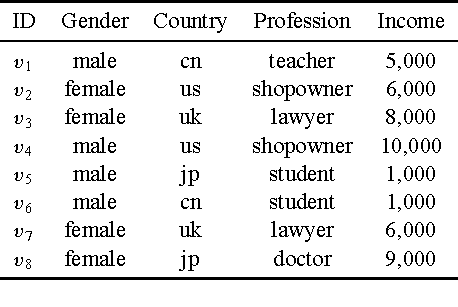
\includegraphics[width=0.27\textwidth]{fig/example/example_tables/tb_example_dataset_adjust.pdf}
		}
		\subfigure[{\scriptsize Network structure}]{
			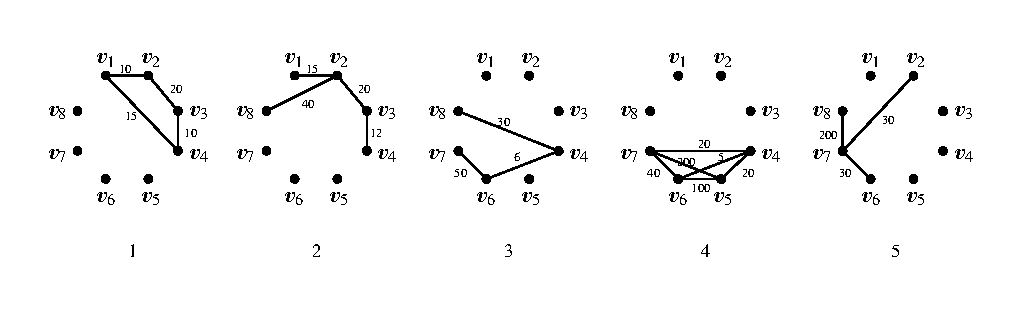
\includegraphics[width=0.63\textwidth]{fig/example/example_dataset_trade.pdf}
		}
	\end{tabular}
	\end{center}
	\vspace*{-0.4cm}
	\caption{Running example: a temporal multidimensional network with its vertex table and network structure}
	\vspace*{-0.4cm}
	\label{fig:example_dataset}
\end{figure*}

\begin{example} \label{exam:temp_multi_network}
	Fig.~\ref{fig:example_dataset} shows a sample temporal transaction network, presenting the transactions between individuals of different countries of birth and professions in each day. Table in Fig.~\ref{fig:example_dataset} (a) is the vertex table of the temporal network, showing the information of the 8 individuals. Each individual has a primary key ID and 3 dimensions (3 discrete attributes): gender, country (country of birth), profession. Income is a numeric attribute of individuals. Fig.~\ref{fig:example_dataset} (b) shows the network structure of the temporal network. There are 20 temporal edges, illustrating the transactions between individuals in 5 days. Temporal edges in each day can be organized into a snapshot. The numeric attribute on each temporal edge is the amount of each transaction. The static multidimensional information of individuals in Fig.~\ref{fig:example_dataset} (a) and the temporal information of network structure in Fig.~\ref{fig:example_dataset} (b) form a temporal multidimensional network.
\end{example}
In static graph cube \cite{zhao2011graph}, users can specify different views to obtain summarized information of the static multidimensional network and combine the information under these views through OLAP operations such as roll-up, drill-down and slice-and-dice interactively for decision support and business intelligence. For example, a company tries to use static graph cube to analyze the interaction characteristics of people with different attributes (name, gender, profession, income level, etc.) in a large-scale social network in order to support their marketing strategy making. However, edges in real-world networks usually contain timestamps. For example, in social networks, interactions between people occur at specific times, such as a particular day. In this way, static graph cube does not work when users only need information for a specific time range. Considering the previous example, the company only needs data from the last few years, because data that is too old is less informative. Or, they want to study what the characteristics of people's interactions are during particular time ranges, such as holidays or COVID-19 periods. Or, they wish to compare several different time ranges to see how people's interaction patterns change over time. Static graph cube cannot meet the above requirements. As a result, we need to propose novel approaches to make data warehouses and OLAP capable of analyzing temporal multidimensional networks.

\comment{
\begin{figure}[t!]
	\begin{center}
		\begin{tabular}[t]{c}
			\centering
			\hspace*{+0.3cm}
			\subfigure[{\scriptsize Vertex table}]{
				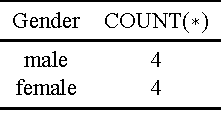
\includegraphics[width=0.36\columnwidth]{fig/example/example_tables/tb_cuboid_gender_adjust.pdf}
			}
			\hspace*{-0.6cm}
			\subfigure[{\scriptsize Network structure}]{
				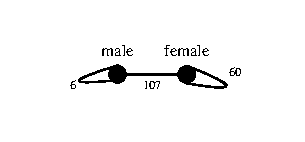
\includegraphics[width=0.58\columnwidth]{fig/example/exam_cuboid_gender_2_3.pdf}
			}
			\hspace*{-0.6cm}
		\end{tabular}
	\end{center}
	\vspace*{-0.4cm}
	\caption{The answer to ``What is the amount of transactions between individuals of different genders from day 2 to day 3?"}
	\vspace*{-0.4cm}
	\label{fig:exam_cuboid_gender}
\end{figure}
\begin{figure}[t!]
	\begin{center}
		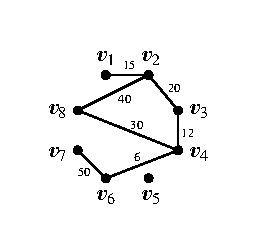
\includegraphics[width=0.45\columnwidth]{fig/example/exam_cuboid_gender_semi_state.pdf}
	\end{center}
	\vspace*{-0.7cm}
	\caption{Intermediate result of generating network structure in Fig.~\ref{fig:exam_cuboid_gender} (b)}
	\vspace*{-0.4cm}
	\label{fig:exam_inter_result_gender}
\end{figure}

}

%\begin{table}[t!]%\vspace*{-0.3cm}
%	%\scriptsize
%	\small
%	\centering
%	\caption{Vertex table of the first question in Example~\ref{exam:cuboid_query}} \vspace*{-0.2cm} \label{tab:cuboid_gender}
%	\begin{tabular}{c c}
%		\toprule
%		Gender & COUNT($\ast$) \cr %\hline %\hline
%		\midrule
%		male&4 \cr %\hline
%		female&4  \cr %\hline
%		\bottomrule
%	\end{tabular}
%	\vspace*{0.4cm}
%\end{table}

%\begin{figure*}[t!]
%	\begin{center}
%		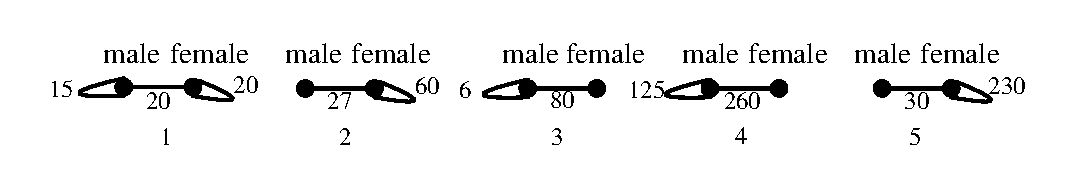
\includegraphics[width=0.95\textwidth]{fig/example/exam_aggregate_gender.pdf}
%	\end{center}
%	\vspace*{-0.4cm}
%	\caption{example aggregate gender}
%	\vspace*{-0.4cm}
%	\label{fig:aggregation_gender}
%\end{figure*}

%\begin{table}[t!]%\vspace*{-0.3cm}
%	%\scriptsize
%	\small
%	\centering
%	\caption{Vertex table of the second and the third question in Example~\ref{exam:cuboid_query}} \vspace*{-0.2cm} \label{tab:cuboid_gender_profession}
%	\begin{tabular}{c c c}
%		\toprule
%		Gender & Profession & AVERAGE($\ast$) \cr %\hline %\hline
%		\midrule
%		male & teacher& 5,000 \cr %\hline
%		male & shopowner & 10,000  \cr %\hline
%		male & student & 1,000  \cr %\hline
%		female & shopowner & 6,000  \cr %\hline
%		female & lawyer & 7,000  \cr %\hline
%		female & doctor & 9,000  \cr %\hline
%		\bottomrule
%	\end{tabular}
%	\vspace*{-0.4cm}
%\end{table}

%\begin{figure*}[t!]
%	\begin{center}
%		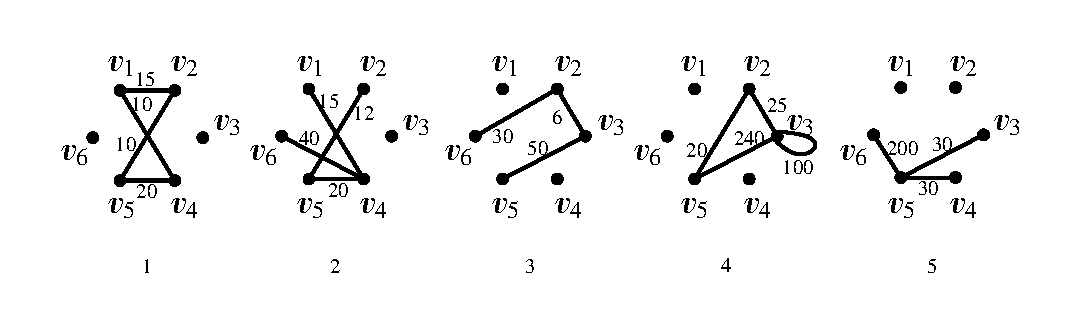
\includegraphics[width=0.95\textwidth]{fig/example/exam_aggregate_gender_pro.pdf}
%	\end{center}
%	\vspace*{-0.4cm}
%	\caption{example aggregate gender profession}
%	\vspace*{-0.4cm}
%	\label{fig:aggregation_gender_profession}
%\end{figure*}
%


%\begin{figure}[t!]
%	\begin{center}
%		\begin{tabular}[t]{c}\hspace*{-0.3cm}
%			\subfigure[{\scriptsize Structure of the answer of the first question in Example~\ref{exam:cuboid_query}}]{
%				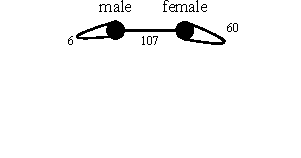
\includegraphics[width=0.45\columnwidth]{fig/example/exam_cuboid_gender_2_3_adjust.pdf}
%			}
%			\subfigure[{\scriptsize The intermediate result of generating (a)}]{
%				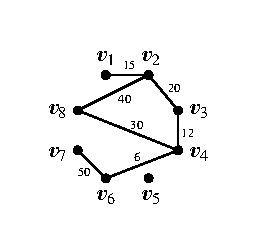
\includegraphics[width=0.45\columnwidth]{fig/example/exam_cuboid_gender_semi_state.pdf}
%			}
%		\end{tabular}
%	\end{center}
%	\vspace*{-0.4cm}
%	\caption{}
%	\vspace*{-0.4cm}
%	\label{fig:exam_cuboid_gender}
%\end{figure}

\comment{
\begin{figure}[t!]
	\begin{center}
		\begin{tabular}[t]{c}\hspace*{-0.2cm}
			\subfigure[{\scriptsize Vertex table}]{
				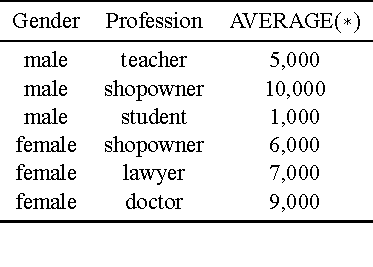
\includegraphics[width=0.4\columnwidth]{fig/example/example_tables/tb_cuboid_gender_pro_adjust.pdf}
			}
			\subfigure[{\scriptsize Network structure from day 2 to day 3}]{
				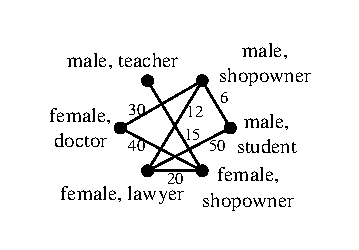
\includegraphics[width=0.5\columnwidth]{fig/example/exam_cuboid_gender_pro_2_3.pdf}
			}
			%\vspace*{-0.3cm}\\\hspace*{-0.3cm}
			\\
			\subfigure[{\scriptsize Network structure from day 4 to day 5}]{
				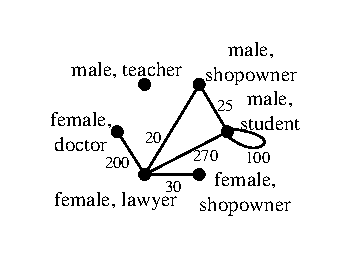
\includegraphics[width=0.5\columnwidth]{fig/example/exam_cuboid_gender_pro_4_5.pdf}
			}
		\end{tabular}
	\end{center}
	\vspace*{-0.4cm}
	\caption{The answers to ``What is the amount of transactions between individuals of different genders and professions from day 2 to day 3 and from day 4 to day 5?"}
	\vspace*{-0.4cm}
	\label{fig:exam_cuboid_gender_profession}
\end{figure}
\begin{example} \label{exam:cuboid_query}
	Fig.~\ref{fig:exam_cuboid_gender} shows a static aggregate network obtained by summarizing the temporal multidimensional network in Fig.~\ref{fig:example_dataset} on dimension ``Gender'' and time range $ [2,3] $. Fig.~\ref{fig:exam_cuboid_gender} can be regarded as the answer of question ``What is the amount of transactions between individuals of different genders from day 2 to day 3?" Note that the vertex table in Fig.~\ref{fig:exam_cuboid_gender} (a) is directly aggregated from the vertex table in Fig.~\ref{fig:example_dataset} (a) on ``Gender" with COUNT($\ast$) as aggregation function on vertices. All vertices in Fig.~\ref{fig:example_dataset} (a) are included in the aggregation process even those vertices which have no adjacent edge in day 2 and day 3, like $ v_5 $. The reason is that vertices are time independent and vertices having no adjacent edge in specified time ranges are still available in those time ranges. Therefore, from day 2 to day 3, the COUNT($\ast$) value of male should be 4. Fig.~\ref{fig:exam_inter_result_gender} shows the intermediate result of the question, which is obtained by merging all snapshots in day 2 and day 3. All edges of snapshots in day 2 and day 3 are collected to the single snapshot in Fig.~\ref{fig:exam_inter_result_gender}, and if there are two edges in snapshots of day 2 and day 3 respectively share the same vertices, then their numeric attributes will be added together since SUM($\ast$) is the aggregation function upon edges here. Fig.~\ref{fig:exam_cuboid_gender} (b) can be directly aggregated from Fig.~\ref{fig:exam_inter_result_gender} on the basis of aggregated vertices in Fig.~\ref{fig:exam_cuboid_gender} (a), i.e., each edge in Fig.~\ref{fig:exam_cuboid_gender} (b) is the aggregated edge of edges in Fig.~\ref{fig:exam_inter_result_gender}, whose two vertices are aggregated to the two vertices of the corresponding aggregated edge. The numeric attributes of the aggregated edges in Fig.~\ref{fig:exam_cuboid_gender} (b) are still the sum of attributes of their corresponding sets of edges in Fig.~\ref{fig:exam_inter_result_gender}.
	
	Finally, we can reply the question above. For example, from day 2 to day 3, the amount of transactions between males is 6, while the amount of transactions between male and female is 107, etc. Fig.~\ref{fig:exam_cuboid_gender_profession} shows the answers of two similar questions ``What is the amount of transactions between individuals of different genders and professions from day 2 to day 3 and from day 4 to day 5?" The only difference between these two questions is the time range specified. Both static aggregate networks in Fig.~\ref{fig:exam_cuboid_gender_profession} share the same vertex table in Fig.~\ref{fig:exam_cuboid_gender_profession} (a) and in these two questions the aggregation functions upon vertices are AVERAGE($\ast$).
\end{example}


There are three new OLAP queries in Example~\ref{exam:cuboid_query} compared to queries in static graph cube, for example, the first OLAP query in Example~\ref{exam:cuboid_query} is ``What is the amount of transactions between individuals of different genders from day 2 to day 3", which requests a rough summarized result of the temporal multidimensional network in Fig.~\ref{fig:example_dataset} on ``Gender". Unlike the query in static graph cube, this new query includes a specific time range $ [2,3] $. Conducting the new query includes the same aggregation on vertex table as in static graph cube, but when aggregating the network structure, the basic idea is to first merge snapshots in the time range to build an intermediate result, as shown in Fig.~\ref{fig:exam_inter_result_gender}, then perform the same aggregation on Fig.~\ref{fig:exam_inter_result_gender} as in static graph cube. If the new query specifies the whole time range of the temporal multidimensional network, then it is equivalent to a query in static graph cube. Therefore, static graph cube is a special case of the new data warehouse model proposed in this paper. Conducting the second OLAP query ``What is the amount of transactions between individuals of different genders and professions from day 2 to day 3" can be regarded as performing a drill-down operation on the basis of the first query, since the second query requests more fine-grained information in the same time range than the first query. The third query ``What is the amount of transactions between individuals of different genders and professions from day 4 to day 5" specifies the same dimensions as the second query, but specifies a different time range $ [4,5] $. This allows users to analyze the pattern characteristics in different time ranges, for example, there is no transaction between male students from day 2 to day 3, but there are transactions totaling 100 between them from day 4 to day 5. Note that the aggregation functions upon vertices and edges can be combined arbitrarily as needed. For example, we can specify AVERAGE($\ast$) as the aggregation function upon both vertices and edges in Example~\ref{exam:cuboid_query}, so that we can analyze the transaction network from another perspective.

In \cite{zhao2011graph}, Zhao et al.\ proposed a new OLAP query for static multidimensional networks, called \kw{crossboid}, to analyze the crossed interaction pattern of two different views. It is easy to see that \kw{Crossboid} can also be extended to temporal multidimensional networks as illustrated in Example~\ref{exam:crossboid_query}.

\begin{table}[t!]%\vspace*{-0.3cm}
	%\scriptsize
	\small
	\centering
	\caption{Vertex table obtained by group-by on ``Profession" in Fig.~\ref{fig:example_dataset} (a)} \vspace*{-0.2cm} \label{tab:groupby_profession}
	\begin{tabular}{c c}
		\toprule
		Profession & COUNT($\ast$) \cr %\hline %\hline
		\midrule
		teacher& 1 \cr %\hline
		shopowner & 2  \cr %\hline
		student & 2  \cr %\hline
		lawyer & 2  \cr %\hline
		doctor & 1  \cr %\hline
		\bottomrule
	\end{tabular}
	\vspace*{-0.4cm}
\end{table}

\begin{figure}[t!]
	\begin{center}
		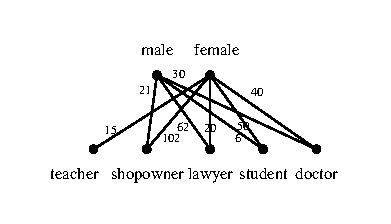
\includegraphics[width=0.85\columnwidth]{fig/example/exam_crossboid_gender_pro_2_3.pdf}
	\end{center}
	\vspace*{-0.7cm}
	\caption{Structure of the answer to the question in Example~\ref{exam:crossboid_query}}
	\vspace*{-0.4cm}
	\label{fig:exam_crossboid_gender_profession}
\end{figure}

\begin{example} \label{exam:crossboid_query}
	Fig.~\ref{fig:exam_crossboid_gender_profession} shows the structure of the answer to ``What is the amount of transactions between individuals grouped by gender and individuals grouped by profession from day 2 to day 3?" The answer can also be regarded as a static aggregate network which has two vertex tables from group-by on ``Gender" and ``Profession" shown in Fig.~\ref{fig:exam_cuboid_gender} (a) and Table~\ref{tab:groupby_profession} respectively. Fig.~\ref{fig:exam_crossboid_gender_profession} shows the crossed transactions between two different views ``Gender" and ``Profession" from day 2 to day 3, e.g., for all transactions between males and individuals of different professions, all 4 males have the biggest amount of transactions with the 2 lawyers and the smallest amount of transactions with the 2 students from day 2 to day 3. Other crossed transactions can also be easily found in Fig.~\ref{fig:exam_crossboid_gender_profession}.
\end{example}
}

In this paper, we propose a new data warehouse model, called \kw{Temporal} \kw{Graph} \kw{Cube}; and we extend the definition of OLAP queries by specifying a time range so that they can be applied to \kw{Temporal} \kw{Graph} \kw{Cube}. Users can explore summarized information on different views of temporal multidimensional networks in any time range using \kw{Temporal} \kw{Graph} \kw{Cube}. The challenge of our problem is: how to efficiently merge snapshots in a specific time range for each online OLAP query. A basic approach is to merge snapshots in the time range one by one. Such a basic method, however, is clearly inefficient when the time ranges are very large or a large number of OLAP queries come. The above problem can be seen as range query on snapshot arrays. Unfortunately, among the existing works for summarizing temporal networks \cite{liu2018graph}, there is no work which focuses on summarizing snapshots within a certain time range online. In this paper, we investigate the problem of how to speed up merging snapshots in certain time ranges. Our solution is to build an index on snapshot arrays to reduce the query processing time. Specifically, we propose a segment-tree based index to support the range query on snapshot arrays. Since new edges are constantly inserted into the temporal multidimensional network, we also propose an index updating technique to handle such an edge-insertion case. In addition, similar to the static graph cube, the implementation of the \kw{Temporal} \kw{Graph} \kw{Cube} also requires determining the materialization strategy of views in order to achieve a balance between time and space. To this end, we adopt a strategy called \kw{MinLevel} proposed in \cite{zhao2011graph} to handle the materialization problem in \kw{Temporal} \kw{Graph} \kw{Cube}, as it fits our model best.

To summarize, the main contributions of this work are as follows:
\begin{enumerate}
	\item We propose a new data warehouse model \kw{Temporal} \kw{Graph} \kw{Cube}, which supports decision making on the basis of temporal multidimensional networks. The key difference compared to static graph cube is that \kw{Temporal} \kw{Graph} \kw{Cube} supports querying summarized information for any time range of temporal multidimensional networks so that it supports more diverse analysis.
	
	\item We extend the classic segment tree that tailored for traditional range query problems to our range query problems on snapshot arrays to reduce the OLAP query processing time. We also develop \revision{an} index maintainable technique to handle the case when new edges are added to the temporal networks. %Similar requirement has not been seen on common range query problems.
	
	\item  We propose a new metric, called \kw{similarity\enspace of\enspace snapshots}, to measure the overall similarity of snapshots in a snapshot array, or, the degree to which the edges are shared by different snapshots. We show that this metric has a strong correlation with the effectiveness of the indexes and it can guide us to decide whether an index should be built.

	
%	\item We point out that the existing methods used to implement traditional data cube and static graph cube: greedy algorithm \cite{harinarayan1996implementing} and its variants \cite{morfonios2007rolap}, are no longer applicable in \kw{Temporal \enspace Graph \enspace Cube} scenario. The main reason is that OLAP queries contain arbitrary time ranges. A more reasonable method is \kw{MinLevel}, which is easy to be implemented and does not take into account the time ranges in OLAP queries.
	
	\item We conduct extensive experiments on two large-scale real-world datasets. The results demonstrate the effectiveness and efficiency of the \kw{Temporal \enspace Graph \enspace Cube}. The results also confirm the correlation between the efficiency (time and space) of the index and \kw{similarity\enspace of\enspace snapshots}. %We also examined the update performance of our index. Among them, we find that the segment tree index is with the best time and space balance and scalability among the three indexes.
\end{enumerate}

\comment{
%\vspace*{-0.2cm}
\stitle{Organizations.} Section~\ref{sec:temp_graph_cube} introduces the details about \kw{Temporal \enspace Graph \enspace Cube}. We extend all three indexes to snapshot array in Section~\ref{sec:indexes}. In Section~\ref{sec:effec_of_indexes} we discuss a metric, \kw{similarity\enspace of\enspace snapshots}, which affects the efficiency of indexes and how it affects. Section~\ref{sec:partial_materialization} introduces the implementation of \kw{Temporal \enspace Graph \enspace Cube}. We conduct experiments in Section~\ref{sec:experiment} and review the related works in Section~\ref{sec:related_work}. We conclude our work in Section~\ref{sec:conclusion}.
}

\section{Temporal Graph Cube} \label{sec:temp_graph_cube}
%\subsection{Notations and Basic Concepts} \label{subsec:notation}
%\vspace*{-0.1cm}
%\subsection{Definitions}\label{subsec:definitions}
\begin{definition}[Temporal Multidimensional Network]
	\label{def:temp_multi_network}
	Let $\Gr=(\Vr, \Er, A, W)$ be an undirected temporal multidimensional network where $\Vr$ and $\Er$ are the set of nodes and edges respectively. Edges in $\Er$ are in the form of $(u, v, t, a)$. \revision{$ u $ and $ v $ are nodes in $\Vr$. $ t $ and $ a $ are timestamp and numeric attribute respectively attached to edges}. $A=\{A_1, A_2, ... , A_n\}$ represents the dimensions of the network or $n$ discrete attributes of nodes in $ \Vr $, i.e., $A(u)=\{A_1(u), A_2(u), ... , A_n(u)\}$ where $A_i(u)$ is the actual value of $u$ on the $i$-th attribute. $ W(u) $ is the numeric value of $u$.
\end{definition}

For convenience, we abbreviate temporal multidimensional network and static multidimensional network to temp-multi-network and static-multi-network respectively. Since we only consider undirected edges in this paper, if not specified, we assume without loss of generality $u \leq v$ for $(u, v, t, a)$ in all following definitions. As shown in Fig.~\ref{fig:example_dataset}, $ A=\{Gender,Country,Profession\} $ and $ W=Income $. We do not consider ID to be an attribute of individuals because ID is only the identification of individuals. $ \Vr $ is the set of IDs of individuals in Fig.~\ref{fig:example_dataset} (a) and $ \Er $ is the set of temporal edges in Fig.~\ref{fig:example_dataset} (b). A temp-multi-network can also be represented by a sequence of snapshots.

\begin{definition}[Snapshot]
	\label{def:snapshot}
	Let $\Tr=\{t|(u, v, t, a)\in \Er\}$ be the set of timestamps. For each $t_i\in \Tr$, we can obtain a snapshot $S_i=\{(u,v,a)|(u,v,t_i,a)\in \Er\}$.
\end{definition}

For example, in Fig.~\ref{fig:example_dataset} (b), we can extract 5 snapshots; and the snapshot at timestamp 1 is $ S_1=\{(v_1,v_2,10),(v_2,v_3,20),(v_3,v_4,10),(v_1,v_4,15)\} $. With the definition of snapshot, we can define temp-multi-network in Definition~\ref{def:temp_multi_network} as $\Gr=(\Vr,\Sr,A,W)$ where $\Sr=\{S_1,S_2,...,S_{|\Tr|}\}$ and $ S_i $ is the snapshot at $t_i$.

\stitle{Biased Timestamp.} To store snapshots in a snapshot array and access snapshots directly by corresponding timestamps, we replace the original timestamps of snapshots with \emph{biased timestamps}. For each temp-multi-network, suppose $ t_1 $ is the smallest timestamp, $ t_{|\Tr|} $ is the biggest timestamp and $ t_{base}=t_1-1 $, biased timestamp of snapshot $ S_i $ is computed by $ t_i-t_{base} $. Through biased timestamp we can map timestamps in $ [t_1,t_{|\Tr|}] $ to $ [1,t_{end}] $, where $ t_{end}=t_{|\Tr|}-t_{base} $. The above strategy is useful when timestamps in temp-multi-network are dense. If timestamps are sparse, i.e., $ |\Tr| \ll t_{|\Tr|}-t_1 $, there will be many empty snapshots in snapshot array. We can sacrifice a little in efficiency, hashing all the timestamps into a denser space and relocating time range $ [l,r] $ of each query (we will discuss queries in Section~\ref{sec:queries}) to the actual time range. However, in large scale real-world temp-multi-networks, temporal relations can be built at almost all time, so the timestamps are unlikely to be sparse, which is confirmed in our datasets. All algorithms in this paper are designed based on the definition of temp-multi-network $\Gr=(\Vr,\Sr,A,W)$, where $ \Sr $ is a snapshot array with biased timestamps of snapshots start from 1.

\comment{
Aggregation, or traditional group-by, is a key operation in data warehouses and OLAP for traditional RDB data and static-multi-network. In traditional RDB data, for an aggregation in form of $(A_1',A_2',...,A_n')$ where some (or all) dimension $A_i'$ could be $\ast$ (ALL), the result is another table in which tuples in source table having the same value in all specified dimensions (NOT $\ast$) are grouped in the same tuple. In the above process, numeric attributes of tuples in source table can be summed by aggregation functions, e.g., COUNT($\ast$), AVERAGE($\ast$), MAX($\ast$) and MIN($\ast$). In static-multi-network, aggregations are not only conducting group-by on the vertex table but constructing static aggregate networks and computing the aggregation result of attributes of edges using specified aggregation function. The results of aggregations on static-multi-network, static aggregate networks, are exactly the answers of OLAP queries on static-multi-network \cite{zhao2011graph}. However, situations are different in temp-multi-networks. Below, we first define temporal aggregate network (the results of aggregations on temp-multi-network), and show the difference between static aggregate network and temporal aggregate network. Then, we describe the benefit of temporal aggregate network in conducting OLAP queries on temp-multi-network.
}

\begin{definition}[Temporal Aggregate Network]
	\label{def:temp_aggregate_network}
	Given a temporal multidimensional network $\Gr=(\Vr,\Sr,A,W)$ and an aggregation $A'=(A'_1,A'_2,...,A'_n)$ where $A'_i$ equals $A_i$ or $\ast$, the obtained temporal aggregate network is another temporal multidimensional network $\Gr'=(\Vr',\Sr',B,W_{\Gr'})$ where $\Vr' \subseteq \Vr$, $B=\{A'_i|A'_i \neq \ast\}$ and
	\begin{enumerate}
		\item \revision{Let $ [v] $ be an equivalence class of $ v $, where $ v \in \Vr $ and $[v]=\{u|B(u)=B(v),u \in \Vr\}$. For each $ v\in \Vr $, $ \exists v' \in \Vr'$ satisfying $v' \in [v]$ and $\nexists u' \in \Vr', u' \neq v'$ satisfying $u' \in [v]$.} $W_{\Gr'}(v')$ is the aggregation result of $W(v)$ for $v \in [v']$ obtained by aggregation function upon vertices specified by user.
%		\item For any $S'_i$ in $\Sr'$ and each $(u',v',a')$ in $S'_i$, there exists a nonempty maximum edge set $E=\{(u,v,a)|(u,v,a) \in S_i, u \in [u'] \wedge v \in [v']\; or\; u \in [v'] \wedge v \in [u']\}$, $a'$ is the aggregation result of numeric attributes ($a$) of edges in $E$ obtained by aggregation function specified by user.
		\item $\forall u',v' \in \Vr'$ where $u' \leq v'$ and any $\Sr[i], i \in [1,t_{end}]$, if there exists a nonempty maximum edge set $E=\{(u,v,a)|(u,v,a) \in \Sr[i],(u \in [u'] \wedge v \in [v']) \vee (u \in [v'] \wedge v \in [u']) \}$, then $ \exists (u',v',a') \in \Sr'[i] $, where $a'$ is the aggregation result of numeric attributes of edges in $E$ obtained by aggregation function upon edges specified by user.
	\end{enumerate}
\end{definition}
In short, conducting aggregations on temp-multi-network contains two stages: aggregating, or group-by on the vertex table as 1) in Definition~\ref{def:temp_aggregate_network} and aggregating each snapshots in the temp-multi-network as 2) in Definition~\ref{def:temp_aggregate_network}.

\begin{figure}[t!]
	\begin{center}
		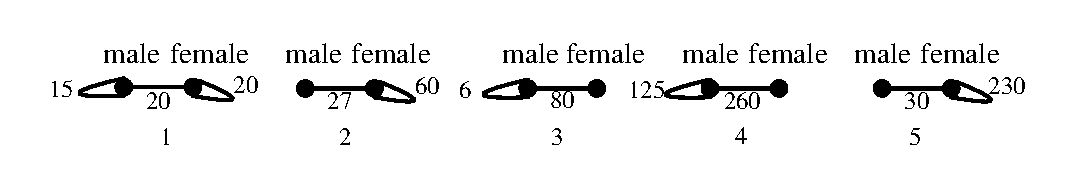
\includegraphics[width=0.95\columnwidth]{fig/example/exam_aggregate_gender.pdf}
	\end{center}
	\vspace*{-0.9cm}
	\caption{Snapshots of the first temporal aggregate network in Example~\ref{exam:temporal_aggregate_network}}
	\vspace*{-0.4cm}
	\label{fig:aggregation_gender}
\end{figure}

\begin{figure}[t!]
	\begin{center}
		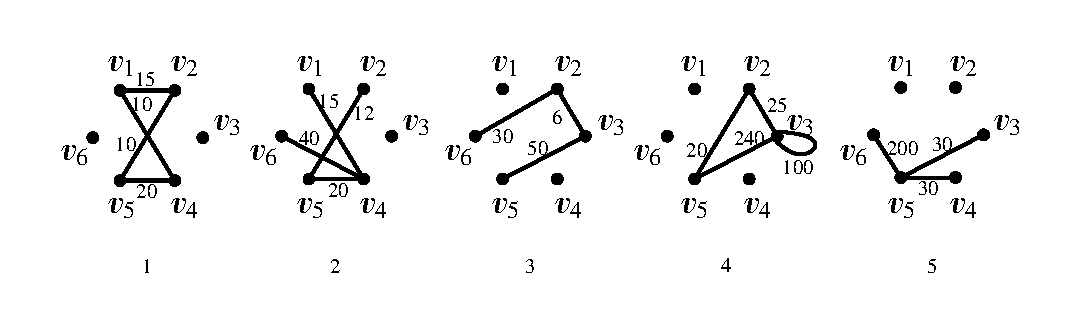
\includegraphics[width=0.95\columnwidth]{fig/example/exam_aggregate_gender_pro.pdf}
	\end{center}
	\vspace*{-0.9cm}
	\caption{Snapshots of the second temporal aggregate network in Example~\ref{exam:temporal_aggregate_network}. $ v_1= $ ``male, teacher", $ v_2= $ ``male, shopowner", $ v_3= $ ``male, student", $ v_4= $ ``female, shopowner", $ v_5= $ ``female, lawyer", $ v_6= $ ``female, doctor"}
	\vspace*{-0.4cm}
	\label{fig:aggregation_gender_profession}
\end{figure}

\begin{example} \label{exam:temporal_aggregate_network}
	Fig.~\ref{fig:aggregation_gender} shows the snapshots of a temporal aggregate network, which is obtained by aggregating temp-multi-network in Fig.~\ref{fig:example_dataset} on dimension ``Gender". The obtained temporal aggregate network is also a temp-multi-network. There are 5 snapshots in Fig.~\ref{fig:aggregation_gender}, each of them is corresponding to the snapshot with the same timestamp in Fig.~\ref{fig:example_dataset} (b). For each snapshot in Fig.~\ref{fig:aggregation_gender}, each edge $ e' $ is the aggregated edge of a set of edges $ E $ in the corresponding snapshot. Each edge in $ E $ have two vertices aggregated to the two vertices of $ e' $, as 2) in Definition~\ref{def:temp_aggregate_network}. In this example, the attribute in $ e' $ is the amount of the attributes of edges in $ E $, i.e., the total transactions between individuals of two genders in each day. We can also choose other aggregation functions for edges like COUNT($\ast$), MAX($\ast$), and so on. Similarly, Fig.~\ref{fig:aggregation_gender_profession} shows another temporal aggregate network by aggregating temp-multi-network in Fig.~\ref{fig:example_dataset} on dimension ``Gender" and ``Profession".
\end{example}

%As in Example~\ref{exam:temporal_aggregate_network}, Fig.~\ref{fig:aggregation_gender} and Fig.~\ref{fig:aggregation_gender_profession} are temporal aggregate networks $ \Gr'_1 $ and $ \Gr'_2 $ aggregated from Fig.~\ref{fig:example_dataset} on $ (Gender,\ast,\ast) $ and $ (Gender,\ast,Profession) $ respectively. For $ \Gr'_1=(\Vr'_1,\Sr'_1,B_1,W'_1) $, $ \Vr'_1 $ is the set of nodes, which are represented by tuples in "Gender" column of Table~\ref{tab:aggregation_gender}. $ \Sr'_1 $ is the snapshot array starting from subscript 1 and storing the 5 snapshots in Fig.~\ref{fig:aggregation_gender}. $ B_1=\{Gender\} $. $ W'_1 $ is the mapping from $ \Vr'_1 $ to COUNT($\ast$) value of nodes in $ \Vr'_1 $ as shown in "COUNT($\ast$)" column in Table~\ref{tab:aggregation_gender}. The aggregation function upon edges is SUM($\ast$). For $ \Gr'_2 $, [mention it in introduction].

\comment{
From Definition~\ref{def:temp_aggregate_network} and Example~\ref{exam:temporal_aggregate_network}, we can find that aggregation on static-multi-network is a special case of aggregation on temp-multi-network, if there is only one snapshot in temp-multi-network. For most cases, compared to aggregation on static-multi-network, aggregation on temp-multi-network contains aggregating each snapshot of the temp-multi-network to condensed snapshot independently.
}

Obviously, the temporal aggregate network is not the direct answer of OLAP query on temp-multi-network, because temporal aggregate network contains aggregated snapshot at each timestamp, but OLAP query on temp-multi-network requires a summarized snapshot of a specified time range. However, temporal aggregate network can provide a cheaper way to conduct queries compared to conducting queries directly on the original temp-multi-network. We will explain in detail in Section~\ref{sec:queries}. %For example, the snapshot in Fig.~\ref{fig:exam_cuboid_gender} (b) can be obtained by merging snapshots in day 2 and day 3 in Fig.~\ref{fig:aggregation_gender}, without generating the intermediate result in Fig.~\ref{fig:exam_inter_result_gender}. We will explain in detail in Section~\ref{subsec:queries}.

\begin{algorithm}[t]
	\scriptsize
	\caption{$\kw{Temporal Aggregate Network Construction}$}
	\label{alg:view_construct_baseline}
	\KwIn{A temp-multi-network $\Gr=(\Vr,\Sr,A,W)$; Aggregation $A'$; Aggregation function $f_v$ and $f_e$ upon vertices and edges respectively}
	\KwOut{Temporal aggregate network $\Gr'=(\Vr',\Sr',B,W_{\Gr'})$, $B=\{A'_i|A'_i \neq \ast\}$}
	$ \Vr' \gets \{\} $, let $ h $ be hash structure: $ \{B(u)|u \in \Vr\} \rightarrow \Vr' $;
	
	\ForEach{$u \in \Vr$}{
		\If{$h(B(u))=NULL$}{
			$ \Vr' \gets \Vr' \cup \{u\} $;
			$ W_{\Gr'}(u) \gets W(u) $;
			$ h(B(u)) \leftarrow u $;
		}
		\Else{
			$ u' \gets h(B(u)) $;
			$ W_{\Gr'}(u') \gets f_v(W_{\Gr'}(u'),W(u)) $;
		}
	}
	$ \Sr' \gets $ a snapshot array with $ t_{end}+1 $ empty snapshots;

	\ForEach{$ i \in [1,t_{end}] $}{
		$ EP \gets \{\} $;
		
		\ForEach{$ (u,v,a) \in \Sr[i] $}{
			$u' \gets h(B(u))$;
			$v' \gets h(B(v))$;
			
			\lIf{$ u'>v' $}{
				$ u',v' \gets v',u' $
			}
			
			\If{$(u',v') \notin EP$}{
				$ EP \gets EP \cup \{(u',v')\}$;
				$ \Sr'[i] \gets \Sr'[i] \cup \{(u',v',a)\} $;
			}
			\Else{
				Let $ (u',v',a') $ be edge in $\Sr'[i]$ which has $ u',v' $ as vertices\;
				$ \Sr'[i] \gets \Sr'[i]-\{(u',v',a')\} $\;
				$ \Sr'[i] \gets \Sr'[i] \cup \{(u',v',f_e(a',a))\} $;
			}
		}
	}
	\Return $ \Gr'=(\Vr',\Sr',B,W_{\Gr'}) $;
\end{algorithm}

We devise a basic algorithm, as outlined in Algorithm~\ref{alg:view_construct_baseline},  to construct the temporal aggregate network with aggregation $ A' $ from the original network $ \Gr $. Note that there are two things to be concerned about aggregation functions:
\begin{itemize}[leftmargin=*]
	\item We assume $ f_v $ and $ f_e $ are not AVERAGE($\ast$), since the result of AVERAGE($\ast$) can be easily computed by SUM($\ast$)/COUNT($\ast$).
	
	\item If $ f_v =$ COUNT($\ast$), we assign $1$ to all $ W(u),u \in \Vr $, because $ 1 $ is the correct attribute value of each vertex when counting is needed. The same assignment should be done to numeric attributes of all edges if $ f_e= $ COUNT($\ast$).
\end{itemize}
Algorithm~\ref{alg:view_construct_baseline} first conducts the specified aggregation on all vertices of the original network. In line~1, we first create a hash structure, $h$, to maintain a mapping from all possible $ B(u),u \in \Vr $ to vertices of the temporal aggregate network. In lines~2-6, we group all vertices in $ \Vr $ with the specified aggregation $ A' $ and compute the aggregation result of numeric attributes of vertices with the specified aggregation function $ f_v $. Each snapshot $ \Sr[i] $ of $ \Gr $ is aggregated into a smaller representation, i.e., the corresponding snapshot $ \Sr'[i] $ at the same timestamp in $ \Gr' $ (lines~8-18). For each edge $ (u,v,a) $, we first map the two vertices $ u,v $ to $ u',v' $ using $ h $ (line~11-12). If there exists an aggregated edge $ (u',v',a') $ in $ \Sr'[i] $, we update $ a' $ with $ a $ using $ f_e $ (lines~16-18), otherwise we insert $ (u',v',a) $ into $ \Sr'[i] $ directly (line~14).

It is easy to derive that the time complexity of Algorithm~\ref{alg:view_construct_baseline} is $ O(|\Vr|+\sum_{i=1}^{t_{end}}{|\Sr[i]|}) $. The space used to maintain $ h,W_{\Gr'} $ is $ O(\Vr') $ and we need $ O(|\Vr'|+\sum_{i=1}^{t_{end}}{|\Sr'[i]|}) $ space to maintain $ \Gr' $. Moreover, we can easily derive that $ |\Vr'| \leq |\Vr| $ and $ |\Sr'[i]| \leq |\Sr[i]| $. As a result, the space complexity of Algorithm~\ref{alg:view_construct_baseline} is $ O(|\Vr|+\sum_{i=1}^{t_{end}}{|\Sr[i]|}) $.

%The time complexity of Algorithm~\ref{alg:view_construct_baseline} is $ O(|\Vr|+\sum_{i=1}^{t_{end}}{|\Sr[i]|}) $, which contains time used for traversing $ \Vr $ and $ \Sr $. The space used to maintain $ h,W_{\Gr'} $ is $ O(\Vr') $ and we need $ O(|\Vr'|+\sum_{i=1}^{t_{end}}{|\Sr'[i]|}) $ space to maintain $ \Gr' $. From Algorithm~\ref{alg:view_construct_baseline} we can easily find $ |\Vr'| \leq |\Vr| $ and $ |\Sr'[i]| \leq |\Sr[i]| $, so the space complexity of Algorithm~\ref{alg:view_construct_baseline} is also $ O(|\Vr|+\sum_{i=1}^{t_{end}}{|\Sr[i]|}) $.

\comment{
Similar to the static aggregate network in static graph cube, temporal aggregate networks can also be constructed from other existing temporal aggregate networks. For example, the temporal aggregate network with dimensions $ \{B_1,B_2\} $ can be constructed from the temporal aggregate network with dimensions $ \{B_1,B_2,B_3\} $, $ \{B_1,B_2,B_4\} $. The proof can be easily obtained by extending the proof from \cite{zhao2011graph}.
}

\begin{definition}[Temporal Graph Cube]
	\label{def:temp_graph_cube}
	Given a temporal multidimensional network $\Gr=(\Vr,\Sr,A,W)$, the temporal graph cube is obtained by decomposing $ A $ into all possible aggregations. Each aggregation $ A' $ is a node in the temporal graph cube and it corresponds to a temporal aggregate network $ \Gr' $ as defined in Definition~\ref{def:temp_aggregate_network}.
\end{definition}

In \cite{zhao2011graph}, Zhao et al.\ used equivalently the terms \textit{cuboid}, \textit{view} and \textit{aggregation}. In this paper, however, we only use \textit{view} and \textit{aggregation} equivalently, while \textit{temporal cuboid} is used to refer to temporal cuboid query. In following sections, computing a view $ A' $ means materializing the corresponding temporal aggregate network $ \Gr' $ in memory. If $ A' $ is precomputed, then for simplicity, $ A' $ also refers to the corresponding temporal aggregate network $ \Gr' $.

For a view $ A' $ in the temporal graph cube, $ dim(A') $ denotes the set of non-$\ast$ dimensions of $ A' $, i.e., $ dim(A')=B $ where $ B $ is the discrete attributes of vertices in $ \Gr' $, the corresponding temporal aggregate network of $ A' $. For two views $ A' $ and $ A'' $, $ A' $ is an \textit{ancestor} of $ A'' $ and $ A'' $ is a \textit{descendant} of $ A' $ if $ dim(A') \subset dim(A'') $, denoted as $ A' \preceq A'' $. Especially, the base view $ A_{base} $ is a view where $ dim(A_{base})=A $, $ A $ is the dimensions of the original temp-multi-network. It is easy to see that $ A_{base} $ is a descendant of all other views. Another special view is $ A_{apex}=(\ast,\ast,...,\ast) $; and it is an ancestor of all other views in the temporal graph cube. %It is easy to check that the

%\comment{
\begin{figure}[t]
	\begin{center}
		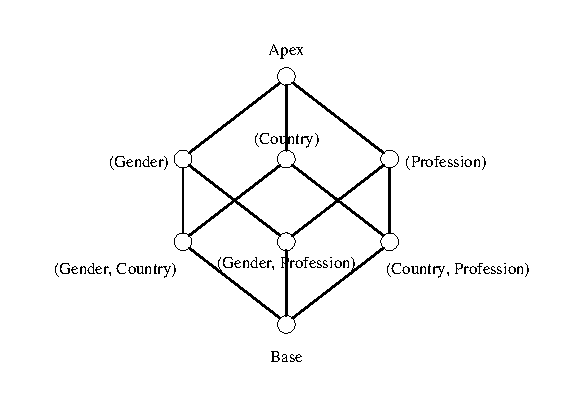
\includegraphics[width=0.75\columnwidth]{fig/example/cube_lattice.pdf}
	\end{center}
	\vspace*{-1cm}
	\caption{A sample cube lattice}
	\vspace*{-0.6cm}
	\label{fig:cube_lattice}
\end{figure}
\begin{example} \label{exam:cube_lattice}
	Fig.~\ref{fig:cube_lattice} shows the temporal graph cube lattice built on the temp-multi-network in Fig.~\ref{fig:example_dataset}, each node on the lattice represents a view. For each edge in the lattice, the upper view is an ancestor of the lower view.
\end{example}
%}

Temporal graph cube has the same form with static graph cube. The only difference is that each node in temporal graph cube is corresponding to a temporal aggregate network, not a static aggregate network. For each temporal aggregate network corresponding to a view, it contains more coarse-grained information than that of temporal aggregate network corresponding to a descendent view at each timestamp. In temporal graph cube, users can obtain summarized information in different resolution of the original temp-multi-network in a certain period by traversing the temporal graph cube lattice with specified time range. Users can also stay at some nodes in the lattice and query the summarized information in different time ranges. In these ways, summarized information of temp-multi-network in different resolutions and time ranges can be analyzed for decision support and business intelligence purposes.

%\subsection{OLAP Queries}\label{subsec:queries}
\section{Temporal OLAP Queries}  \label{sec:queries}
Cuboid and crossboid are two important OLAP queries on static-multi-networks, or in static graph cubes \cite{zhao2011graph}. In this section, we propose a generalized definition of OLAP queries in temporal graph cube, by extending cuboid and crossboid to temporal cuboid and temporal crossboid respectively. %From the previous sections, we can find that the main difference of queries in static graph cube and temporal graph cube is the designation of time range.

%\stitle{Temporal cuboid.}
\subsection{Temporal Cuboid Query} \label{subsec:cuboid}
The inputs of temporal cuboid query $ Q=(A',[l,r]) $ in temporal graph cube contain a specified view $A'=(A'_1,A'_2,...,A'_n)$ and a time range $[l,r]$. The output is a static aggregate network obtained by the query. %As illustrated in Example~\ref{exam:cuboid_query}, the first question can be represented by $ Q=((Gender),[2,3]) $, and the static aggregate network as the answer is shown in Fig.~\ref{fig:exam_cuboid_gender}.

\begin{algorithm}[t]
	\scriptsize
	\caption{$\kw{Temporal Cuboid Query}$}
	\label{alg:temp_cuboid_baseline}
	\KwIn{A temp-multi-network $\Gr=(\Vr,\Sr,A,W)$; Aggregation $A'$; Time range $[l,r]$; Aggregation function $f_v$ and $f_e$ upon vertices and edges respectively}
	\KwOut{A static aggregate network $G=(V,E,B,W_{G})$, $B=\{A'_i|A'_i \neq \ast\}$}
	$V \leftarrow \{\}$, let $h$ be hash structure: $\{B(u)|u \in \Vr\} \rightarrow V$;
	
	\ForEach{$u \in \Vr$}{
		\If{$h(B(u))=NULL$}{
			$ V \leftarrow V \cup \{u\} $;
			$ W_{G}(u) \gets W(u) $;
			$ h(B(u)) \leftarrow u $;
		}
		\Else{
			$ u'\gets h(B(u)) $;
			$ W_{G}(u') \gets f_v(W_{G}(u'),W(u)) $;
		}
	}
	$E' \leftarrow \{\}$;
	$EP \leftarrow \{\}$;
	$ l \gets l-t_{base} $;
	$ r \gets r-t_{base} $;
	
	\ForEach{$i \in [l,r]$}{
		\ForEach{$(u,v,a) \in \Sr[i]$}{
			\If{$(u,v) \notin EP$}{
				$EP \leftarrow EP \cup \{(u,v)\}$;
				$E' \leftarrow E' \cup \{(u,v,a))\}$;
			}
			\Else{
				Let $(u,v,a')$ be edge in $E'$ which has $u,v$ as vertices\;
				$E' \leftarrow E'-\{(u,v,a')\}$\;
				$E' \leftarrow E' \cup \{(u,v,f_e(a',a))\}$;
			}
		}
	}
	$EP \leftarrow \{\}$;
	$ E \gets \{\} $;
	
	\ForEach{$(u,v,a) \in E'$}{
		$u' \leftarrow h(B(u))$;
		$v' \leftarrow h(B(v))$;
		
		\lIf{$ u'>v' $}{
			$ u',v' \gets v',u' $
		}
		
		\If{$(u',v') \notin EP$}{
			$ EP \gets EP \cup \{(u',v')\}$;
			$ E \gets E \cup \{(u',v',a)\} $;
		}
		\Else{
			Let $ (u',v',a') $ be edge in $E$ which has $ u',v' $ as vertices\;
			$ E \gets E-\{(u',v',a')\} $\;
			$ E \gets E \cup \{(u',v',f_e(a',a))\} $;
		}
	}
	\Return $ G=(V,E,B,W_{G}) $;
\end{algorithm}
Algorithm~\ref{alg:temp_cuboid_baseline} is a basic algorithm to conduct temporal cuboid query on the original temp-multi-network (or on $ A_{base} $). Same as Algorithm~\ref{alg:view_construct_baseline}, Algorithm~\ref{alg:temp_cuboid_baseline} first conducts the specified aggregation on the whole vertex table of the original network, even those vertices who do not exist in any edge of snapshots in $[l,r]$ (lines~1-6). In lines~7-15, we merge all snapshots in $[l,r]$ by collecting all edges of those snapshots and summing the numeric attributes of edges sharing the same vertices using $ f_e $. Then, in lines~17-25, we map the two vertices of all edges in $ E' $ using $ h $ and compute the aggregation result of edges sharing the same mapped vertices using $ f_e $, which is similar to what Algorithm~\ref{alg:view_construct_baseline} does in each snapshot $ \Sr[i] $ of $ \Gr $ (lines~8-18 of Algorithm~\ref{alg:view_construct_baseline}).

%As we have mentioned in Example~\ref{exam:cuboid_query}, it is necessary to aggregate all vertices in temporal cuboid query, since vertices are time independent and they are available in all time ranges.

%Lines~1-6 in Algorithm~\ref{alg:temp_cuboid_baseline} is the same as lines~1-6 in Algorithm~\ref{alg:view_construct_baseline}. In lines~7-15, we merge all snapshots in $[l,r]$ by collecting all edges of those snapshots and summing the numeric attributes of edges sharing the same vertices using $ f_e $. Then, in lines~17-25, we map the two vertices of all edges in $ E' $ using $ h $ and compute the aggregation result of edges sharing the same mapped vertices using $ f_e $, which is similar to what Algorithm~\ref{alg:view_construct_baseline} does in each snapshot $ \Sr[i] $ of $ \Gr $ (lines~8-18 of Algorithm~\ref{alg:view_construct_baseline}).


Before analyzing the time and space complexity of Algorithm~\ref{alg:temp_cuboid_baseline}, we first give a brief definition of summarized snapshot.
\begin{definition}[Summarized Snapshot]
	\label{def:sum_snap}
	Given a temporal multidimensional network $\Gr=(\Vr,\Sr,A,W)$, the summarized snapshot $ S $ of $ \Gr $ is a special snapshot of $ \Gr $, which is the network structure in the result of a temporal cuboid query $ Q=(A,[1+t_{base},t_{end}+t_{base}]) $ on $ \Gr $.
\end{definition}
In other words, summarized snapshot $ S $ of $ \Gr $ can be obtained by merging all snapshots in a snapshot array $ \Sr $.

The time complexity of Algorithm~\ref{alg:temp_cuboid_baseline} contains three parts: conducting aggregation on all vertices (lines~1-6), merging all snapshots in specified time range into $ E' $ (lines~7-15) and aggregating on $ E' $ (lines~17-25). Thus, the time complexity of Algorithm~\ref{alg:temp_cuboid_baseline} is $ O(|\Vr|+\sum_{i=l-t_{base}}^{r-t_{base}}|\Sr[i]|+|E'|) $. With the definition of summarized snapshot, we can rewrite the time complexity as $ O(|\Vr|+\sum_{i=l-t_{base}}^{r-t_{base}}|\Sr[i]|+|S|) $, since we can easily find $ |E'| \leq |S|$, where $ S $ is the summarized snapshot of $ \Gr $. The memory consumed by $V$, $h$ and $W_{G}$ is linearly with respect to $ |V| $ and $ |V| \leq |\Vr| $. The size of $ E $, $ E' $ and $ EP $ are all smaller than $ |S| $, so the space complexity of Algorithm~\ref{alg:temp_cuboid_baseline} is $ O(|\Vr|+|S|) $.

Given a temporal cuboid query $ Q=(A',[l,r]) $, if we have precomputed the view $ A' $ with the same aggregation functions, we can derive the result of $ Q $ from $ \Gr' $ by merging snapshots of $ \Gr' $ in $ [l,r] $ instead.  Due to the space limit, all the proofs of this paper are omitted.


\begin{theorem} \label{thm:cuboid_by_temp_aggre_network}
	A temporal cuboid query $ Q=(A',[l,r]) $ can be directly answered from $ A' $ if $ A' $ is precomputed with the same aggregation functions.
\end{theorem}


\comment{
\begin{proof}
	Suppose that the result of $ Q=(A',[l,r]) $ is $ G=(V,E,B,W_{G}) $, and the original temp-multi-network is $ \Gr=(\Vr,\Sr,A,W) $, the temporal aggregate network of $ A' $ is $ \Gr'=(\Vr',\Sr',B,W_{\Gr'}) $. $ G $ is obtained from $ \Gr $ by Algorithm~\ref{alg:temp_cuboid_baseline}. Since aggregating all vertices is the first step of both constructing $ \Gr' $ and obtaining $ G $, we have $ V=\Vr' $ and $ W_{G}=W_{\Gr'} $, i.e., the vertex table of $ G $ can be obtained from vertex table of $ \Gr' $ directly. For the network structure of $ G $, we only need to prove that the merging result of snapshots of $ \Gr' $ in $ [l,r] $, $ E' $, is identical to $ E $.
	
	Suppose $ l,r $ have been converted to biased timestamps. Recall that we have a hash structure $ h $ used to maintain the mapping from $ \{B(u)|u \in \Vr\} $ to aggregated vertices set $ \Vr' $ and $ V $ in Algorithm~\ref{alg:view_construct_baseline} and Algorithm~\ref{alg:temp_cuboid_baseline} respectively. Since $ \Vr \rightarrow \{B(u)|u \in \Vr\} $ can also be regarded as a mapping, we can regard $ H $ as a mapping from $ \Vr $ to both $ \Vr' $ and $ V $, i.e., $ H(u)=h(B(u)) $. We first ignore the numeric attribute of each edge and prove that $ E'=E $. Since $ H $ can map the two vertices of edges in $ \Sr $ to their aggregated vertices, we let $ H^e $ be a mapping from edges in $ \Sr $ to their aggregated edges in $ \Sr' $ and in $ E $, i.e., $ H^e(e)=e' $ where $ e $ is an arbitrary edge in $ \Sr $ and $ e' $ is the aggregated edge of $ e $ in $ \Sr' $ or in $ E $. For $ E $, by Algorithm~\ref{alg:temp_cuboid_baseline}, we know that all snapshots of $ \Sr $ in $ [l,r] $ are merged into an intermediate result $ X=\bigcup_{i=l}^{r}\Sr[i] $ first. Then, $ E=\{H^e(e)|e \in X\} $. For $ E' $, we know that $ E' $ is obtained by merging all snapshots of $ \Sr' $ in $ [l,r] $ directly, i.e., $ E'=\bigcup_{i=l}^{r}\Sr'[i] $. By Algorithm~\ref{alg:view_construct_baseline}, we have $\forall i, \Sr'[i]=\{H^e(e)|e \in \Sr[i]\} $, so $ E'=\bigcup_{i=l}^{r}\{H^e(e)|e\in\Sr[i]\}=\{H^e(e)|e\in\bigcup_{i=l}^{r}\Sr[i]\} $. As a result, $ E=E' $.
	
	Then, we take numeric attributes of edges into account and suppose that the aggregation functions upon edges in $ \Gr' $ and in $ Q $ are both $ f_e $. The original form of edges in $ \Sr $ and in $ \Sr' $ is $ (u,v,a) $. We add the timestamp into the form of edges as $ (u,v,a,t) $ to distinguish edges in different snapshots but with the same vertices. Each aggregated edge $ e\in E $ corresponds to a set of edges $TX_{\Sr}(e)=\{(u,v,a,i)|(u,v,a,i)\in \Sr[i],i\in [l,r],H^e((u,v))=(e.u,e.v)\} $, because $ e $ is obtained by merging and aggregating edges in $ TX_{\Sr}(e) $, and $ e.a $ is computed by executing $ f_e $ on multiset $ \{a|(u,v,a,t)\in TX_{\Sr}(e)\} $. According to the previous proof, there must exist $ e' \in E'$ where $(e'.u,e'.v)=(e.u,e.v) $. $ e' $ is obtained by merging edges in $TX_{\Sr'}(e')= \{(u,v,a,i)|(u,v,a,i) \in \Sr'[i],i \in [l,r],(u,v)=(e'.u,e'.v)\} $, and $ e'.a $ is computed by executing $ f_e $ on multiset $ \{a|(u,v,a,t)\in TX_{\Sr'}(e')\} $. Furthermore, each $ e'_t\in TX_{\Sr'}(e') $ where $ e'_t=(u,v,a,t) $ corresponds to a set of edges in $ \Sr[t] $, which is $TX_{\Sr[t]}(e'_t)= \{(u,v,a,t)|(u,v,a,t)\in \Sr[t],H^e((u,v))=(e'_t.u,e'_t.v)\} $. $ e'_t.a $ is computed by executing $ f_e $ on multiset $ \{a|(u,v,a,t)\in TX_{\Sr[t]}(e'_t)\} $. As a result, $ e'.a $ can be computed by executing $ f_e $ on multiset $ \{a|(u,v,a,t)\in \bigcup_{e'_t\in TX_{\Sr'}(e')}TX_{\Sr[t]}(e'_t)\}=\{a|(u,v,a,t)\in TX_{\Sr}(e')\} $. Since $ (e'.u,e'.v)=(e.u,e.v) $, we have $ TX_{\Sr}(e')=TX_{\Sr}(e) $, and thus $ e'.a=e.a $. This completes the proof. %Finally, we prove that $ E' $, obtained by directly merging snapshots of $ \Gr' $, is equal to $ E $, the network structure in the result of $ Q $ by conducting $ Q $ on $ \Gr $.
\end{proof}
}

Theorem~\ref{thm:cuboid_by_temp_aggre_network} gives another way to conduct $ Q $. The static aggregate network as the result of $ Q $ contains two parts: vertex table and a snapshot presenting the network structure. When $ A' $ is precomputed, the vertex table of the resulting static aggregate network is the same with vertex table of $ \Gr' $, the corresponding temporal aggregate network of $ A' $, and the network structure can be obtained by merging all snapshots of $ \Gr' $ in $ [l,r] $.

The algorithm of conducting $ Q $ on $ \Gr' $ is exactly the subprocess in lines~7-15 of Algorithm~\ref{alg:temp_cuboid_baseline} if we replace $ \Gr $ with $ \Gr' $. The time complexity of the simpler algorithm is $ O(\sum_{i=l-t_{base}}^{r-t_{base}}|\Sr'[i]|) $. It is easy to see that $ |\Sr'[i]| \leq |\Sr[i]| $, so this simpler algorithm is better than the baseline algorithm.

If the view $ A' $ is not precomputed while some other view $ A'' $ is precomputed with the same aggregation functions and $ dim(A') \subset dim(A'') $, we can use the corresponding temporal aggregate network $ \Gr'' $ of $ A'' $ to get the result of $ Q $. The algorithm is exactly Algorithm~\ref{alg:temp_cuboid_baseline}, where we only need to replace $ \Gr $ with $ \Gr'' $.

\begin{theorem} \label{thm:cuboid_by_small_temp_aggre_network}
	A temporal cuboid query $ Q=(A',[l,r]) $ can be answered from $ A'' $ where $ dim(A') \subset dim(A'') $ and $ A'' $ is precomputed with the same aggregation functions.
\end{theorem}
\comment{
\begin{proof}
	Suppose $ G=(V,E,B,W_{G}) $ is the result of conducting $ Q $ from the original temp-multi-network $ \Gr=(\Vr,\Sr,A,W) $, $ \Gr''=(\Vr'',\Sr'',B'',W_{\Gr''}) $ is the temporal aggregate network corresponds to $ A'' $, $ G''=(V'',E'',B,W_{G''}) $ is the result of conducting $ Q $ from $ \Gr'' $. Three hash structures will be involved in this proof, $ h_1 $: $ \{B(u)|u \in \Vr\} \rightarrow V $, used in Algorithm~\ref{alg:temp_cuboid_baseline} when answering $ Q $ from $ \Gr $; $ h_2 $: $ \{B''(u)|u\in \Vr\} \rightarrow \Vr'' $, used in Algorithm~\ref{alg:view_construct_baseline} when constructing $ \Gr'' $ from $ \Gr $; $ h_3 $: $ \{B(u)|u\in \Vr''\} \rightarrow V'' $, used in Algorithm~\ref{alg:temp_cuboid_baseline} when answering $ Q $ from $ \Gr'' $. The key is to prove $ G=G'' $.
	
	We first prove that $ G $ and $ G'' $ share the same vertex table, i.e., $ T=(V,B,W_{G})$ and $T''=(V'',B,W_{G''}) $ are the same vertex table. $T$ is obtained by the traditional group-by operation on $ (\Vr,A,W) $ with aggregation $ A' $. $ T'' $ is obtained by two group-by operations: group-by on $ (\Vr,A,W) $ with $ A'' $, obtaining $ (\Vr'',B'',W_{\Gr''}) $, and group-by on $ (\Vr'',B'',W_{\Gr''}) $ with $ A' $. It is easy to know that the two group-by operations to obtain $ T'' $ is equivalent to the single group-by operation to obtain $ T $, because $ dim(A') \subset dim(A'') $. So $ T $ and $ T'' $ are the same vertex table. However there is no guarantee that $ V=V'' $, i.e., the label sets of vertices in $ T $ and $ T'' $ are not necessarily the same. The reason is that in line~2-6 of Algorithm~\ref{alg:view_construct_baseline} and Algorithm~\ref{alg:temp_cuboid_baseline}, we simply map $ B(u) $ to the first $ u $ that satisfies $ h(B(u))=NULL $ and the order $ u $ is traversed is uncertain. It is not important for group-by operations, but to prove $ E=E'' $, we need to assume that $ u $ is traversed in ascending order first ($ V=V'' $ in this case).
	
	Suppose the above condition of traversing $ u $ in ascending order holds, and equivalence class $ [u]_{B,\Vr}=\{v|B(u)=B(v),v\in \Vr\} $. Similar to proof of Theorem~\ref{thm:cuboid_by_temp_aggre_network}, we let $ H_1 $ be a mapping where $ H_1(u)=h_1(B(u)),u\in \Vr $ and $ H_2 $, $ H_3 $ are similar. We have $ V=\{H_1(u)|u\in \Vr\} $, $ \Vr''=\{H_2(u)|u\in \Vr\} $ and $ V''=\{H_3(u)|u\in \Vr''\} $. Since $ u $ is traversed in ascending order, we can rewrite $ H_1(u)=MIN([u]_{B,\Vr}),u\in \Vr $, $ H_2(u)=MIN([u]_{B'',\Vr}),u\in \Vr $ and $ H_3(u)=MIN([u]_{B,\Vr''}),u\in \Vr'' $, where $ MIN(\ast) $ returns the smallest label in the equivalence class. We first prove $ \forall u\in \Vr, H_1(u)=H_3(H_2(u)) $. It is clear that $ [u]_{B'',\Vr}\subseteq [u]_{B,\Vr} $ because $ B\subset B'' $ ($ dim(A')\subset dim(A'') $). Since $ H_1(u)=MIN([H_1(u)]_{B,\Vr}) $, $ [H_1(u)]_{B'',\Vr}\subseteq [H_1(u)]_{B,\Vr} $ and $ H_1(u)\in [H_1(u)]_{B'',\Vr}$, we have $ H_1(u)=MIN([H_1(u)]_{B'',\Vr}) $, so $ H_2(H_1(u))=H_1(u) $. Since $ H_2(H_1(u))=H_1(u) $, $ H_1(u) $ is in $ \Vr'' $, the vertex set of $ \Gr'' $. Since $ [u]_{B'',\Vr}\subseteq [u]_{B,\Vr} $, $ H_2(u)\in [u]_{B,\Vr} $. As a result, both $ H_1(u) $ and $ H_2(u) $ are elements in $ [u]_{B,\Vr} $ and in $ \Vr'' $, so $ B(H_1(u))=B(H_2(u)) $ and $ H_1(u)\in [H_2(u)]_{B,\Vr''} $. Since $ H_1(u) $ is the smallest label in $ \Vr $ satisfying $ B(H_1(u))=B(u) $ and $ \Vr''\subseteq \Vr $, $ H_1(u)=MIN([H_2(u)]_{B,\Vr''}) $. So $ H_3(H_2(u))=H_1(u) $.
	
	As we have mentioned before, $ V=\{H_1(u)|u\in \Vr\} $, $ \Vr''=\{H_2(u)|u\in \Vr\} $ and $ V''=\{H_3(u)|u\in \Vr''\} $, we can further get $ V''=\{H_3(H_2(u))|u\in \Vr\}=\{H_1(u)|u\in \Vr\} $. So $ V=V'' $. Similar to proof of Theorem~\ref{thm:cuboid_by_temp_aggre_network}, we can also define mappings between edges $ H_1^e $, $ H_2^e $ and $ H_3^e $ on the basis of $ H_1 $, $ H_2 $ and $ H_3 $. Since $ \forall u\in \Vr, H_1(u)=H_3(H_2(u)) $, we can also have $ \forall e \in \Er, H_1^e(e)=H_3^e(H_2^e(e)) $, where $ \Er $ is the edge set of $ \Gr $. Using similar process in the proof of Theorem~\ref{thm:cuboid_by_temp_aggre_network}, we can prove that $ E=E'' $. We omit the details here. In fact, the order in which $ u $ is traversed in line~2 of Algorithm~\ref{alg:view_construct_baseline} and Algorithm~\ref{alg:temp_cuboid_baseline} is not important, and $ E $ is always isomorphic to $ E'' $ because the labels of vertices have no actual meaning.
\end{proof}
}

The time complexity of conducting $ Q $ on $ \Gr'' $ is $ O(|\Vr''|+\sum_{i=l-t_{base}}^{r-t_{base}}|\Sr''[i]|+|S''|) $, where $ |\Vr''|,|\Sr''[i]| $ and $ |S''| $ are vertex set, snapshot at $ i $ and summarized snapshot of $ \Gr'' $ respectively. We also have $ |\Vr''| \leq |\Vr|,|\Sr''[i]| \leq |\Sr[i]|$ and $|S''| \leq |S| $; and in practice, $ |\Vr''|,|\Sr''[i]| $ and $ |S''| $ are much smaller than $ |\Vr|,|\Sr[i]| $ and $ |S| $ respectively.

If we have a set of precomputed views $ \{A_1'',A_2'',...\} $ with the same aggregation functions and for each $ A_i'' $, $ dim(A') \subset dim(A_i'') $, which one should we choose in conducting $ Q $ using Algorithm~\ref{alg:temp_cuboid_baseline}? There is a similar problem in static graph cube, in which we only need to choose the view in $ \{A_1'',A_2'',...\} $ with the smallest size, since the time complexity of conducting a query $ Q=(A') $ on the basis of $ A_i'' $ in static graph cube equals the size of $ A_i'' $. It is easy to obtain the size of precomputed views of static graph cube in $ O(1) $ time.

However, in temporal graph cube, extra time range should be specified in each query, so the time complexity of conducting a query $ Q=(A',[l,r]) $ on $ A_i'' $ is not the size of $ A_i'' $. It is hard to compute the accurate time complexity of Algorithm~\ref{alg:temp_cuboid_baseline} in $ O(1) $ time. The reasons are as follows:
\begin{itemize}[leftmargin=*]
	\item If we want to compute the accumulation part ($ \sum_{i=l-t_{base}}^{r-t_{base}}|\Sr[i]| $) in the time complexity of Algorithm~\ref{alg:temp_cuboid_baseline} in $ O(1) $ time, an extra prefix array should be maintained.
	\item The size of summarized snapshot $ |S| $ is just an upper bound of the number of edges visited in $ E' $ of Algorithm~\ref{alg:temp_cuboid_baseline}. To get the accurate value of $ |E'| $ as fast as possible, we may have to build some indexes to get $ E' $ first. However, it is also difficult to get $ |E'| $ in $ O(1) $ time using indexes (we will discuss building indexes in Section~\ref{sec:indexes}).
\end{itemize}

Interestingly\todo{todo}, we can avoid the problem of choosing an ideal $ A_i'' $ by adopting the partial materialization strategy \kw{MinLevel} \cite{zhao2011graph}, which we will discuss in Section~\ref{sec:partial_materialization}.
%
%Let's recall the time complexity of Algorithm~\ref{alg:temp_cuboid_baseline}: $ O(|\Vr|+\sum_{i=l-t_{base}}^{r-t_{base}}|\Sr[i]|+|S|) $, where $ \Vr $ and $ \Sr[i] $ are the node set and snapshot of the inputed temp-multi-network, $ S $ is the summarized snapshot of the inputed temp-multi-network. Our goal is to get the value of time complexity of Algorithm~\ref{alg:temp_cuboid_baseline} with corresponding $ \Gr_i'' $ of each $ A_i'' $ as the inputed temp-multi-network in $ O(1) $ time and then choose the lowest time complexity and the corresponding $ \Gr_i'' $. We can not stand a higher time complexity to compute the time complexity of Algorithm~\ref{alg:temp_cuboid_baseline}, which will make the process of choosing an ideal $ \Gr_i'' $ unworthy compared to choosing a arbitrary $ \Gr_i'' $. In time complexity of Algorithm~\ref{alg:temp_cuboid_baseline}, . For our basic Algorithm~\ref{alg:temp_cuboid_baseline}, if we maintain a prefix array $ pArray $ for each precomputed $ \Gr_i'' $ of $ A_i'' $, in which
%\begin{equation}
%	\label{eqt:pre_array_baseline}
% 	pArray[i]=\sum_{j=1}^{i}|\Sr''[j]|, i \leq t_{end},
%\end{equation}
%$ \Sr''[j] $ is the snapshot at timestamp $ j+t_{base} $ as defined in Definition~\ref{def:snapshot}, we can easily compute the value of accumulation part ($ \sum_{i=l-t_{base}}^{r-t_{base}}|\Sr[i]| $) in the time complexity of Algorithm~\ref{alg:temp_cuboid_baseline} by
%\begin{equation}
%	\label{eqt:pre_array_base_use}
%	pArray[r-t_{base}]-pArray[l-t_{base}-1].
%\end{equation}
%It is easy to update $ pArray $ and $ \Sr''[j] $ according to their definitions when adding new edges at the latest timestamp in each $ \Gr_i'' $ (we will talk about adding new edges into temporal graph cube in Section~\ref{subsec:growing}). As a result, we can compute the value of time complexity of Algorithm~\ref{alg:temp_cuboid_baseline} with different $ \Gr_i'' $ as the inputed temp-multi-network by $ |\Vr_i''|+pArray[r-t_{base}]-pArray[l-t_{base}-1]+|S_i''| $ in $ O(1) $ time. .[not accurate because of $ |S_i''| $]

After discussing the temporal cuboid query, we can describe the OLAP operations in temporal graph cube, such as roll-up, drill-down and slice-and-dice. Suppose that we have conducted a temporal cuboid query $ Q_0=(A_0,[l,r]) $. Roll-up means conducting another query $ Q_1=(A_1,[l,r]) $ where $ A_1 $ is an ancestor of $ A_0 $, so that we get a coarser resolution of summarized information of temp-multi-network in the same time range. Drill-down is a contrary operation to obtain a finer summarized information in the same time range by conducting $ Q_2=(A_2,[l,r]) $ where $ A_2 $ is a descendent of $ A_0 $. Slice-and-dice can be performed by selecting a subset of vertices in the vertex table of $ Q_0 $'s result and generating the induced network. For example, $ Q_0=((Profession),[2,5]) $ in temporal graph cube built on temp-multi-network in Fig.~\ref{fig:example_dataset}, we can choose to build an induced network based on the result of $ Q_0 $ with only ``teacher" and ``student" being selected to show the transactions between ``teacher" and ``student" from day 2 to 5.

We can also extend roll-up and drill-down according to the specified time ranges. A time related roll-up means conducting a query $ Q_1=(A_0,[l_1,r_1]) $ where $ l_1 \leq l $ and $ r_1 \geq r $, so that we can get a coarser resolution of summarized information in time axis. On the contrary, time related drill-down means conducting a query $ Q_2=(A_0,[l_2,r_2]) $ where $ l_2 \geq l $ and $ r_2 \leq r $.

%\stitle{Temporal crossboid.}
\subsection{Temporal Crossboid Query} \label{subsec:crossboid}
The inputs of temporal crossboid query $ Q_{cross}=(A'_1,A'_2,[l,r]) $ in temporal graph cube contain two specified views $ A_1'=(A_{11}',A_{12}',...,A_{1n}') $, $ A_2'=(A_{21}',A_{22}',...,A_{2n}') $ and a time interval $ [l,r] $, where $ A_1' \neq A_2' $. The output is a static aggregate bipartite network with two types of aggregated vertices corresponding to aggregations $ A_1' $ and $ A_2' $ respectively. %For example, the question in Example~\ref{exam:crossboid_query} can be represented by $ Q_{cross}=((Gender),(Profession),[2,3]) $.

We can conduct a temporal crossboid query directly on the original temp-multi-network. However, it is inefficient due to the large size of the original temp-multi-network. We omit the algorithm to conduct a temporal crossboid query on the original temp-multi-network, but give a more efficient way to conduct the query.
\begin{definition}[Nearest Common Descendant]
	\label{def:ncd}
	Given two different views $ A_1' $ and $ A_2' $, the common descendant of $ A_1' $ and $ A_2' $, $ cd(A_1',A_2') $ is also a view in temporal graph cube, satisfying $ dim(A_1') \cup dim(A_2') \subseteq dim(cd(A_1',A_2')) $. The nearest common descendant of $ A_1' $ and $ A_2' $, $ ncd(A_1',A_2') $, is one of the common descendants satisfying $ dim(ncd(A_1',A_2'))=dim(A_1') \cup dim(A_2') $.
\end{definition}
\begin{theorem}
	\label{thm:ans_cross_by_ncd}
	Given a temporal crossboid query $ Q_{cross}=(A_1',A_2',[l,r]) $, $ Q_{cross} $ can be answered from the result of the temporal cuboid query $ Q=(ncd(A_1',A_2'),[l,r]) $ where $ Q,Q_{cross} $ share the same aggregation function upon vertices and edges.
\end{theorem}
\comment{
\begin{proof}
	Although the result of $ Q_{cross} $ is a bipartite network, we can treat the edges in it as directed edges and treat each edge in materialized views of the temporal graph cube and in the result of $ Q $ as two directed edges, so that we can use the similar idea from the previous proofs of Theorem~\ref{thm:cuboid_by_temp_aggre_network} and Theorem~\ref{thm:cuboid_by_small_temp_aggre_network} to prove this theorem. We omit the details of this proof due to the space limitation.
\end{proof}
}
%With Theorem~\ref{thm:ans_cross_by_ncd}, a temporal crossboid query can be turned into a temporal cuboid query and we have discussed how to conduct a temporal cuboid query efficiently in \stitle{Temporal cuboid} section.
With Theorem~\ref{thm:ans_cross_by_ncd}, a temporal crossboid query can be turned into a temporal cuboid query, and thus can be solved by our previous techniques.

%\begin{theorem}
%	\label{thm:ans_cross_by_cuboid}
%	Given a temporal crossboid query $ Q_{cross}=(A_1',A_2',[l,r]) $, $ Q_{cross} $ can be directly answered from the result of a temporal cuboid query $ Q=(A_3',[l,r]) $ where $ dim(A_1') \cup dim(A_2') \subseteq dim(A_3') $ and $ Q,Q_{cross} $ share the same aggregation function upon vertices and edges.
%\end{theorem}
%\begin{proof}
%	todo
%\end{proof}
\begin{algorithm}[t]
	\scriptsize
	\caption{$\kw{Temporal Crossboid Query}$}
	\label{alg:temp_crossboid_on_cuboid}
	\KwIn{$ G=(V,E,B,W_{G}) $, result of $ Q=(ncd(A_1',A_2'),[l,r]) $; A temporal crossboid query $ Q_{cross}=(A_1',A_2',[l,r]) $; Aggregation functions $f_v$ and $f_e$}
	\KwOut{A bipartite graph $ G_B=(V_1,V_2,E_B,W_1,W_2,B_1,B_2) $}
	$ B_1 \gets dim(A_1') $, $ B_2 \gets dim(A_2') $\;
	Let $ h_1 $ be hash structure: $ \{B_1(u)|u \in V\} \rightarrow V_1 $, $ h_2 $ be hash structure: $ \{B_2(u)|u \in V\} \rightarrow V_2 $;
	
	\ForEach{$ u \in V $}{
		\If{$ h_1(B_1(u))=NULL $}{
			$ V_1 \gets V_1 \cup \{u\} $;
			$ W_1(u) \gets W_{G}(u) $;
			$ h_1(B_1(u)) \gets u $;
		}
		\Else{
			$ u' \gets h_1(B_1(u)) $;
			$ W_1(u') \gets f_v(W_1(u'),W(u)) $;
		}
		\If{$ h_2(B_2(u))=NULL $}{
			$ V_2 \gets V_2 \cup \{u\} $;
			$ W_2(u) \gets W_{G}(u) $;
			$ h_2(B_2(u)) \gets u $;
		}
		\Else{
			$ u'' \gets h_2(B_2(u)) $;
			$ W_2(u'') \gets f_v(W_2(u''),W(u)) $;
		}
	}
	$ EP \gets \{\} $;
	$ E_B \gets \{\} $;
	
	\ForEach{$ (u,v,a) \in E $}{
		$ u' \gets h_1(u) $;
		$ v'' \gets h_2(v) $;
		
		\If{$ (u',v'') \notin EP $}{
			$ EP \gets EP \cup \{(u',v'')\} $;
			$ E_B \gets E_B \cup \{(u',v'',a)\} $;
		}
		\Else{
			Let $ (u',v'',a') $ be an edge in $ E_B $ which has $ u',v'' $ as vertices\;
			$ E_B \gets E_B-\{(u',v'',a')\} $\;
			$ E_B \gets E_B \cup \{(u',v'',f_e(a',a))\} $;
		}
		$ v' \gets h_1(v) $;
		$ u'' \gets h_2(u) $;
		
		\If{$ (v',u'') \notin EP $}{
			$ EP \gets EP \cup \{(v',u'')\} $;
			$ E_B \gets E_B \cup \{(v',u'',a)\} $;
		}
		\Else{
			Let $ (v',u'',a'') $ be an edge in $ E_B $ which has $ v',u'' $ as vertices\;
			$ E_B \gets E_B-\{(v',u'',a'')\} $\;
			$ E_B \gets E_B \cup \{(v',u'',f_e(a'',a))\} $;
		}
	}
	\Return $ G_B=(V_1,V_2,E_B,W_1,W_2,B_1,B_2) $;
\end{algorithm}
Algorithm~\ref{alg:temp_crossboid_on_cuboid} is an algorithm to compute the result of $ Q_{cross}=(A_1',A_2',[l,r]) $ from the result of $ Q=(ncd(A_1',A_2'),[l,r]) $. Unlike Algorithm~\ref{alg:temp_cuboid_baseline}, we need aggregate each vertex on two different aggregations $ A_1' $ and $ A_2' $ (lines~3-11). For each edge $ (u,v,a) $ in $ G $, we need to create or update two aggregated edges $ (u',v'',\ast) $ and $ (v',u'',\ast) $ (lines~12-27), because the two directions of $ (u,v,a) $ represent two interactions of aggregated vertices respectively (note that we do not assign $ u' \leq v'' $ or $ v' \leq u'' $ in $ E_B $). The time complexity of Algorithm~\ref{alg:temp_crossboid_on_cuboid} is $ O(|V|+|E|) $. We can easily derive that $ |V_1|+|V_2| \leq 2|V| $ and $ |E_B| \leq 2|E| $ in Algorithm~\ref{alg:temp_crossboid_on_cuboid}, so the space complexity of Algorithm~\ref{alg:temp_crossboid_on_cuboid} is also $ O(|V|+|E|) $.

\comment{
\subsection{Growth of Network}\label{subsec:growing}
Compared to static network, temporal network records ongoing relationships between vertices, which means that we should append new edges into temporal network. For example, the temp-multi-network in Fig.~\ref{fig:example_dataset} should record new transactions between any two individuals in day 5 and in all following days. Specifically, suppose that we need to add a new edge $ (u,v,t,a) $ with discrete and numeric attributes $ (A(u),W(u),A(v),W(v)) $ of two vertices, there are two situations: 1) $ t-t_{base}=t_{end} $ ($ t=t_{|\Tr|} $, i.e., $ t $ equals the latest timestamp in the temporal graph cube). 2) $ t-t_{base}>t_{end} $.

For the original temp-multi-network $ \Gr=(\Vr,\Sr,A,W) $, it is simple to add a new edge in both situations. In situation 1), we only need to add $ u,v $ into $ \Vr $, update $ A,W $ with $ (A(u),W(u),A(v),W(v)) $ if $ u $ and $ v $ are new vertices and then $ (u,v,a) $ will be added into $ \Sr[t_{end}] $. In situation 2), the only difference is that we should extend $ \Sr $ and create an empty snapshot $ \Sr[t-t_{base}] $, then we add $ (u,v,a) $ into $ \Sr[t-t_{base}] $. Finally, we update $ t_{end} $ to $ t-t_{base} $.

For any precomputed view $ A' $ and its corresponding temporal aggregate network $ \Gr'=(\Vr',\Sr',B,W_{\Gr'}) $, if $ u $ is a new vertex in the original temp-multi-network, we need to create or update an aggregated vertex $ u' $ in $ \Vr' $ according to $ h(B(u)) $, where $ h $ is the hash structure used in construction of $ \Gr' $ and update $ h $ if $ h(B(u))=NULL $ (lines~3-6 in Algorithm~\ref{alg:view_construct_baseline}). We do the same process for $ v $. Then, we map $ (u,v,a) $ to $ (u',v',a) $ (lines~11-12 in Algorithm~\ref{alg:view_construct_baseline}), which can be regarded as the new edge for $ \Gr' $. If situation 1) is met, we create or update aggregated edge $ (u',v',\ast) $ in $ \Sr'[t_{end}] $ with $ (u',v',a) $ as lines~13-18 in Algorithm~\ref{alg:view_construct_baseline}. If situation 2) is met, we also extend $ \Sr' $ and create an empty snapshot $ \Sr'[t-t_{base}] $, then add $ (u',v',a) $ directly into $ \Sr'[t-t_{base}] $ and update $ t_{end} $ to $ t-t_{base} $ in $ \Gr' $.

}

\comment{
\begin{figure}[t!]
	\begin{center}
		\begin{tabular}[t]{c}\hspace*{-0.3cm}
			\subfigure[{\scriptsize Original network}]{
				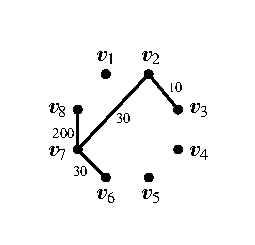
\includegraphics[width=0.33\columnwidth]{fig/example/add_edge_at_5_original.pdf}
			}
			\hspace*{-0.3cm}
			\subfigure[{\scriptsize (Gender)}]{
				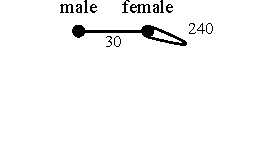
\includegraphics[width=0.33\columnwidth]{fig/example/add_edge_at_5_gender_adjust.pdf}
			}
			\hspace*{-0.3cm}
			\subfigure[{\scriptsize (Gender, Profession)}]{
				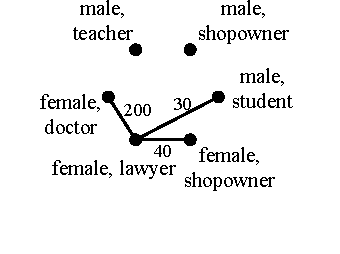
\includegraphics[width=0.33\columnwidth]{fig/example/add_edge_at_5_gender_pro_adjust.pdf}
			}
		\end{tabular}
	\end{center}
	\vspace*{-0.4cm}
	\caption{Snapshots of temp-multi-network in memory at day 5 after a new edge is added}
	\vspace*{-0.4cm}
	\label{fig:add_edge_at_5}
\end{figure}

\begin{figure}[t!]
	\begin{center}
		\begin{tabular}[t]{c}\hspace*{-0.3cm}
			\subfigure[{\scriptsize Original network}]{
				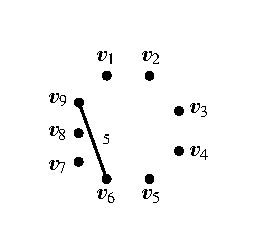
\includegraphics[width=0.33\columnwidth]{fig/example/add_edge_at_6_original.pdf}
			}
			\hspace*{-0.3cm}
			\subfigure[{\scriptsize (Gender)}]{
				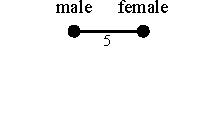
\includegraphics[width=0.31\columnwidth]{fig/example/add_edge_at_6_gender_adjust.pdf}
			}
			\hspace*{-0.3cm}
			\subfigure[{\scriptsize (Gender, Profession)}]{
				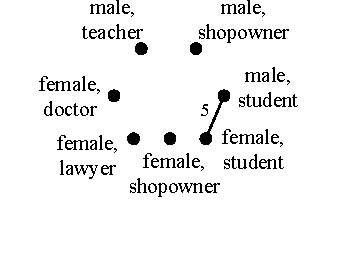
\includegraphics[width=0.33\columnwidth]{fig/example/add_edge_at_6_gender_pro_adjust.pdf}
			}
		\end{tabular}
	\end{center}
	\vspace*{-0.4cm}
	\caption{Snapshots of temp-multi-network in memory at day 6 after a new edge is added}
	\vspace*{-0.4cm}
	\label{fig:add_edge_at_6}
\end{figure}
\begin{example} \label{exam:network_growth}
	Suppose that we need to add two new edges $ e_1=(v_2,v_3,5,10) $ and $ e_2=(v_6,v_9,6,5) $ successively where $ A(v_9)=(female,cn,student) $, $ W(v_9)=800 $ into temporal graph cube built on temp-multi-network in Fig.~\ref{fig:example_dataset} and only two views are precomputed: $ (Gender,\ast,\ast) $ and $ (Gender,\ast,Profession) $. Fig.~\ref{fig:add_edge_at_5} shows the snapshots at day 5 of all temp-multi-networks in the temporal graph cube after $ e_1 $ is added. Since $ v_2 $ and $ v_3 $ are both females, the self loop edge on ``female" in the 5-th snapshot in Fig.~\ref{fig:aggregation_gender} should be updated to the corresponding self loop in Fig.~\ref{fig:add_edge_at_5} (b). Similar update should be performed in the 5-th snapshot in Fig.~\ref{fig:aggregation_gender_profession}, and the result is shown in Fig.~\ref{fig:add_edge_at_5} (c).
	
	When adding $ e_2 $, we need to create new snapshot in each temp-multi-network of the temporal graph cube because $ e_2 $ leads to a new timestamp day 6. For the original network, we create a new snapshot at day 6 as Fig.~\ref{fig:add_edge_at_6} (a) with only $ e_2 $ being stored after all attributes of $ v_9 $ are added into the vertex table of the original temp-multi-network. For other temp-multi-networks of precomputed views, we should also create new snapshots at day 6, holding the aggregated edges of $ e_2 $ as in Fig.~\ref{fig:add_edge_at_6} (b) and (c) after the aggregated vertices of $ v_9 $ are added or updated.
\end{example}
}

%\section{The Proposed Indexes} \label{sec:indexes}
\section{The Index-based Approach}\label{sec:indexes}
In this section, we propose an index-based approach to process the temporal cuboid query (temporal crossboid queries can be transformed to temporal cuboid queries). Recall that for a temporal cuboid query $ Q=(A',[l,r]) $, we need to merge snapshots of a certain temp-multi-network in time range $ [l,r] $ whether $ A' $ is precomputed or not (see lines~8-15 of Algorithm~\ref{alg:temp_cuboid_baseline}). Merging snapshots in time ranges is similar to the classic range query problem: answering online queries $ q=(func,[l,r]) $ on a numeric array $ Arr $, where $ func $ might be SUM($\ast$), AVERAGE($\ast$), MAX($\ast$) or MIN($\ast$), specifying the needed statistical results of values in range $ [l,r] $ of $ Arr $. We can regard merging snapshots in snapshot array as a range query problem on a snapshot array.

\begin{figure}[t!]
	\begin{center}
		\begin{tabular}[t]{c}\hspace*{-0.3cm}
%			\subfigure[{\scriptsize A numeric array}]{
%				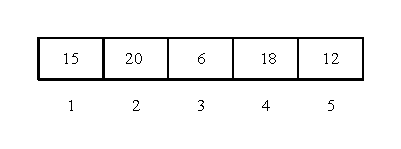
\includegraphics[width=0.85\columnwidth]{fig/example/example_numeric_array_adjust.pdf}
%			}
%			\hspace*{-0.3cm}
%			\\
			\subfigure[{\scriptsize A snapshot array extracted from Fig.~\ref{fig:aggregation_gender_profession}}]{
				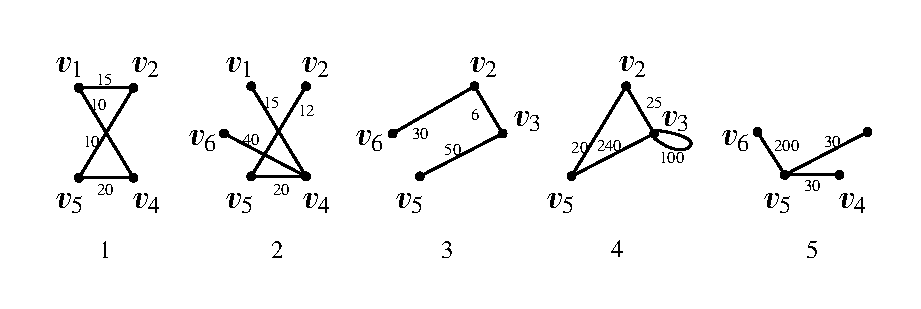
\includegraphics[width=0.7\columnwidth]{fig/example/example_snapshot_array.pdf}
			}
			\hspace*{-0.3cm}
	%		\\
			\subfigure[{\scriptsize Result of range query $ Q $ in Example~\ref{exam:range_query_num_snap_array}}]{
				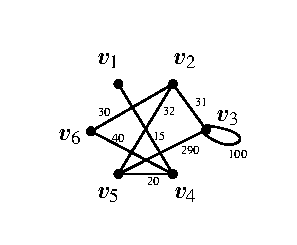
\includegraphics[width=0.25\columnwidth]{fig/example/example_range_query_snapshot.pdf}
			}
		\end{tabular}
	\end{center}
	\vspace*{-0.6cm}
	\caption{Range query on a snapshot array}
	\vspace*{-0.4cm}
	\label{fig:range_query_num_snap_array}
\end{figure}
\begin{example} \label{exam:range_query_num_snap_array}
Fig.~\ref{fig:range_query_num_snap_array} (a) is a snapshot array of temporal aggregate network of precomputed view $ (Gender,\ast,Profession) $ in Fig.~\ref{fig:aggregation_gender_profession}. Here we renumber all vertices and omit the isolated vertices in each snapshot for simplicity. Suppose that a range query on the snapshot array in Fig.~\ref{fig:range_query_num_snap_array} (a) is $ Q=((Gender,\ast,Profession),[2,4]) $ with SUM($\ast$) specified upon edges. We can derive that the result of $ Q $ as shown in Fig.~\ref{fig:range_query_num_snap_array} (b).
\end{example}

%%%%%%%%%
\comment{
Note that there are two differences between the range query on the numeric array and the snapshot array:
\begin{itemize}[leftmargin=*]
	\item We need to merge both the structural information of snapshots and the numeric attributes of edges in snapshots in certain ranges. The range query on the snapshot array can be regarded as the range query on a set array, in which we calculate the union of sets in specified range and maintain the statistical results of numeric attributes on all elements (edges).
	
	\item For the range query on the numeric array, modifying the value at an arbitrary place in the array can be well supported, but updating the size of the array is often hard to support.  However, in temp-multi-network, with the time goes on, the edges will be added into the temp-multi-network. Thus, we need to consider update the size of the array.
\end{itemize}

To address these differences, we propose a segment-tree based index structure to handle the range query in the snapshot array.
}


\comment{
There are many existing methods to build indexes to accelerate range query on the numeric array. In this paper, we implement some representative indexes to accelerate range query on snapshot array and extend them to support self maintenance when new edges are added. Specifically, we divide our problems into two kinds according to aggregation function specified upon edges $ f_e $: 1) $ f_e = $ COUNT($\ast$) or SUM($\ast$). 2) $ f_e= $ MAX($\ast$) or MIN($\ast$). In range query problem on numeric array, if $ func= $ SUM($\ast$) (COUNT($\ast$) is meaningless most of the time) in a query and there is no modification at arbitrary place, we can maintain a simple prefix array $ preArr $, in which
\begin{equation}
	\label{eqt:prearr_range_query}
	preArr[i]=\sum_{j=0}^{j \leq i}Arr[j].
\end{equation}
A query $ q=(func,[l,r]) $ can be easily answered by
\begin{equation}
	\label{eqt:prearr_ans_range_query}
	preArr[r]-preArr[l-1].
\end{equation}
However, if $ func= $ MAX($\ast$) or MIN($\ast$) and we still maintain each $ preArr[i] $ as the maximum (or minimum) of $ Arr $ in $ [0,i] $, we can not tell the maximum (or minimum) in $ [l,r] $ of $ Arr $ if $ preArr[r]=preArr[l-1] $.

It is the same with our problem because range query on numeric array can be regarded as a special case of our problem if each snapshot in snapshot array has only one edge and all edges of those snapshots share the same vertices. As a result, in Section~\ref{subsec:prefix_array}, we briefly discuss how to use prefix array to accelerate temporal cuboid queries when $ f_e $ equals COUNT($\ast$) or SUM($\ast$) and maintain prefix array while new edges are added into the temporal graph cube. In Section~\ref{subsec:sparse_table} and Section~\ref{subsec:segment_tree}, we discuss two different methods to accelerate queries when $ f_e $ equals MAX($\ast$) or MIN($\ast$) and their maintenance while new edges added.

\subsection{Prefix Array} \label{subsec:prefix_array}
Before discussing prefix array, we need to explain that in practical implementation, to support all kinds of aggregation functions we maintain all kinds of statistical results at the same time, i.e., in all snapshots of all temporal aggregate networks of precomputed views, each edge is in form of $ (u,v,c,a,max,min) $ where $ c,a $ are count of edges and amount of attributes respectively.

\stitle{Build.} We can build a prefix array for each precomputed view and $ A_{base} $. The elements in prefix array is still snapshots, but edges in these snapshots are in form of $ (u,v,c,a) $, since we only maintain counts of edges and amounts of numeric attributes of edges using prefix array.
\begin{algorithm}[t]
	\scriptsize
	\caption{$\kw{Build Prefix Array}$}
	\label{alg:build_prefix_array}
	\KwIn{A temp-multi-network $ \Gr=(\Vr,\Sr,A,W) $}
	\KwOut{Prefix Array $ preArray $ for $ \Gr $}
	Let $ preArray $ be an array initialized with $ t_{end}+1 $ empty snapshots;
	
	\ForEach{$ i \in [1,t_{end}] $}{
		$ preArray[i] \gets \Sr[i] $;
	}

	\ForEach{$ i \in [2,t_{end}] $}{
		$ \kw{MergeSnapshotSum}(preArray[i],preArray[i-1]) $;
	}
	\Return $ preArray $;

	\vspace*{0.2cm}
	{\bf Procedure} {$\kw{MergeSnapshotSum}(S_a,S_b)$}
	
	\ForEach{$ e_b \in S_b $}{
		\If{$\exists e_a \in S_a, e_a.u=e_b.u \wedge e_a.v=e_b.v $}{
			$ e_a.c \gets e_a.c+e_b.c $\;
			$ e_a.a \gets e_a.a+e_b.a $;
		}
		\Else{
			$ S_a \gets S_a \cup \{(e_b.u,e_b.v,e_b.c,e_b.a)\} $;
		}
	}
\end{algorithm}

We construct prefix array in Algorithm~\ref{alg:build_prefix_array}. Line~2-5 is the basic process of building a prefix array. The key part in Algorithm~\ref{alg:build_prefix_array} is the \kw{MergeSnapshotSum} procedure, which merges a snapshot $ S_b $ into another snapshot $ S_a $. In detail, for each edge $ e_b $ in $ S_b $, we add $ e_b $ into $ S_a $ (line~13) or update $ e_a $ in $ S_a $ which shares the same vertices with $ e_b $ (line~10-11).

Suppose the summarized snapshot of $ \Gr $ is $ S $, the time complexity and space complexity of Algorithm~\ref{alg:build_prefix_array} are both $ O(t_{end}\times |S|) $.

\stitle{Query.} It is easy to use prefix array to answer $ Q=(A',[l,r]) $ when $ f_e $ is COUNT($\ast$) or SUM($\ast$). Suppose conducting $ Q $ we need merge snapshots in $ [l,r] $ of a temp-multi-network $ \Gr $ ($ \Gr $ may not be the corresponding temporal aggregate network of $ A' $, the reason can be found in Section~\ref{subsec:queries}), and prefix array built for $ \Gr $ is $ preArray $, then the result of merging snapshots of $ \Gr $ can be easily obtained by Algorithm~\ref{alg:prefix_array_query}. If $ A' $ is precomputed, then $ \Gr=\Gr' $ and $ S_E $ (the output of Algorithm~\ref{alg:prefix_array_query}) is the network structure of $ Q $'s result, otherwise the same process in line~17-25 of Algorithm~\ref{alg:temp_cuboid_baseline} should be performed.
\begin{algorithm}[t]
	\scriptsize
	\caption{$\kw{Prefix Array Query}$}
	\label{alg:prefix_array_query}
	\KwIn{Prefix array $ preArray $ for $ \Gr $; Biased time range $ [l,r] $}
	\KwOut{A snapshot $ S_E $, the result of merging snapshots of $ \Gr $ in $ [l,r] $ }
	$ S_E \gets \{\} $;
	$ l \gets l-1 $;
	
	\ForEach{$ e_r \in preArray[r] $}{
		\If{$\exists e_l \in preArray[l], e_r.u=e_l.u \wedge e_r.v=e_l.v $}{
			\lIf{$ e_r.c>e_l.c $}{$ S_E \gets S_E \cup \{(e_r.u,e_r.v,e_r.c-e_l.c,e_r.a-e_l.a)\} $}
		}
		\Else{
			$ S_E \gets S_E \cup \{(e_r.u,e_r.v,e_r.c,e_r.a)\} $;
		}
	}
	\Return $ S_E $;
\end{algorithm}
It is clear that the time complexity of Algorithm~\ref{alg:prefix_array_query} is $ O(|preArray[r]|) $.

\stitle{Update.} We have discussed that there are two situations when adding a new edge $ (u,v,t,a) $: 1) $ t-t_{base}=t_{end} $. 2) $ t-t_{base}>t_{end} $. We directly give the updating algorithm Algorithm~\ref{alg:prefix_array_update}.
\begin{algorithm}[t]
	\scriptsize
	\caption{$\kw{Prefix Array Update}$}
	\label{alg:prefix_array_update}
	\KwIn{Prefix array $ preArray $ for $ \Gr $; Mapped edge $ (u',v',a) $ of new edge $ e=(u,v,t,a) $ used to update $ \Gr $; $ t_{end} $ of $ \Gr $ before $ \Gr $ was updated}
	\KwOut{Updated $ preArray $}
	\If{$ t-t_{base}>t_{end} $}{
		Append $ (t-t_{base}-t_{end}) $ $ preArray[t_{end}] $s to $ preArray $;
	}
	\If{$ \exists e_t \in preArray[t-t_{base}],e_t.u=u' \wedge e_t.v=v' $}{
		$ e_t.c \gets e_t.c+1 $;
		$ e_t.a \gets e_t.a+a $;
	}
	\Else{
		$ preArray[t-t_{base}] \gets preArray[t-t_{base}] \cup \{(u',v',1,a)\} $;
	}
	\Return $ preArray $;
\end{algorithm}

In Algorithm~\ref{alg:prefix_array_update}, the mapped edge $ (u',v',a) $ in the input is used to update $ \Gr $ as we discussed in Section~\ref{subsec:growing}. If $ \Gr $ is the original temp-multi-network, $ (u',v',a)=(u,v,a) $. $ t_{end} $ is the biased timestamp of the latest timestamp in $ \Gr $ before $ \Gr $ was updated. If condition in line~1 is true, then the second situation of adding a new edge is met, and we should extend $ preArray $ to a new length by appending $ (t-t_{base}-t_{end}) $ $ preArray[t_{end}] $s to $ preArray $ (line~2). Whether condition in line~1 is true or false, the last step is updating $ preArray[t-t_{base}] $ with $ (u',v',a) $ (line~3-6).

The time complexity of Algorithm~\ref{alg:prefix_array_update} still depends on situations of adding a new edge. If the first situation is met, the time complexity is $ O(1) $. If the second situation is met, the time complexity is $ O((t-t_{base}-t_{end})\times |preArray[t_{end}]|) $.
}

\comment{
\subsection{Sparse Table} \label{subsec:sparse_table}
Sparse table (STable) is an efficient data structure to accelerate range query on numeric array $ Arr $ with $ O(1) $ time complexity and $ O(nlog(n)) $ space complexity ($ n $ is the length of $ Arr $) only when $ func $ is MAX($\ast$) or MIN($\ast$) in $ q $. If $ func $ is SUM($\ast$), time complexity of conducting $ q $ becomes $ O(log(n)) $. We briefly explain the principle of STable bellow.
\begin{itemize}[leftmargin=*]
	\item For a numeric array $ Arr $ of length $ n $, STable maintains a two-dimensional array $ f $. $ f[i][j] $ represents the maximum (or minimum) in range $ [i-2^j+1,i] $ of $ Arr $.
	
	\item For each query $ q=(func,[l,r]) $, let $ len=r-l+1 $, if $ log(len) $ is an integer, then the answer of $ q $ is $ f[r][log(len)] $. Otherwise, let $ m=\lfloor log(len) \rfloor $, the answer of $ q $ is $ func(f[l+2^m-1][m],f[r][m]) $.
\end{itemize}
When $ log(len) $ is not an integer, we can not use a single element in $ f[r] $ to answer $ q $, but we can use two elements in $ f[l+2^m-1] $ and $ f[r] $, representing two overlapping ranges to answer $ q $. If $ func $ is SUM($\ast$), we can not use the same method to answer $ q $, because in this case, values in overlapping area will be added twice. It doesn't matter if $ func $ is MAX($\ast$) (or MIN($\ast$)), because MAX($ x,x $) still equals $ x $.

For a snapshot $ S $, we can also get MAX($ S,S $) $ =S $, because numeric value $ x $ on each edge of $ S $ still satisfies MAX($ x,x $) $ =x $. Note that the execution of MAX($\ast$) when the parameters are snapshots is similar to \kw{MergeSnapshotExtre} in Algorithm~\ref{alg:stable_build}. Next, we discuss how to extend STable to solve our problem.

First, we switch all elements in $ f $ to snapshots. We first consider the case where $ f_e= $ MAX($\ast$). For a temp-multi-network $ \Gr $ and its snapshot array $ \Sr $, we have
\begin{equation}
	\label{eqt:stable_elements}
	\begin{split}
		f[i][j]=MAX(\Sr[i-2^j+1],\\\Sr[i-2^j+2],...,\Sr[i]).
	\end{split}
\end{equation}
That is, $ f[i][j] $ is the MAX($\ast$) result of snapshots of $ \Sr $ in time range $ [i-2^j+1,i] $.

\stitle{Build.} Building a STable relies on the following equation:
\begin{equation}
	\label{eqt:build_stable}
	f[i][j]=MAX(f[i][j-1],f[i-2^{j-1}][j-1]).
\end{equation}
To support MIN($\ast$), we use edges in form of $ (u,v,max,min) $ in snapshots of $ f $.
\begin{algorithm}[t]
	\scriptsize
	\caption{$\kw{STable Build}$}
	\label{alg:stable_build}
	\KwIn{A temp-multi-network $ \Gr=(\Vr,\Sr,A,W) $}
	\KwOut{STable $ f $ for $ \Gr $}
	Let $ f $ be an array initialized with $ t_{end}+1 $ empty arrays\;
	\ForEach{$ i \in [1,t_{end}] $}{
		$ \kw{BuildSinglePlace}(i,f,\Sr) $;
	}
	\Return $ f $;

	\vspace*{0.2cm}
	{\bf Procedure} {$\kw{MergeSnapshotExtre}(S_a,S_b)$}
	
	\ForEach{$ e_b \in S_b $}{
		\If{$\exists e_a \in S_a, e_a.u=e_b.u \wedge e_a.v=e_b.v $}{
			$ e_a.max \gets MAX(e_a.max,e_b.max) $\;
			$ e_a.min \gets MIN(e_a.min,e_b.min) $;
		}
		\Else{
			$ S_a \gets S_a \cup \{(e_b.u,e_b.v,e_b.max,e_b.min)\} $;
		}
	}

	\vspace*{0.2cm}
	{\bf Procedure} {$\kw{BuildSinglePlace}(pos,f,snapArr)$}
	
	$ f[pos].append(snapArr[pos]) $\;
	$ range \gets 2 $;
	$ i \gets 1 $\;
	\While{$ pos-range+1 \geq 1 $}{
		$ halfRange \gets range>>1 $;
		$ prePos \gets pos-halfRange $\;
		$ f[pos].append(f[pos][i-1]) $\;
		$ \kw{MergeSnapshotExtre}(f[pos][i],f[prePos][i-1]) $\;
		$ range \gets range<<1 $;
		$ i=i+1 $;
	}
\end{algorithm}
Algorithm~\ref{alg:stable_build} is used to build STable for every temp-multi-network.

In line~3 of Algorithm~\ref{alg:stable_build}, \kw{BuildSinglePlace} is executed to build each $ f[i],i\in [1,t_{end}] $. \kw{BuildSinglePlace} procedure is designed based on Equation~\ref{eqt:build_stable} as line~14-19. The key part of Algorithm~\ref{alg:stable_build} is the \kw{MergeSnapshotExtre} procedure, which conducts MAX($\ast$) for snapshots. The time complexity and space complexity of Algorithm~\ref{alg:stable_build} are both $ O(t_{end}\times log(t_{end})|S|) $ where $ S $ is the summarized snapshot of the inputed temp-multi-network.

\stitle{Query.} Algorithm~\ref{alg:stable_query} conducts the range query on snapshot array using STable.
\begin{algorithm}[t]
	\scriptsize
	\caption{$\kw{STable Query}$}
	\label{alg:stable_query}
	\KwIn{STable $ STable $ for $ \Gr $; Biased time range $ [l,r] $}
	\KwOut{A snapshot $ S_E $, the result of merging snapshots of $ \Gr $ in $ [l,r] $}
	$ S_E \gets \{\} $;
	$ range \gets r-l+1 $\;
	$ f \gets STable.f $\;
	\If{$ log(range) $ is an integer}{
		$ S_E \gets f[r][log(range)] $;
	}
	\Else{
		$ logVal \gets \lfloor log(range) \rfloor $\;
		$ S_E \gets f[r][logVal] $\;
		$ powerVal \gets 1<<logVal $\;
		$ \kw{MergeSnapshotExtre}(S_E,f[l+powerVal-1][logVal]) $;
	}

	\Return $ S_E $;
\end{algorithm}
The idea of Algorithm~\ref{alg:stable_query} is similar to algorithms conducting queries on numeric arrays using STable. The only difference is the use of \kw{MergeSnapshotExtre}. The time complexity of Algorithm~\ref{alg:stable_query} is $ O(|S|) $

\stitle{Update.} It is generally considered that STable doesn't support to be updated when modifying at arbitrary places of $ Arr $ in range query problem on numeric array because of the low efficiency. However, in our problem, we only need to modify snapshot array at the last place (i.e., adding a new edge to the last snapshot) or create a new snapshot holding the new edge at the end of the snapshot array. It is possible to update STable in our problem.
\begin{algorithm}[t]
	\scriptsize
	\caption{$\kw{STable Update}$}
	\label{alg:stable_update}
	\KwIn{STable $ STable $ for $ \Gr=(\Vr,\Sr,A,W) $; Mapped edge $ (u',v',a) $ of new edge $ e=(u,v,t,a) $ used to update $ \Gr $; $ t_{end} $ of $ \Gr $ before $ \Gr $ was updated}
	\KwOut{Updated $ STable $}
	$ f \gets STable.f $\;
	\If{$ t-t_{base}>t_{end} $}{
		Append $ (t-t_{base}-t_{end}) $ empty arrays to $ f $;
		
		\ForEach{$ i \in [t_{end}+1,t-t_{base}] $}{
			$ \kw{BuildSinglePlace}(i,f,\Sr) $;
		}
	}
	\Else{
		\ForEach{$ S \in f[t_{end}] $}{
			$ \kw{MergeSnapshotExtre}(S,\{(u',v',a,a)\}) $;
		}
	}
	\Return $ STable $;
\end{algorithm}

We use Algorithm~\ref{alg:stable_update} to update STable. For the second situation of adding new edges, we only need to append $ (t-t_{base}-t_{end}) $ empty 1-D arrays to $ f $ and execute \kw{BuildSinglePlace} at extra places of $ f $ (line~3-5), because the update of STable is later than the update of $ \Gr $ the STable built on, and the process in line~3-5 of Algorithm~\ref{alg:stable_update} can be regarded as a continuing process of line~2-3 in Algorithm~\ref{alg:stable_build}.

The time complexity of Algorithm~\ref{alg:stable_update} still depends on situations of adding a new edge. If situation 1) is met, we should update each snapshot in $ STable.f[t_{end}] $ with mapped edge $ (u',v',a,a) $ (line~7-8), so the time complexity is $ O(log(t_{end})) $. If situation 2) is met, we should conduct \kw{BuildSinglePlace} for $ STable.f[i],i \in [t_{end}+1,t-t_{base}] $, so the time complexity is $ O((t-t_{base}-t_{end})\times log(t-t_{base})|S|) $, $ S $ is the summarized snapshot of $ \Gr $ which STable is built on.

}

\subsection{The Segment Tree Index} \label{subsec:segment_tree}
\comment{
Segment tree (STree) is an efficient data structure to accelerate range query on numeric array, and it supports all kinds of statistical functions mentioned above.
\begin{figure}[t]
	\begin{center}
		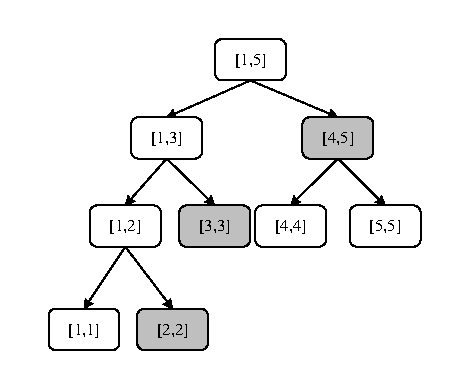
\includegraphics{fig/example/example_segtree.pdf}
	\end{center}
	\vspace*{-0.4cm}
	\caption{An example of STree}
	\vspace*{-0.4cm}
	\label{fig:exam_segtree}
\end{figure}
For example, Fig.~\ref{fig:exam_segtree} shows the structure of STree built for numeric array in Fig.~\ref{fig:range_query_num_snap_array} (a).
}

Here we focus mainly on extending the classic segment tree (STree) structure to support range query on snapshot array when $ f_e $ is MAX($\ast$) or MIN($\ast$) and the maintenance of STree when adding new edges. For the other aggregation functions, including SUM($\ast$) and AVERAGE($\ast$), can be processed in a similar way. Below, we first briefly describe the basic properties of STree.
\begin{enumerate}
	\item STree is a full binary tree, maintaining values for an array. If the length of the array is $ N $, the height of STree is $ \lceil log(N) \rceil+1 $.
	\item Each node in STree maintains statistical result of values in a sub-range of the array. The root of STree maintains the whole range of the array, i.e., $ [1,N] $. The left child and the right child maintain range $ [1,\lfloor(1+N)/2\rfloor] $ and range $ [\lfloor(1+N)/2\rfloor+1,N] $ respectively, which split $ [1,N] $ equally. Both left child and right child can be regarded as roots of sub-STrees and they both have their own childs sharing their ranges equally. The above process for a node ends when its range can not be divided (length equals $ 1 $).
	\item The time complexity of building a STree is $ O(N) $. The space complexity of STree is also $ O(N) $. The time complexity of processing a query $ q=(func,[l,r]) $ is $ O(log(N)) $.
\end{enumerate}

Unlike traditional range query problem, there are two differences in our range query problem: 1) elements in the array and statistical results in nodes of STree are not numeric values but snapshots, with edges in form of $ (u,v,max,min) $; and 2) the range of STree might be expanded because of inserting new edges. Merging statistical information of nodes is a basic and frequent operation in both building and querying of STree, in which two statistical results of two nodes produce a new result. For the first difference, all we need to do is replacing the original operation on numeric values with \kw{MergeSnapshotExtre} procedure (see Algorithm~\ref{alg:stree_query}). We will address the second difference in the \stitle{Update} algorithm (see Algorithm~\ref{alg:update_stree}).  Below, we first briefly describe the index building procedure, followed by the query processing procedure and index updating procedure.

\stitle{STree building.} We omit the detailed algorithm to build the STree for a snapshot array, because we only need to replace the merging operation of two numeric values in the traditional algorithm of building STree for numeric array with the proposed \kw{MergeSnapshotExtre} procedure  (see Algorithm~\ref{alg:stree_query}). For example, Fig.~\ref{fig:exam_segtree} illustrates a STree $ STree $ for the snapshot array in Fig.~\ref{fig:range_query_num_snap_array}. Note that each node of $ STree $ maintains a snapshot. Fig.~\ref{fig:exam_stree_node} shows the snapshot of the node $ [1,3] $ of $ STree $ in Fig.~\ref{fig:exam_segtree}.



\begin{figure}[t]
	\begin{center}
		\begin{tabular}[t]{c}\hspace*{-0.3cm}
\subfigure[{\scriptsize The STree}]{
				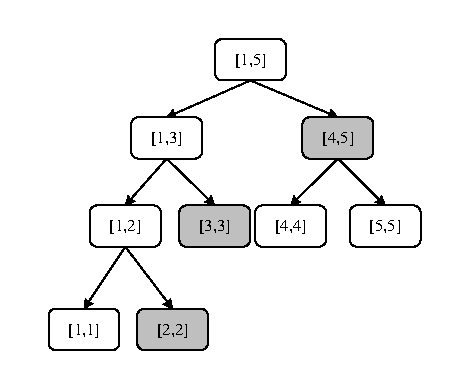
\includegraphics[width=0.5\columnwidth, height=3cm]{fig/example/example_segtree.pdf} \label{fig:exam_segtree}
			} %\hspace*{-0.3cm}
\subfigure[{\scriptsize Snapshot in the node $ [1,3] $}]{
				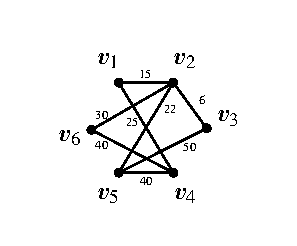
\includegraphics[width=0.4\columnwidth]{fig/example/example_stree_node_1_3.pdf} 	\label{fig:exam_stree_node}
			}
\end{tabular}
	\end{center}
	\vspace*{-0.6cm}
	\caption{A STree built on the snapshot array in Fig.~\ref{fig:range_query_num_snap_array}}
	\vspace*{-0.6cm}
	\label{fig:stree}
\end{figure}

As we have mentioned before, the time complexity for building a traditional STree is $ O(N) $. Since \kw{MergeSnapshotExtre} will be called in building each node, the time complexity of building STree for snapshot array of length $ N $ is $ O(N|S|) $, where $ S $ is the summarized snapshot of the snapshot array. Also, it is easy to derive that the space usage of the STree building procedure is  $ O(N|S|) $.

%The space consumed by STree built for the snapshot array is also $ O(N|S|) $. Note that each node $ node $ in STree is a struct, where $ node.lchild $ and $ node.rchild $ are left child and right child of $ node $ respectively and $ [node.timel,node.timer] $ is the range which $ node $ maintains. For leaves of STree, $ lchild $ and $ rchild $ are $ NULL $. Suppose the snapshot array STree built on is $ \Sr $, $ node.snapshot $ can be regarded as the summarized snapshot of snapshot sub-array $ [\Sr[node.timel-t_{base}],...,\Sr[node.timer-t_{base}]] $. STree $ STree $ is also a struct, where $ STree.root $ is the root of $ STree $.

\stitle{Query processing.} Algorithm~\ref{alg:stree_query} conducts the range query on snapshot array using STree, and it shares the same framework with original query algorithm on STree but uses \kw{MergeSnapshotExtre} to merge snapshots. Merging snapshots only happens when the current split range $ [timel,timer] $ equals the range held by the current node $ treeNode $ (line~2 in Algorithm~\ref{alg:stree_query}). In the worst case, it happens at each depth of STree, so the time complexity of Algorithm~\ref{alg:stree_query} is $ O(log(N)|S|) $. For example, suppose we conduct a query $ Q=(\ast,[2,5]) $ on snapshot array in Fig.~\ref{fig:range_query_num_snap_array} (a) (the view in $ Q $ is omitted), we have to merge snapshots in nodes with range $ [2,2] $, $ [3,3] $ and $ [4,5] $ as in grey nodes in Fig.~\ref{fig:exam_segtree}.
\begin{algorithm}[t]
	\scriptsize
	\caption{$\kw{STreeQuery(treeNode,timel,timer,ans)}$}
	\label{alg:stree_query}
	\KwIn{$ treeNode $, node to be visited; Time range $ [timel,timer] $; $ ans $, a snapshot holding the current result}
	\lIf{$ treeNode=NULL $}{\Return}
	\If{$ timel=treeNode.timel \wedge timer=treeNode.timer $}{
		$\kw{MergeSnapshotExtre}(ans,treeNode.snapshot)$\;
		\Return;
	}
	$ mid \gets (treeNode.timel+treeNode.timer)/2 $\;
	\lIf{$ timel > mid $}{$ STreeQuery(treeNode.rchild,timel,timer,ans) $}
	\lElseIf{$ timer \leq mid $}{$ STreeQuery(treeNode.lchild,timel,timer,ans) $}
	\Else{
		$ STreeQuery(treeNode.lchild,timel,mid,ans) $\;
		$ STreeQuery(treeNode.rchild,mid+1,timer,ans) $;
	}

\vspace*{0.2cm}
	{\bf Procedure} {$\kw{MergeSnapshotExtre}(S_a,S_b)$}
	
	\ForEach{$ e_b \in S_b $}{
		\If{$\exists e_a \in S_a, e_a.u=e_b.u \wedge e_a.v=e_b.v $}{
			$ e_a.max \gets MAX(e_a.max,e_b.max) $\;
			$ e_a.min \gets MIN(e_a.min,e_b.min) $;
		}
		\Else{
			$ S_a \gets S_a \cup \{(e_b.u,e_b.v,e_b.max,e_b.min)\} $;
		}
	}
	\Return;
\end{algorithm}

\stitle{Index updating.} Let $ STree.root.timer $ be the current largest timestamp in the STree. When a new edge $ (u,v,t,a) $ with $t>STree.root.timer $ comes, we need to expand the range of STree by creating new nodes to maintain larger range and switch the root of STree to one of the new nodes.

%The largest timestamp that STree maintains is $ STree.root.timer $, so the two cases in updating STree when adding a new edge $ (u,v,t,a) $ are: 1) $ t \leq STree.root.timer $. 2) $ t>STree.root.timer $. If case 2) is met, we need to expand the range of STree by creating new nodes to maintain larger range and switch the root of STree to one of the new nodes.

Suppose that $ l=STree.root.timel,r=STree.root.timer $, if $ t>r $, we first create a new node $ newNode $ with range $ [l,2r-l+1] $, which is twice the length of $ [l,r] $, so that $ STree.root $ can be a valid left child of $ newNode $. Then, we let $ STree.root $ be the left child of $ newNode $. Finally, we let $ newNode $ be the new root of $ STree $. If $ [l,2r-l+1] $ still can not cover $ t $, we continue the process above until $ t $ is coverd. The updated $ STree $ is not a fully binary tree, since there is only a left subtree for the new root which violates the basic properties of STree. However, it can be seen as a part of a standard STree, which might be completed by continuously added new edges.

\comment{
\begin{figure}[t]
	\begin{center}
		\begin{tabular}[t]{c}\hspace*{-0.3cm}
			\subfigure[{\scriptsize Expanded STree waiting for the new edge}]{
				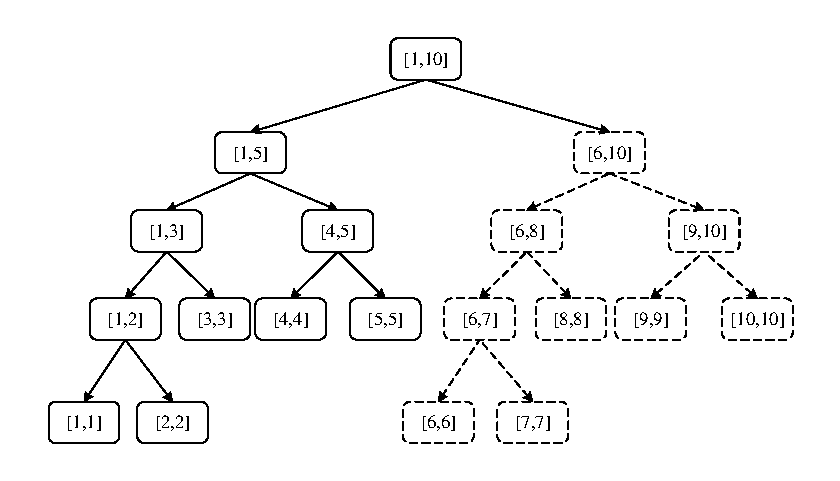
\includegraphics[width=0.75\columnwidth, height=3cm]{fig/example/example_segtree_expand.pdf}
			}
			\hspace*{-0.3cm}
			\\
			\subfigure[{\scriptsize Expanded STree being inserted with a new edge}]{
				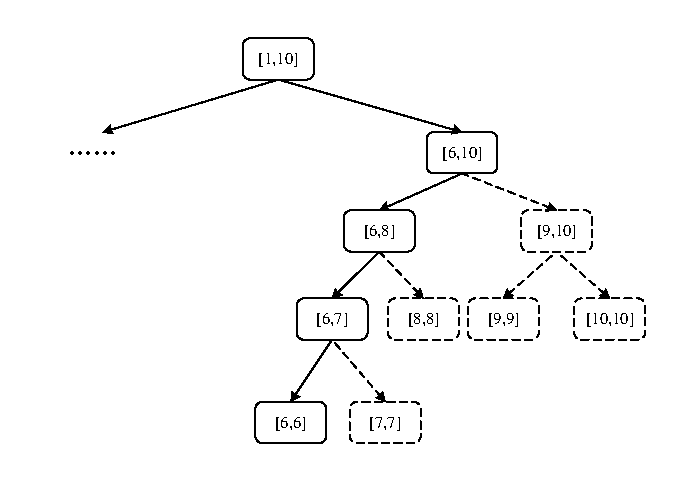
\includegraphics[width=0.75\columnwidth, height=3cm]{fig/example/example_segtree_expand_inserted.pdf}
			}
		\end{tabular}
	\end{center}
	\vspace*{-0.4cm}
	\caption{Update STree when new edges are added}
	\vspace*{-0.4cm}
	\label{fig:exam_segtree_expand}
\end{figure}
\begin{example} \label{exam:stree_expand}
	Suppose we have built a STree $ STree $ for snapshot array in Fig.~\ref{fig:range_query_num_snap_array} (a) and $ STree.root.timer=5 $. If we want to add the new edge $ e_2 $ with timestamp 6, we should update $ STree $ so that it can cover $ [1,6] $. The updated $ STree $ is shown in Fig.~\ref{fig:exam_segtree_expand} (a), where we create a new node $ newNode $ with range $ [1,10] $ and let $ STree.root $ be the $ lchild $ of $ newNode $. Finally we assign $ newNode $ to be the new root of $ STree $. The updated $ STree $ without the nodes presented by dotted rectangles in Fig.~\ref{fig:exam_segtree_expand} (a) is not a complete STree. As shown in Fig.~\ref{fig:exam_segtree_expand} (b) (we omit the left subtree of the root for simplicity), only nodes on path from the root to leaf with range $ [6,6] $ are needed to maintain the aggregated edge of $ e_2 $, so we only need to create or update nodes on that path.
\end{example}
}

\begin{algorithm}[t]
	\scriptsize
	\caption{$\kw{UpdateSTree}$}
	\label{alg:update_stree}
	\KwIn{STree $ STree $ built for $ \Gr $; Mapped edge $ (u',v',a) $ of new edge $ e=(u,v,t,a) $ used to update $ \Gr $;}
	\KwOut{Updated STree $ STree $}
	\While{$ STree.root.timer<t $}{
		$ newRoot \gets $ a new empty STree node\;
		$ newRoot.timel \gets STree.root.timel $\;
		$ newRoot.timer \gets 2 \times STree.root.timer+1-STree.root.timel $\;
		$ newRoot.lchild \gets STree.root $\;
		$ newRoot.snapshot \gets STree.root.snapshot $\;
		$ STree.root \gets newRoot $;
	}
	$\kw{STreeInsertEdge}(STree.root,(u',v',t,a))$;
	
	\Return $ STree $;

	\vspace*{0.2cm}
	{\bf Procedure} {$\kw{STreeInsertEdge}(treeNode,e'=(u',v',t,a))$}
	
	$ \kw{MergeSnapshotExtre}(treeNode.snapshot,\{(u',v',a,a)\}) $;
	
	\lIf{$ treeNode.timel=treeNode.timer $}{\Return}
	$ mid \gets \lfloor(treeNode.timel+treeNode.timer)/2\rfloor $\;
	\If{$ t \leq mid $}{
		\If{$ treeNode.lchild=NULL $}{
			$ newNode \gets $ a new empty STree node\;
			$ treeNode.lchild \gets newNode $\;
			$ newNode.timel \gets treeNode.timel $\;
			$ newNode.timer \gets mid $;
		}
		$\kw{STreeInsertEdge}(treeNode.lchild,e')$;
	}
	\Else{
		\If{$ treeNode.rchild=NULL $}{
			$ newNode \gets $ a new empty STree node\;
			$ treeNode.rchild \gets newNode $\;
			$ newNode.timel \gets mid+1 $\;
			$ newNode.timer \gets treeNode.timer $;
		}
		$ \kw{STreeInsertEdge}(treeNode.rchild,e') $;
	}
\end{algorithm}

Algorithm~\ref{alg:update_stree} is used to update STree. In line~1, the condition in the while loop is true which means that the current root of $ STree $ can not cover $ t $. So, we need to create a new root, which has a double size of range compared to the current root (line~3-4). In line~6, we directly copy the snapshot of the current root to the new root, since there is no possible right child for the new root before new edge is added. If the range of the candidate new root can not cover $ t $ (it hardly happens because of the density of timestamps in real-word large scale temporal network), then the loop in line~1 continues. When $ STree.root.timer \geq t $ is true, we can use \kw{STreeInsertEdge} procedure to update STree. In line~11, we update the snapshot of $ treeNode $ with the mapped edge, since $ t $ is in $ [treeNode.timel,treeNode.timer] $. In line~15 and line~22, we need to test whether the left child or the right child exists or not and create left child (lines~16-19) or right child (lines~23-26). %We have discussed the reason before, that the STree is not complete after being expanded to maintain a larger range.

The time complexity of Algorithm~\ref{alg:update_stree} contains two parts: creating new root in lines~1-7 and inserting new edge using \kw{STreeInsertEdge} procedure. Suppose the length of range maintained by the root of STree is $ len_1=STree.root.timer-STree.root.timel+1 $ before new edge is added, and the length of new range of timestamps in $ \Gr $ becomes $ len_2=t-STree.root.timel+1 $ after $ \Gr $ is updated. To cover $ len_2 $, we need repeat the loop in line~1 at least $ x $ times, and we have
\begin{equation}
	\label{eqt:new_root_create_times}
%	\begin{split}
		len_1*2^x \geq len_2, \quad
		x \geq log(\frac{len_2}{len_1}).
%	\end{split}
\end{equation}
For each loop, the cost mainly comes from line~6. Suppose that the snapshot maintained in root is $ S_{root} $ before a new edge is added, the time complexity of creating the new root is $ O(log(\frac{len_2}{len_1})\times |S_{root}|) $. In practice, $ len_2>len_1 $ is hardly true because $ len_1 $, the length of range maintained by root, grows exponentially (lines~3-4) but $ len_2 $ grows linearly since timestamps in real-world temporal graph are dense. In \kw{STreeInsertEdge} procedure, let the length of range in the final new root is $ len $, the procedure go through the $ log(len)+1 $ layers of STree, in each layer it updates the snapshot of node covering $ t $ or creates necessary node first. Since updating a snapshot and creating a new empty node both contain a constant number of operations, the time complexity of \kw{STreeInsertEdge} procedure is $ O(log(len)+1) $.

\section{Effectiveness of the Index} \label{sec:effec_of_indexes}
In traditional range query problems, indexes are helpful to accelerate the query processing. However, similar indexes cannot always work in our problem, since the elements in the array are not numeric values but snapshots.

\begin{figure}[t] %\vspace*{-0.5cm}
	\begin{center}
		\begin{tabular}[t]{c}\hspace*{-0.3cm}
			\subfigure[{\scriptsize }]{
				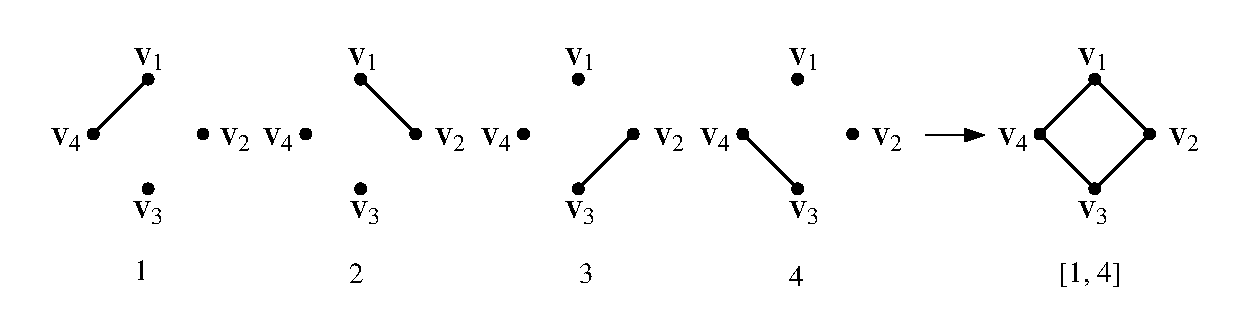
\includegraphics[width=0.95\columnwidth]{fig/example/example_index_fail.pdf}
			}
			\hspace*{-0.3cm}
			\\
			\subfigure[{\scriptsize }]{
				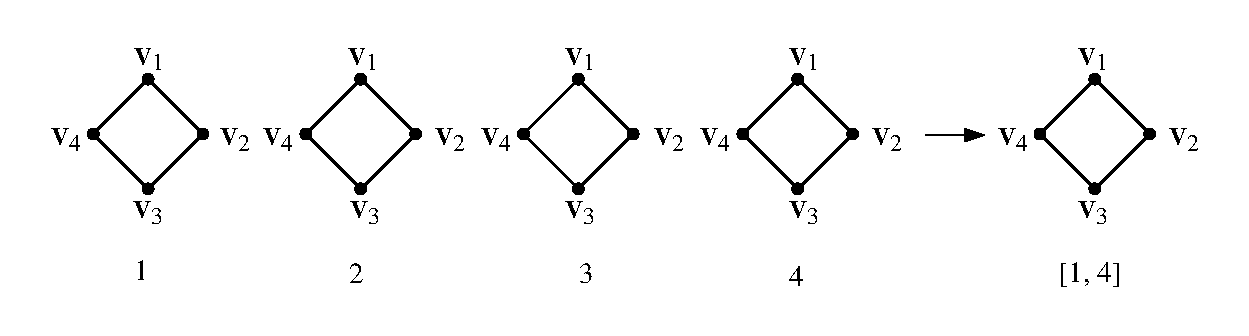
\includegraphics[width=0.95\columnwidth]{fig/example/example_index_success.pdf}
			}
		\end{tabular}
	\vspace*{-0.3cm}
		\caption{Two cases of range query on snapshot array}
		\vspace*{-0.6cm}
		\label{fig:index_fail_success_example}
	\end{center}
\end{figure}
Consider an example in Fig.~\ref{fig:index_fail_success_example} (a), there is no single edge shared by any two snapshots (edge $ e $ is shared by snapshots means that there exists an edge that share the vertices with $ e $ in each of those snapshots). In this case, if we merge snapshots in $ [t_1,t_4] $, the best choice is the baseline method, i.e., traversing all snapshots in the range and computing the result one by one. In baseline method, only $ 4 $ edges will be visited and each of them is visited only once. The edges in the result (snapshot at the right of the arrow in Fig.~\ref{fig:index_fail_success_example} (a)) are exactly those $ 4 $ edges, thus the baseline method achieves the highest efficiency and there is no need to build indexes in this case.

Consider the second example in Fig.~\ref{fig:index_fail_success_example} (b), all snapshots share the same edges. In this case, if we still merge snapshots in $ [t_1,t_4] $, each edge will be visited $ 4 $ times in the baseline method, therefore it is necessary to build index. Next, we describe the measurement of the necessity of index and the key factor we found which affects the necessity of index.
\begin{definition}[Acceleration Ratio of Index]
	\label{def:acceleration_ratio_index}
	For an array $ Arr $ with numeric values or snapshots, we build a segment tree index on it. For a query $ q=(func,[l,r]) $, assume that the basic components are visited $ C_b $ times using the baseline method and $ C_i $ times using the index-based method, the acceleration ratio of the index on $ q $ is $ \frac{C_b}{C_i} $.
\end{definition}
The basic components in snapshot array and index built on snapshot array are edges. We use the number of visited edges as the measure of time consumption when conducting a query using the baseline method and using the index-based method in Definition~\ref{def:acceleration_ratio_index}.
\begin{definition}[Similarity of Snapshots]
	\label{def:similarity_snapshots}
	Given a snapshot array $ snapArr $ starting from $ 1 $ and containing $ n $ snapshots, the summarized snapshot $ S $ of all snapshots in $ snapArr $, $ E=\sum_{i=1}^{n}|snapArr[i]| $, the similarity of snapshots in $ snapArr $ is $ s=\frac{E}{|S|} $.
\end{definition}
In other words, the similarity of snapshots is the ratio of the total number of edges in snapshot array to the size of the summarized snapshot. For simplicity, we assume that each snapshot in $ snapArr $ has at least one edge. Clearly, for a snapshot array of length $ n $, similarity of snapshots $ s $ is in $ [1,n] $.
\begin{example}
	Consider examples in Fig.~\ref{fig:similarity}.
	\begin{figure}[t] %\vspace*{-0.5cm}
		\begin{center}
			\begin{tabular}[t]{c}\hspace*{-0.3cm}
				\subfigure[{\scriptsize $ s=1 $}]{
					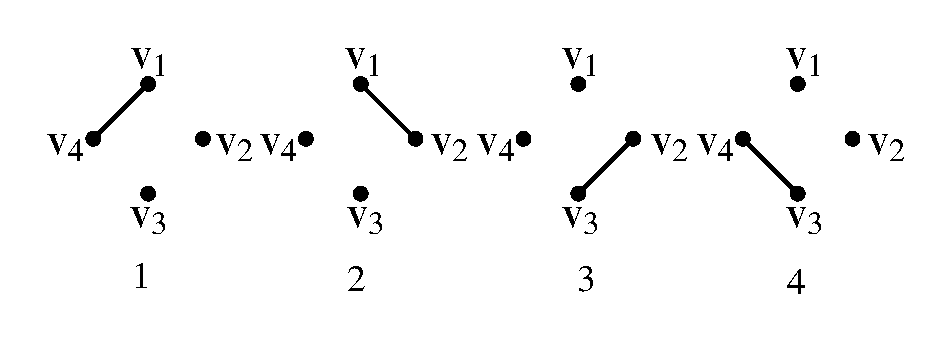
\includegraphics[width=0.5\columnwidth]{fig/example/example_similarity_a.pdf}
				}
				\hspace*{-0.5cm}
				\subfigure[{\scriptsize $ s=4 $}]{
					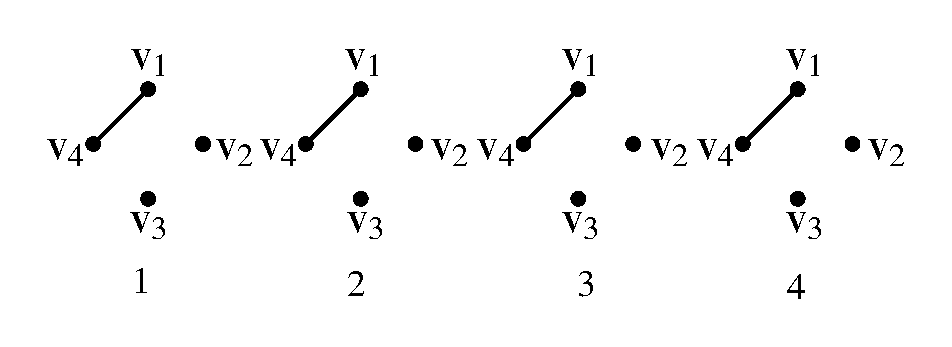
\includegraphics[width=0.5\columnwidth]{fig/example/example_similarity_b.pdf}
				}
				\\
				\subfigure[{\scriptsize $ s=\frac{5}{3} $}]{
					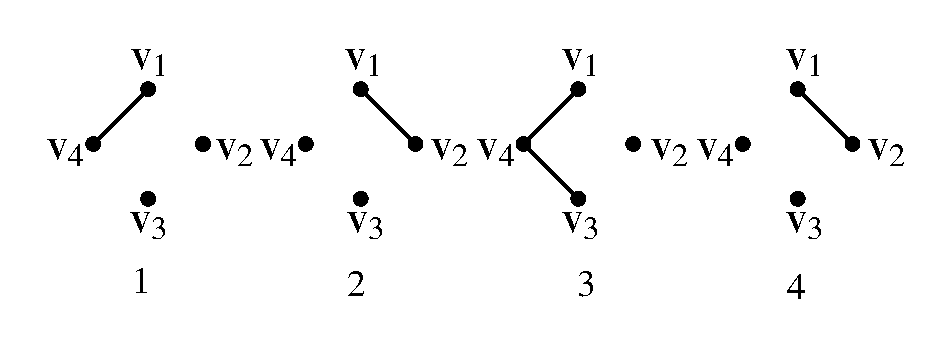
\includegraphics[width=0.5\columnwidth]{fig/example/example_similarity_c.pdf}
				}
				\hspace*{-0.5cm}
				\subfigure[{\scriptsize $ s=4 $}]{
					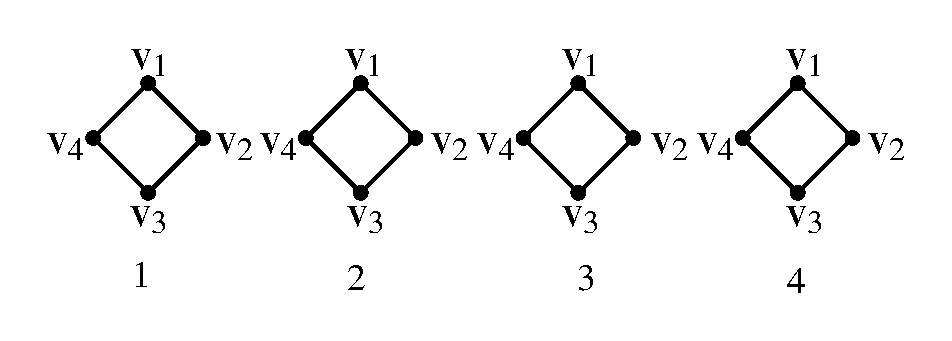
\includegraphics[width=0.5\columnwidth]{fig/example/example_similarity_d.pdf}
				}
			\end{tabular}
			\vspace*{-0.5cm}
			\caption{Four snapshot arrays with different similarity of snapshots}
			\vspace*{-0.8cm}
			\label{fig:similarity}
		\end{center}
	\end{figure}
	There are 4 snapshot arrays having the same length of 4 but different similarities of snapshots $ s $. In Fig.~\ref{fig:similarity} (a), $ s=1 $, and we can see that there is no edge shared by any two snapshots, or, snapshots in Fig.~\ref{fig:similarity} (a) are not similar to each other. In Fig.~\ref{fig:similarity} (b) and (d), $ s=4 $, all snapshots share the same edges. In Fig.~\ref{fig:similarity} (c), $ s=\frac{5}{3} $, and there are edges shared by some snapshots.
\end{example}
From the above examples, we can see that with the similarity of snapshots grows, there will be more snapshots in snapshot array which are similar to each other, or, more edges are shared by snapshots.

\begin{theorem}
	\label{thm:best_index_efficiency}
	For two arrays of length $ n $ and starting from $ 1 $, snapshot array $ snapArr $ and numeric array $ numArr $, if similarity of snapshots in $ snapArr $ equals $ n $, then for any query $ q=(func,[l,r]) $ on both $ snapArr $ and $ numArr $, the acceleration ratios of the same index built on them are equal.
\end{theorem}
\comment{
\begin{proof}
	In Section~\ref{sec:indexes}, we know that the elements in all indexes built on snapshot array are snapshots, which can be regarded as summarized snapshots of different snapshot sub-arrays of the original snapshot array. If the similarity of snapshots in $ snapArr $ is $ n $, then all snapshots in $ snapArr $, as well as their summarized snapshot, share the same edges. It is clear that all snapshots in indexes also share the same edges with snapshots in $ snapArr $. Suppose the indexes built on $ snapArr $ and $ numArr $ are two STrees $ snapSTree $ and $ numSTree $ (the proofs on prefix array and STable are simple, so we only analyse STree here), and summarized snapshot of snapshots in $ snapArr $ is $ S $. In baseline method, conducting $ q $ requires $ r-l+1 $ visits on numeric values in $ numArr $ and $ (r-l+1)|S| $ visits on edges in $ snapArr $. In STree, the structures of $ snapSTree $ and $ numSTree $ are the same, because the structure of STree is only related to the entire range of the array maintained by STree, and nodes where merging happens in $ snapSTree $ and $ numSTree $ (when condition in line~2 of Algorithm~\ref{alg:stree_query} is true) correspond one by one, because the ways that $ [l,r] $ in $ q $ split are the same in $ snapSTree $ and $ numSTree $. If there are $ C_n $ nodes being merged in $ numSTree $, then there are $ C_n $ nodes being merged in $ snapSTree $ and $ C_n|S| $ edges being visited. Thus, the acceleration ratio of $ snapSTree $ ($ \frac{(r-l+1)|S|}{C_n|S|} $) is equal to that of $ numSTree $ ($ \frac{r-l+1}{C_n} $).
\end{proof}
}
\begin{theorem}
	\label{thm:worst_index_efficiency}
	For a snapshot array $ snapArr $ of length $ n $ and starting from 1. If similarity of snapshots in $ snapArr $ equals 1, then for query $ q=(func,[l,r]) $ on $ snapArr $, the acceleration ratio of STree is less than or equal to 1.
\end{theorem}
\comment{
\begin{proof}
	Suppose $ l,r $ are biased timestamps. Since the similarity of snapshots in $ snapArr $ is 1, there is no edge shared by any snapshots in $ snapArr $, e.g., snapshot array in Fig.~\ref{fig:index_fail_success_example} (a). For any summarized snapshot $ S_{ij} $ of sub-array $ [snapArr[i],snapArr[i+1],...,snapArr[j]] $, we can easily get $ |S_{ij}|=\sum_{k=i}^{j}|snapArr[k]| $. For STree $ snapSTree $ built for $ snapArr $ (time range in $ q $ should be $ [l+t_{base},r+t_{base}] $ when using STree, and the proof on STable is simple so we omit it here), suppose the set of nodes being merged in conducting $ q $ is $ NS $, we can easily get $ \sum_{node \in NS}|node.snapshot|=\sum_{k=l}^{r}|snapArr[k]| $, where $ \forall node \in NS,|node.snapshot|=\sum_{k=node.timel}^{node.timer}|snapArr[k-t_{base}]| $. As a result, in query functions of baseline method and STree, we must visit the same number of edges. Considering the cost of visiting nodes in STree, the acceleration ratio of STree is less than or equal to 1. For prefix array $ preArray $ built for $ snapArr $, as in Algorithm~\ref{alg:prefix_array_query}, the number of edges being visited in conducting $ q $ is $ |preArray[r]|=\sum_{k=1}^{r}|snapArr[k]| $. Thus, the acceleration ratio of prefix array is $ \frac{\sum_{k=l}^{r}|snapArr[k]|}{\sum_{k=1}^{r}|snapArr[k]|} $.
\end{proof}
}

The above two theorems show the necessity of building index in two extreme cases. As in Theorem~\ref{thm:best_index_efficiency}, if similarity of snapshots in snapshot array equals the length of the snapshot array, the index-based solution achieves the designed acceleration ratio as they perform in range query on numeric arrays. As in Theorem~\ref{thm:worst_index_efficiency}, if similarity of snapshots in snapshot array equals 1, STree has no acceleration effect. The baseline method is the best approach to conduct any query in this case, because the number of edges in the result is exactly the number of edges being visited in the baseline method.

It is difficult to model the relationship between similarity of snapshots and acceleration ratio of the index-based solution on all possible queries precisely, because similarity of snapshots describes the overall similarity of snapshots in the snapshot array, but in specific queries, snapshots in sub-arrays specified by ranges of the queries may not show the same similarity as the overall similarity. However, it is possible to model the relationship roughly. If the similarity of snapshots in snapshot array equals 1, there is no edge shared by two snapshots and visited more than once in baseline method. If the similarity of snapshots in snapshot array equals the length of the array, all edges are shared by all snapshots. In this case, each edge will be visited repeatedly in each cycle of baseline method (line~8 in Algorithm~\ref{alg:temp_cuboid_baseline}), while the index stores summarized snapshots of some sub-arrays of the snapshot array in advance to reduce the number of repeated visits on edges. With the similarity of snapshots grows from 1 to the length of snapshot array, more edges will be shared by snapshots, making the efficiency of baseline method lower and efficiency of indexes higher. As a result, the acceleration ratio of the index grows when similarity of snapshots grows, which will be confirmed in our experiments in Section~\ref{subsec:efficiency_eva}.

The similarity of snapshots also affects the space consumption of the index. Since the elements in all snapshot arrays and the STree built on them are snapshots, we use the total number of edges in all snapshots to indicate the space consumption. For example, if we build two STrees $ STree_a $ and $ STree_b $ on both snapshot arrays in Fig.~\ref{fig:similarity} (a) and (b), the snapshot in each node of $ STree_b $ has only one edge, while the snapshot in each node of $ STree_a $ may have to store more than one edge, even if Fig.~\ref{fig:similarity} (a) and (b) have the same number of edges.

\begin{definition}[Space Consumption Ratio]
	\label{def:space_consum_ratio}
	Consider an array $ Arr $ holding numeric values or snapshots. If $ Arr $ is a snapshot array, suppose the total number of edges in $ Arr $ is $ E_a $, and the total number of edges in the index is $ E_i $. If $ Arr $ is a numeric array, $ E_a,E_i $ are the total number of numeric values in $ Arr $ and in the index respectively. The space consumption ratio of the index is $ \frac{E_i}{E_a} $.
\end{definition}
\begin{theorem}\label{thm:best_index_space_ratio}
	For two arrays of length $ n $ and starting from 1, snapshot array $ snapArr $ and numeric array $ numArr $, if similarity of snapshots in $ snapArr $ equals $ n $, then the space consumption ratios of the same index built on the two arrays are equal.
\end{theorem}
\comment{
\begin{proof}
	We mentioned that in proof of Theorem~\ref{thm:best_index_efficiency}, the structures of STree built on $ numArr $ and $ snapArr $ are the same. It is the same with the array structure of prefix array and STable. We can turn indexes into sets holding elements like: $ (SumElement,[l,r]) $, and if an index is built on $ numArr $, $ SumElement $ is the aggregation result of numeric values in $ [l,r] $, otherwise the summarized snapshot of snapshots in $ [l,r] $. For each index, suppose we build the index on $ numArr $ and $ snapArr $, named $ numIndex $ and $ snapIndex $. There must be a bijection between elements in $ numIndex $ and $ snapIndex $ that for each $ i $ in $ numIndex $, there is a corresponding $ j $ in $ snapIndex $ that $ i $ and $ j $ have the same time range $ [l,r] $, since the structures of $ numIndex $ and $ snapIndex $ are the same. It is easy to know that the space consumption ratio of $ numIndex $ is $ \frac{|numIndex|}{n} $. Since the similarity of snapshots in $ snapArr $ is $ n $, all snapshots in $ snapArr $ and $ snapIndex $ share the same edges. Suppose the summarized snapshot of snapshots in $ snapArr $ is $ S $, the space consumption ratio of $ snapIndex $ is $ \frac{|snapIndex||S|}{n|S|} $, since $ |snapIndex|=|numIndex| $, so the space consumption ratio of $ snapIndex $ and $ numIndex $ are equal.
\end{proof}
}

Similar to the acceleration ratio, the space consumption ratio of the index is also negatively affected by the decrease of similarity of snapshots. %Specifically, we discuss the space consumption ratio of STree if similarity of snapshots equals 1.
\begin{theorem}\label{thm:stree_worst_index_space_ratio}
	For a snapshot array $ snapArr $ of length $ n $ and starting from 1. If similarity of snapshots in $ snapArr $ equals 1, the space consumption ratio of STree built on $ snapArr $ is in $ (\lceil log(n) \rceil,\lceil log(n) \rceil+1] $.
\end{theorem}
\comment{
\begin{proof}
	Let $ m=\sum_{i=1}^{n}|snapArr[i]| $. If $ log(n) $ is an integer, the height of STree built on $ snapArr $ is $ log(n)+1 $. Consider the $ (log(n)+1) $-th layer of STree, all nodes on the $ (log(n)+1) $-th layer of STree are leaves. It is clear that the total number of edges in snapshots of the leaves is $ m $. For each node on the $ log(n) $-th layer, the snapshot in the node is the summarized snapshot of snapshots in the two siblings of the node. Since the similarity of snapshots in $ snapArr $ is 1, no edge is shared by snapshots in $ snapArr $, so the size of snapshot of each node on the $ log(n) $-th layer is the sum of the size of snapshots in the two siblings. Thus, the total number of edges in snapshots of nodes on the $ log(n) $-th layer is still $ m $. It is the same for nodes on each layer. Finally, the total number of edges in snapshots of all nodes in STree is $ (log(n)+1)\times m $, so the space consumption ratio of STree is $ log(n)+1 $.
	
	If $ log(n) $ is not an integer, then the number of leaves on the $(\lceil log(n) \rceil +1)$-th layer is less than $ n $, so there are less than $ m $ edges on the $(\lceil log(n) \rceil +1)$-th layer, but still $ m $ edges on other layers. Thus, the total number of edges in STree is in $ (\lceil log(n) \rceil\times m, (\lceil log(n) \rceil+1)\times m) $. As a result, in this case, the space consumption ratio of STree is in $ (\lceil log(n) \rceil , \lceil log(n) \rceil+1) $.
\end{proof}
}

From Theorem~\ref{thm:stree_worst_index_space_ratio}, if similarity of snapshots equals 1, we need more space to store STree, which may be $ log(n)+1 $ times the space of the original snapshot array, while only 2 times the space is needed to store STree if similarity of snapshots equals the length of the original snapshot array. %For prefix array and STable, it is impossible to derive a clear mathematical expression of the space consumption ratio related to $ n $ only. But similar to STree, with the decrease of similarity of snapshots, each snapshot in indexes has to store more edges even if the number of edges in its corresponding sub-array of the original snapshot array remains the same. We will prove the above findings in experiment of Section~\ref{subsec:efficiency_eva}.

Based on the above analysis, we can conclude that the necessity of building indexes, which can be determined by acceleration ratio and space consumption ratio of indexes, varies with the similarity of snapshots. This is the main difference of range query on a snapshot array compared to range query on a numeric array. Based on this observation, it is better to build index on the snapshot array with high similarity of snapshots. This is compatible with the implementation strategy of \kw{Temporal\enspace Graph\enspace Cube} presented in the next section, which requires precomputing views with high similarity of snapshots in their snapshot arrays.
%In particular, we use, we know that if similarity of snapshots $ s $ equals $ 1 $, baseline method is the best method and there is no need to build indexes. If $ s $ equals the length of the snapshot array, indexes achieve the designed acceleration ratio, so it is necessary to build indexes just like what we usually do in common range query problem. However, in real-world temp-multi-networks and their precomputed temp-aggre-networks, similarities of snapshots in snapshot arrays are hardly to be exactly $ n $ or $ 1 $ ($ n $ is the length of snapshot arrays). For a fixed length $ n $, with $ s $ drops from $ n $ to $ 1 $, it is more likely that the number of reduplicate edges visited in baseline method compared to the size of result snapshot decrease in any query, making baseline method more efficient and indexes more unnecessary.

%It is difficult to model the relationship between similarity of snapshots and acceleration ratio of each index on all possible queries precisely, because similarity of snapshots describes the overall similarity of snapshots in snapshot array, but in specific queries, snapshots in ranges of the queries may not show the same similarity as the overall similarity. So in Section~\ref{sec:experiment}, we mainly discuss the relationship between similarity of snapshots and the overall acceleration ratio of each index on all possible queries.[deffinition of overall?]

%\vspace{-0.2cm}
\section{Partial Materialization} \label{sec:partial_materialization}
To implement a temporal graph cube, we need precompute, or materialize some or all views in the temporal graph cube, since precomputed views can reduce the response time of OLAP queries and operations like roll-up, drill-down and slice-and-dice as we discussed in Section~\ref{sec:queries}.

%Like static graph cube, there are three possible alternatives: 1) Full materialization. 2) No materialization. 3) Partial materialization. Both the first and the second alternatives are intractable, because: 1) Full materialization means that we need to precompute all possible views, but the number of views grows exponentially with $ |dim(A_{base})| $. It is work only if $ |dim(A_{base})| $ is small enough. 2) Not precomputing any view (except $ A_{base} $) leads to long response time in almost all OLAP queries and operations.

In this work, we adopt a partial materialization strategy, i.e., we select a set of views to be precomputed in order to balance the space consumption and average response time according to the probability distribution of all possible queries. \textit{View selection} in traditional data cube scenario is a NP-hard problem \cite{karloff1999complexity}. It is also a NP-hard problem in static graph cube scenario because traditional data cube can be regarded as a special case of static graph cube \cite{zhao2011graph}. Similarly, static graph cube can also be regarded as a special case of temporal graph cube, if only one timestamp exists in the temporal graph cube. Thus, \textit{view selection} problem in temporal graph cube is also a NP-hard problem. In traditional data cube and static graph cube, \textit{view selection} problem is usually solved by heuristic sub-optimal solutions \cite{karloff1999complexity,zhao2011graph}, such as greedy algorithm and its variations \cite{morfonios2007rolap}. Those heuristic solutions always measure the effectiveness of the selected views by benefit those views bring. Here the concept of \textit{Benefit} was first introduced in \cite{harinarayan1996implementing}, we briefly review the definition of \textit{benefit} below.
\begin{definition}[Benefit of Selected Views]
	\label{def:benefit_views}
	For a sequence of selected views $ u_1,u_2,...,u_{k-1} $ in the order of being selected ($ u_1 $ is always $ A_{base} $), the benefit of the candidate view $ u $ to be selected next is $ B(u,S_{k-1}) $, i.e., benefit brought by $ u $ w.r.t. $ S_{k-1}=\{u_i|i \in [1,k-1]\}$. $ B(u,S_{k-1}) $ is defined as follows:
	\begin{enumerate}
		\item For each $ w \preceq u $, define the quantity $ B_w $ by:
		\begin{enumerate}[label={(\alph*)}]
			\item Let $ v $ be the view of least cost in $ S_{k-1} $ and $ w \preceq v $.
			\item If $ C(u)<C(v) $, then $ B_w=C(v)-C(u) $. Otherwise $ B_w=0 $.
		\end{enumerate}
		\item $ B(u,S_{k-1})=\sum_{w \preceq u}B_w $.
	\end{enumerate}
	$ C(\ast) $ returns the cost of views. In traditional data cube and static graph cube scenario, cost of views is the size of their corresponding precomputed tables or networks. The total benefit of selected view sequence is $ \sum_{i=2}^{k}B(u_i,S_{i-1}) $.
\end{definition}

In greedy algorithm, among all candidate views, the view $ u $ with the largest $ B(u,S_{k-1}) $ is selected to be $ u_k $. For the total benefit of view sequence generated by each heuristic solution, the closer to the benefit of the optimal view sequence, the more effective the solution is.

In Definition~\ref{def:benefit_views}, the cost of views is used in representation of the benefit, because the cost of views is also the time complexity or cost of queries in data cube and static graph cube. However, cost of views in temporal graph cube (space consumption of the corresponding temporal aggregate networks of views) cannot be used as the cost of temporal cuboid queries. First, in Definition~\ref{def:benefit_views}, $ C(u) $ cannot be the cost of temporal cuboid query $ Q=(w,[l,r]) $ if we conduct $ Q $ on $ u $. It is similar to $ C(v) $. The reason is that there is a specified time range $ [l,r] $ in $ Q $, which does not exist in any query of traditional data cube or static graph cube. In implementation of temporal graph cube, we know nothing about the specified time ranges in all possible queries. Second, if we use an expected range $ [l_e,r_e] $ as the representative of all ranges in all queries according to the probability distribution of specified ranges in all queries, we may be able to get the time complexity of conducting $ Q=(w,[l_e,r_e]) $ on $ u $ using the baseline method by precomputing the total size of snapshots in $ [l_e,r_e] $ and the size of summarized snapshot of snapshots in $ [l_e,r_e] $. Only in this way can we get a relatively accurate benefit for each $ u $. Third, the above precomputing process is very costly, and it is based on conducting all queries with the baseline method. %In Section~\ref{sec:effec_of_indexes} and \ref{sec:experiment}, we show the effectiveness of indexes in specific cases, so the cost of temporal cuboid queries is determined by the indexes. However, it is more costly to precompute the time complexity of conducting $ Q=(w,[l_e,r_e]) $ on $ u $ using indexes of $ u $, not to mention that timestamps will be added into temporal networks constantly, making that we cannot find a stable $ [l_e,r_e] $.

As a result, the greedy algorithm and its variations are not suitable for view selection problem in temporal graph cube. In this paper, we adopt a much simpler solution to select views to be precomputed, \kw{MinLevel}, which was originally introduced in \cite{zhao2011graph}. The idea of \kw{MinLevel} is simple: users are more willing to query with small number of dimensions, i.e., $ |dim(A)| $ is small in $ Q=(A,[l,r]) $. In \kw{MinLevel}, view $ A $ where $ |dim(A)|=l_0 $ is in the first batch of views to be selected ($ l_0 $ is an empirical value). If all the views with $ l_0 $ dimensions have been selected and the number of selected views or the total size needed for precomputing the selected views has not reach the limit, then we continue to select views with $ l_0+1 $ dimensions until we select enough number or size of views. In this paper, we select $ k $ views to be precomputed and $ l_0=1 $.

Using \kw{MinLevel}, we precompute views with small number of dimensions; and these views also have high similarity of snapshots in their snapshot arrays (as shown in Table~\ref{tab:materialized_view}). In processing temporal cuboid query $ Q=(A',[l,r]) $, if $ A' $ is not precomputed and $ l_0=1 $, only $ A_{base} $ can be used to process the query $ Q $. If $ l_0>1 $ and $ |dim(A')|<l_0 $, then there may be some precomputed views $ \{A_1'',A_2'',...\} $ where $ |dim(A_i'')|=l_0 $ can be used to process $ Q $. In this case, choosing an arbitrary $ A_i'' $ to process $ Q $ is efficient enough because the size of $ A_i'' $ and its index is usually small since $ l_0 $ is a small value.

\section{Experiments} \label{sec:experiment}
%In this section, we conduct extensive experiments to evaluate the effectiveness and efficiency of the temporal graph cube model.

\subsection{Datasets} \label{subsec:datasets}
We conduct experiments on two real-world temp-multi-networks: DBLP (\url{https://dblp.org/xml}) and IMDB (\url{https://www.imdb.com/interfaces}), to evaluate the effectiveness and efficiency of the temporal graph cube respectively. Below we introduce the details of the two datasets.

\begin{table}[t!]%\vspace*{-0.3cm}
	\scriptsize
	%\small
	\centering
	\caption{Basic information of datasets} \vspace*{-0.2cm} \label{tab:datasets}
	\begin{tabular}{c c c c c}
		\toprule
		\bf Dataset & $|\Vr|$ & $|\Er|$ & $ t_{end} $ & Time scale \cr %\hline %\hline
		\midrule
		\kw{DBLP} & 1,242,883 & 9,532,533 & 85 & year \cr %\hline
		\kw{IMDB} & 3,497,300 & 39,682,231 & 151 & year  \cr %\hline
		\bottomrule
	\end{tabular}
	\vspace*{-0.2cm}
\end{table}

\stitle{DBLP.} The DBLP datasets covers $ 9 $ areas in computer science: CA (computer architecture), CN (computer network), NS (network security), SE (software engineering), DB (database), TH (computer science theory), CG (computer graphics), AI (artificial intelligence) and HI (human-computer interaction). Table~\ref{tab:datasets} illustrates the statistic information of this dataset. For each vertex (author), there are three dimensions of information: \kw{Name}, \kw{Area}, \kw{Productivity}. Since we classify all publications into $ 9 $ areas, \kw{Area} of an author is one of the $ 9 $ areas where he or she has the most publications ever, which can be regarded as the representative of the focus of his or her papers. For \kw{Productivity}, we discrete the number of publications per year of an author into four different buckets, which is shown in Table~\ref{tab:productivity}. The number of publications per year of an author equals the total number of publications of the author divided by $ 2022-y $, $ y $ is the first year when the author had his or her first publication. \kw{Productivity} specifies the ability of producing academic papers of an author. Each temporal edge represents that two authors coauthored a paper at a certain time (year).


%This dataset is extracted from DBLP computer science bibliography data which is downloaded in September, 2021. Specifically, we extract publication information of all conferences and journals listed in \textit{Catalogue of international academic conferences and periodicals recommended by China Computer Federation} (\url{https://www.ccf.org.cn/ccf/contentcore/resource/download?ID=99185}) except conferences and journals which focus on cross field since we can not classify them into AI, DB or other specific fields. We gain $ 545 $ conferences and journals in total, covering $ 9 $ fields in computer science: CA(computer architecture), CN(computer network), NS(network security), SE(software engineering), DB(database), TH(computer science theory), CG(computer graphics), AI(artificial intelligence) and HI(human-computer interaction). Table~\ref{tab:datasets} illuminates the basic information of temp-multi-network based on DBLP dataset. For each vertex(author), there are three dimensions of information: \kw{Name}, \kw{Area}, \kw{Productivity}. Since we classify all publications into $ 9 $ areas, \kw{Area} of an author is one of the $ 9 $ areas where he or she has the most publications ever, which can be regarded as the representative of focus of his or her works. For \kw{Productivity}, we discrete the number of publications per year of an author into four different buckets, which is shown in Table~\ref{tab:productivity}. The number of publications per year of an author equals the total number of publications of the author divided by $ 2022-y $, $ y $ is the first year when the author had his or her first publication. \kw{Productivity} specifies the ability of producing academic papers of an author.
\begin{table}[t!]%\vspace*{-0.3cm}
	\scriptsize
	%\small
	\centering
	\caption{Discretization of publication number per year} \vspace*{-0.2cm} \label{tab:productivity}
	\begin{tabular}{c c}
		\toprule
		\bf Productivity & Publication number per year $ x $ \cr %\hline %\hline
		\midrule
		Excellent & $ 8<x $ \cr %\hline
		Good & $ 3 < x \leq 8 $  \cr %\hline
		Fair & $ 1 < x \leq 3 $  \cr %\hline
		Poor & $ x \leq 1 $  \cr %\hline
		\bottomrule
	\end{tabular}
	\vspace*{-0.4cm}
\end{table}

%Note that there is no numeric attribute in dimensions of vertices of temp-multi-network in \kw{DBLP}, so we can only specify $ f_v= $ COUNT($\ast$). It is not important because the processes of aggregating on vertices are the same when $ f_v $ varies. Temporal edges in \kw{DBLP} also have no numeric attribute, so $ f_e $ can only be COUNT($\ast$). Fortunately, there are numeric attributes in temporal edges of the second dataset.

\stitle{IMDB.} The IMDB dataset contains various types of works like movie, short, video, etc. Each work has the following attributes: \kw{tile}, \kw{time}, \kw{titleType}, \kw{genre}, \kw{isAdult}, \kw{rating}, \kw{voteNum}. \kw{rating} is a numeric attribute, representing the average rating for the work from users. \kw{voteNum} is the number of votes the work has received. There are some other files about principals of each work, which will be used as vertices of the temporal network. In summary, we extract several dimensions for each principal: \kw{Name}, \kw{Pro}, \kw{Field}, \kw{Genre}, \kw{isAdult}, \kw{Averating}, \kw{Hotness}. \kw{Pro} is the primary profession of a person, e.g., director, actor, producer, soundtrack, etc., which can be directly extracted from certain files. \kw{Field} specifies the field that a person belongs to, e.g., movie, short, video, etc., which is obtained by counting the types of the works that the person participates in and choosing the type having the biggest count. \kw{Genre} denotes the genre of works that a person usually participates in, which is obtained by the same process in obtaining \kw{Field}. \kw{IsAdult} represents if a person mainly works for adult works or not. \kw{Averating} specifies the average rating of works that a person participates in, and it shows the average quality of works related to the person. \kw{Hotness} denotes the hotness of works a person usually participates in, which is expressed by the average vote number of works related to the person. Both \kw{Averating} and \kw{Hotness} are discretized as shown in Table~\ref{tab:attr}.

\begin{table}[t!]%\vspace*{-0.3cm}
	\scriptsize
	%\small
	\centering
	\caption{Attributed information of IMDB} \vspace*{-0.2cm} \label{tab:attr}
	\begin{tabular}{c c | c c}
		\toprule
		\bf Averating & \kw{Averating} value $ x $ & \bf Hotness & Average votes of works $ w $ \cr %\hline %\hline
		\midrule
		5 & $ 8 \leq x $ & hot & $ 100,000 \leq w $\cr %\hline
		4 & $ 6 \leq x < 8 $  &popular & $ 10,000 \leq w < 100,000 $ \cr %\hline
		3 & $ 4 \leq x < 6 $ & fair & $ 1,000 \leq w < 10,000 $ \cr %\hline
		2 & $ 2 \leq x < 4 $ & cold & $ w < 1,000 $  \cr %\hline
		1 & $ x < 2 $  &\cr %\hline
		\bottomrule
	\end{tabular}
	\vspace*{-0.3cm}
\end{table}


\comment{
\begin{table}[t!]%\vspace*{-0.3cm}
	%\scriptsize
	\small
	\centering
	\caption{Discretization of average rating} \vspace*{-0.2cm} \label{tab:averating}
	\begin{tabular}{c c}
		\toprule
		\bf Averating & \kw{Averating} value $ x $ \cr %\hline %\hline
		\midrule
		5 & $ 8 \leq x $ \cr %\hline
		4 & $ 6 \leq x < 8 $  \cr %\hline
		3 & $ 4 \leq x < 6 $  \cr %\hline
		2 & $ 2 \leq x < 4 $  \cr %\hline
		1 & $ x < 2 $  \cr %\hline
		\bottomrule
	\end{tabular}
	\vspace*{-0.3cm}
\end{table}
\begin{table}[t!]%\vspace*{-0.3cm}
	%\scriptsize
	\small
	\centering
	\caption{Discretization of average vote number} \vspace*{-0.2cm} \label{tab:hotness}
	\begin{tabular}{c c}
		\toprule
		\bf Hotness & Average vote number of works $ x $ \cr %\hline %\hline
		\midrule
		hot & $ 100,000 \leq x $ \cr %\hline
		popular & $ 10,000 \leq x < 100,000 $  \cr %\hline
		fair & $ 1,000 \leq x < 10,000 $  \cr %\hline
		cold & $ x < 1,000 $  \cr %\hline
		\bottomrule
	\end{tabular}
	\vspace*{-0.4cm}
\end{table}
}

We refer to each person (each principal of the work) as a vertex in the temp-multi-network, and two vertices can form a temporal edge if they work together for the same work. The timestamp of the temporal edge is the release time of the work, and the numeric attribute of the temporal edge is the average rating of the work. The statistical information of temp-multi-network in IMDB is shown in Table~\ref{tab:datasets}.

\subsection{Effectiveness Evaluation} \label{subsec:effectiveness_eva}
In this section, we evaluate the effectiveness of temporal graph cube as a decision-support tool on \kw{DBLP}. First, we conduct a series of temporal cuboid queries $ Q_1=((\kw{Area}),[2001,2006]) $, $ Q_2=((\kw{Area}),[2006,2011]) $, $ Q_3=((\kw{Area}),[2011,2016]) $, $ Q_4=((\kw{Area}),[2016,2021]) $ on \kw{DBLP}. Aggregation functions upon vertices and edges are both COUNT($\ast$). The network structures of $ Q_1 $-$ Q_4 $ are shown in Fig.~\ref{fig:dblp_area}, illustrating the co-authorship patterns between authors grouped by different areas in the specified time ranges. For simplicity, in Fig.~\ref{fig:dblp_area} (a) we omit those co-authorships with COUNT($\ast$) values less than 10,000, which are also omitted in Fig.~\ref{fig:dblp_area} (b)-(d), regardless of their COUNT($\ast$) values.

\comment{
\begin{table}[t!]%\vspace*{-0.3cm}
	\scriptsize
%	\small
	\centering
	\caption{Vertex table of $ Q_1-Q_4 $} \vspace*{-0.2cm} \label{tab:vertex_table_dblp_area}
	\begin{tabular}{c c| c c| c c}
		\toprule
		Area & COUNT($\ast$)  & Area & COUNT($\ast$) &Area & COUNT($\ast$)\cr %\hline %\hline
		\midrule
		CA & 228,429 & CN & 156,329&NS & 60,880 \cr %\hline
		 SE & 114,727  & DB & 102,931& TH & 109,293\cr %\hline
		CG & 156,982 & AI & 256,048 &HI & 57,264\cr %\hline
		\bottomrule
	\end{tabular}
	\vspace*{-0.4cm}
\end{table}
}

\comment{
\begin{table}[t!]%\vspace*{-0.3cm}
	%\scriptsize
	\small
	\centering
	\caption{Vertex table of $ Q_1-Q_4 $} \vspace*{-0.2cm} \label{tab:vertex_table_dblp_area}
	\begin{tabular}{c c}
		\toprule
		Area & COUNT($\ast$) \cr %\hline %\hline
		\midrule
		CA & 228,429 \cr %\hline
		CN & 156,329  \cr %\hline
		NS & 60,880  \cr %\hline
		SE & 114,727  \cr %\hline
		DB & 102,931  \cr %\hline
		TH & 109,293  \cr %\hline
		CG & 156,982  \cr %\hline
		AI & 256,048 \cr %\hline
		HI & 57,264  \cr %\hline
		\bottomrule
	\end{tabular}
	\vspace*{-0.4cm}
\end{table}
}


\begin{figure*}[t!]
	\begin{center}
		\begin{tabular}[t]{c}\hspace*{-0.3cm}
			\subfigure[{\scriptsize $ Q_1 $}]{
				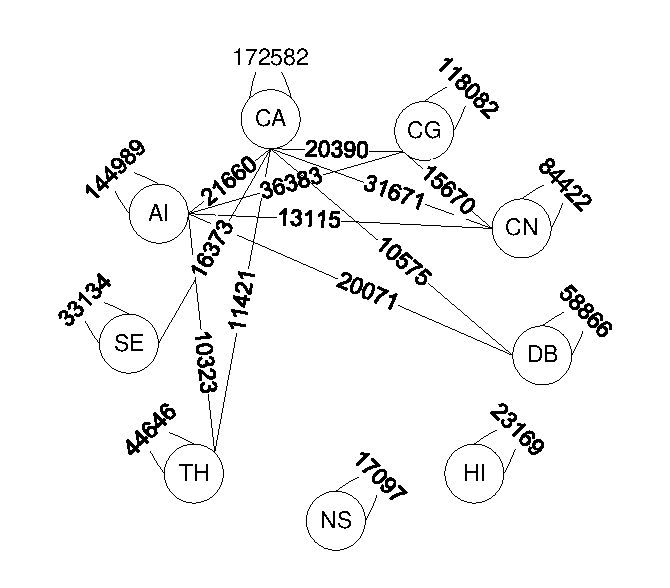
\includegraphics[width=0.23\textwidth]{fig/exp/visio_area_2001_2006.pdf}
			}
			\hspace*{-0.3cm}
			\subfigure[{\scriptsize $ Q_2 $}]{
				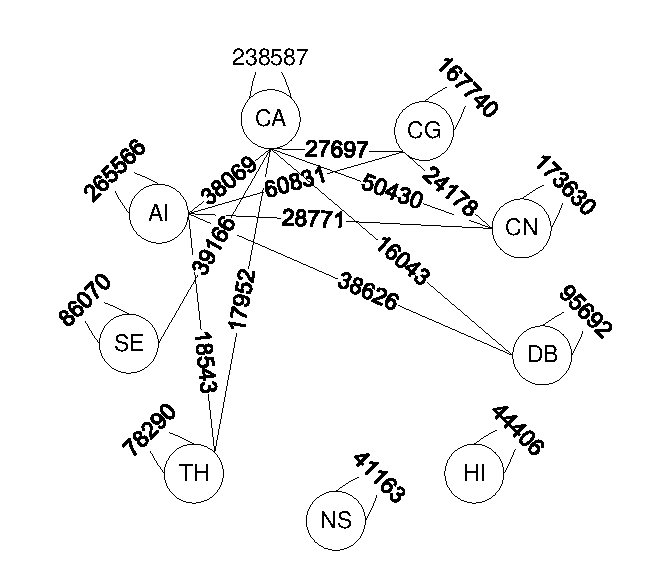
\includegraphics[width=0.23\textwidth]{fig/exp/visio_area_2006_2011.pdf}
			}
			\hspace*{-0.3cm}
			%\vspace*{-0.3cm}\\\hspace*{-0.3cm}
			\subfigure[{\scriptsize $ Q_3 $}]{
				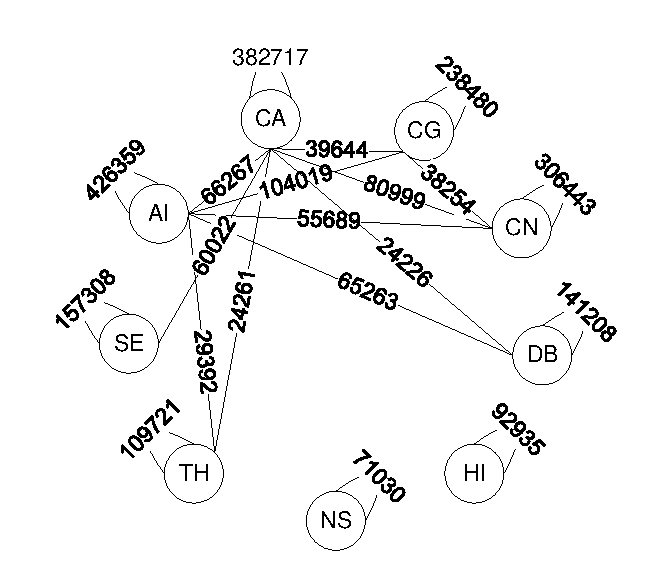
\includegraphics[width=0.23\textwidth]{fig/exp/visio_area_2011_2016.pdf}
			}
			\hspace*{-0.3cm}
			\subfigure[{\scriptsize $ Q_4 $}]{
				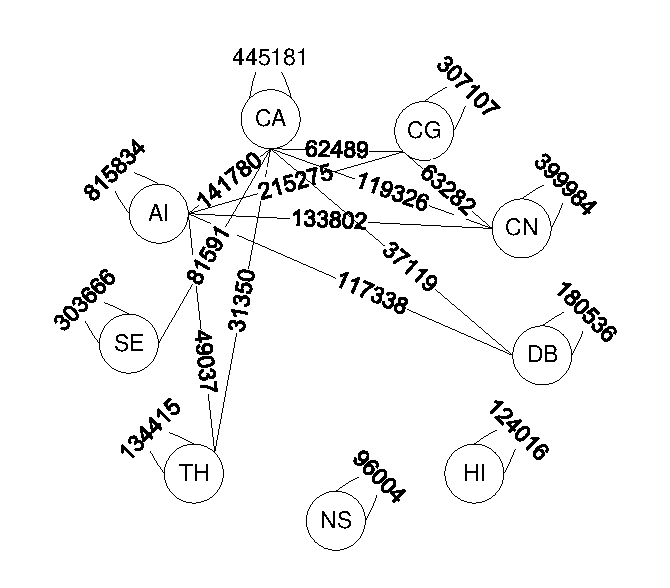
\includegraphics[width=0.23\textwidth]{fig/exp/visio_area_2016_2021.pdf}
			}
		\end{tabular}
	\end{center}
	\vspace*{-0.4cm}
	\caption{Network structures in the results of queries $ Q_1-Q_4 $}
	\vspace*{-0.4cm}
	\label{fig:dblp_area}
\end{figure*}
\comment{
The results are shown in Table~\ref{tab:vertex_table_dblp_area} and Fig.~\ref{fig:dblp_area}. The network structures of $ Q_1 $-$ Q_4 $ are shown in Fig.~\ref{fig:dblp_area}, illustrating the co-authorship patterns between authors grouped by different areas in the specified time ranges. For simplicity, in Fig.~\ref{fig:dblp_area} (a) we omit those co-authorships with COUNT($\ast$) values less than 10,000, which are also omitted in Fig.~\ref{fig:dblp_area} (b)-(d), regardless of their COUNT($\ast$) values.
}



Some interesting observations can be obtained in these results. For example, authors in each area co-author most with authors in the same area even in different time ranges. We can clearly see that in recent 20 years, the number of co-authorship between each pair of areas increases over time. We can also find that in recent 20 years researchers in \kw{AI} co-authored with researchers in \kw{CG} most. This is because there are many problems in computer graphics like automatic modeling, image processing and digital photography which can be solved by AI technologies. More interestingly, in $ [2001,2006] $, researchers in \kw{TH} co-authored most with researchers in \kw{CA}, but with the time evolves, researchers in \kw{TH} are more willing to co-author with researchers in \kw{AI}. The reason may be that theoretical research on AI becomes more and more important with the wide applications of AI in recent years. %The above findings can also be obtained from uncut results.
%[ns and cn,ca and ai;ai and cg;th and ai,ca]

In each period we can zoom into a more fine-grained view by conducting a drill-down operation. For example, for $ Q_4=((\kw{Area}),[2016,2021]) $, drill-down can be a query $ Q_4'=((\kw{Area},\kw{Productivity}),[2016,2021]) $. The network structure of $ Q_4' $ is shown in Fig.~\ref{fig:dblp_area_pro_2016_2021}.
\begin{figure}
	\begin{center}
		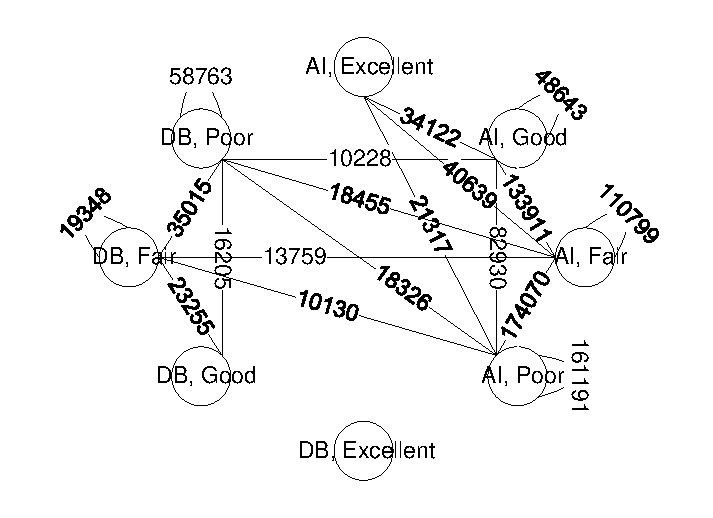
\includegraphics[width=0.8\columnwidth]{fig/exp/visio_area_pro_2016_2021.pdf}
	\end{center}
	
	\vspace*{-0.6cm}
	\caption{Network structure in the result of $ Q_4' $}
	\vspace*{-0.4cm}
	\label{fig:dblp_area_pro_2016_2021}
\end{figure}
For simplicity, we drop edges with weight less than 10,000 and we only keep vertices related to areas in $ \{\kw{AI},\kw{DB}\} $ (it can be regarded as a slice-and-dice operation). In Fig.~\ref{fig:dblp_area} (d), there are 117,338 co-authorships between researchers of \kw{AI} and \kw{DB} in $ [2016,2021] $. In fine-grained view of Fig.~\ref{fig:dblp_area_pro_2016_2021}, we can see that the most co-authorships belong to researchers of poor and fair productivity in \kw{AI} and \kw{DB}.

We then examine the effectiveness of temporal crossboid query.
\begin{figure*}[t!]
	\begin{center}
		\begin{tabular}[t]{c}\hspace*{-0.3cm}
			\subfigure[{\scriptsize $ Q_{cross1} $}]{
				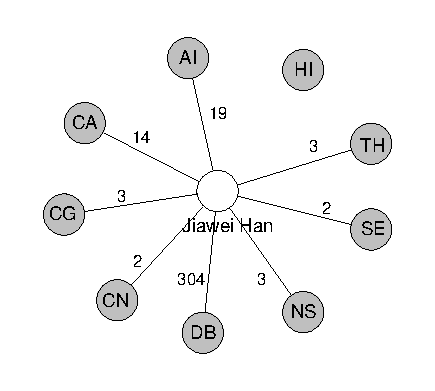
\includegraphics[width=0.25\textwidth]{fig/exp/dblp_cross_name_area_2001_2006.pdf}
			}
			\hspace*{-0.3cm}
			\subfigure[{\scriptsize $ Q_{cross2} $}]{
				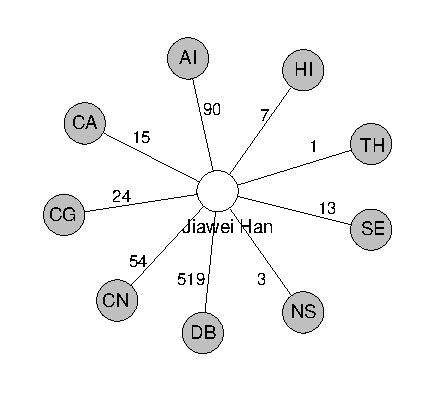
\includegraphics[width=0.25\textwidth]{fig/exp/dblp_cross_name_area_2006_2011.pdf}
			}
			\hspace*{-0.3cm}
			%\vspace*{-0.3cm}\\\hspace*{-0.3cm}
			\subfigure[{\scriptsize $ Q_{cross3} $}]{
				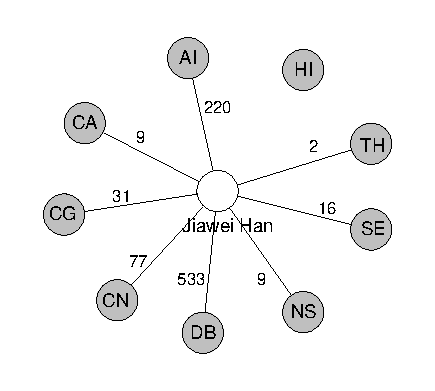
\includegraphics[width=0.25\textwidth]{fig/exp/dblp_cross_name_area_2011_2016.pdf}
			}
			\hspace*{-0.3cm}
			\subfigure[{\scriptsize $ Q_{cross4} $}]{
				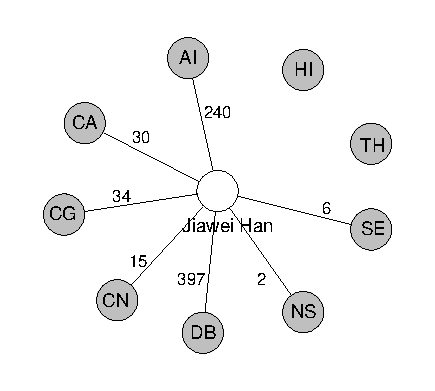
\includegraphics[width=0.25\textwidth]{fig/exp/dblp_cross_name_area_2016_2021.pdf}
			}
		\end{tabular}
	\end{center}
	\vspace*{-0.4cm}
	\caption{Network structures in the results of $ Q_{cross1}-Q_{cross4} $}
	\vspace*{-0.4cm}
	\label{fig:dblp_cross}
\end{figure*}
Fig.~\ref{fig:dblp_cross} shows the results of a series of temporal crossboid queries:
\begin{center}
	$ Q_{cross1}=((\kw{Name}),(\kw{Area}),[2001,2006]) $,\\$ Q_{cross2}=((\kw{Name}),(\kw{Area}),[2006,2011]) $,\\$ Q_{cross3}=((\kw{Name}),(\kw{Area}),[2011,2016]) $,\\$ Q_{cross4}=((\kw{Name}),(\kw{Area}),[2016,2021]) $.
\end{center}
The above queries focus on the cross interaction between \kw{Name} and \kw{Area}, i.e., the co-authorship with each area for each researcher. We further slice-and-dice the results on \kw{Name} to show the results related to ``Jiawei Han". We can find that in recent 20 years, Jiawei cooperated with researchers in \kw{DB} most. Meanwhile, in recent 10 years he has more and more cooperations with researchers in \kw{AI}, which can be ignored compared to cooperations with researchers in \kw{DB} in early 10 years.

\subsection{Efficiency Evaluation} \label{subsec:efficiency_eva}
%In this section we mainly evaluate the efficiency of temporal graph cube on \kw{IMDB}, especially the efficiency of indexes.

\stitle{Exp-1: Performance of the index-based method.} Here we aim to evaluate how much the index-based solution can accelerate the merging operation of snapshots in time ranges while processing temporal cuboid queries, compared to the baseline algorithm (Algorithm~\ref{alg:temp_cuboid_baseline}). As we analyzed before, the average acceleration ratio of the index-based solution can vary if the similarity of snapshots in temp-multi-networks changes. In this experiment, we mainly use \kw{IMDB} dataset, since vertices in \kw{IMDB} dataset have 7 dimensions and $ 2^7 $ views can be obtained. For convenience, we only materialize views in Table~\ref{tab:materialized_view}, among which we only materialize one view containing dimension \kw{Name}, because \kw{Names} of two persons are hardly the same in \kw{IMDB}, and thus \kw{Name} can be approximately regarded as a primary key and having only one view containing dimension \kw{Name} is enough.
\begin{table}[t!]%\vspace*{-0.3cm}
	\scriptsize
	%\small
	\centering
	\caption{Materialized views} \vspace*{-0.2cm} \label{tab:materialized_view}
	\begin{tabular}{c c c}
		\toprule
		\bf No. & Materialized Views & Similarity of Snapshots \cr %\hline %\hline
		\midrule
		1 & \kw{Pro} & 53.48 \cr %\hline
		\midrule
		2 & \kw{Pro}, \kw{Field} & 18.16 \cr %\hline
		\midrule
		3 & \kw{Pro}, \kw{Field}, \kw{Genre} & 6.15 \cr %\hline
		\midrule
		4 & \makecell[c]{\kw{Pro}, \kw{Field}, \kw{Genre},\\\kw{isAdult}}  & 6.07 \cr %\hline
		\midrule
		5 & \makecell[c]{\kw{Pro}, \kw{Field}, \kw{Genre},\\\kw{isAdult}, \kw{Averating}} & 4.70 \cr %\hline
		\midrule
		6 & \makecell[c]{\kw{Pro}, \kw{Field}, \kw{Genre},\\\kw{isAdult}, \kw{Averating}, \kw{Hotness}} & 3.97 \cr %\hline
		\midrule
		7 & \makecell[c]{\kw{Name}, \kw{Pro}, \kw{Field}, \kw{Genre},\\\kw{isAdult}, \kw{Averating}, \kw{Hotness}} & 1.12 \cr %\hline
		\bottomrule
	\end{tabular}
	\vspace*{-0.4cm}
\end{table}


We conduct a series of temporal cuboid queries on materialized views to examine the efficiency of the index-based method (conducting temporal cuboid queries on materialized views are all about merging snapshots in time ranges as we analyzed in Section~\ref{subsec:cuboid}). We set a series of time ranges to be specified in the queries, which are shown in Table~\ref{tab:time_ranges_set}.
\begin{table}[t!]%\vspace*{-0.3cm}
	\scriptsize
%	\small
	\centering
	\caption{Time ranges of queries} \vspace*{-0.2cm} \label{tab:time_ranges_set}
	\begin{tabular}{c c}
		\toprule
		\bf Length & Time ranges \cr %\hline %\hline
		\midrule
		4 & \makecell[c]{[1878,1880],[1891,1895],[1906,1910],\\{[1921,1925]},[1936,1940],[1951,1955],\\{[1966,1970]},[1981,1985],[1996,2000],[2011,2015]} \cr %\hline
		\midrule
		10 & \makecell[c]{[1878,1883],[1888,1898],[1903,1913],\\{[1918,1928]},[1933,1943],[1948,1958],\\{[1963,1973]},[1978,1988],[1993,2003],[2008,2018]} \cr %\hline
		\midrule
		20 & \makecell[c]{[1878,1888],[1883,1903],[1898,1918],\\{[1913,1933]},[1928,1948],[1943,1963],\\{[1958,1978]},[1973,1993],[1988,2008],[2003,2023]} \cr %\hline
		\midrule
		50 & \makecell[c]{[1878,1903],[1878,1918],[1883,1933],\\{[1898,1948]},[1913,1963],[1928,1978],\\{[1943,1993]},[1958,2008],[1973,2023],[1988,2028]} \cr %\hline
		\midrule
		100 & \makecell[c]{[1878,1928],[1878,1943],[1878,1958],\\{[1878,1973]},[1888,1988],[1903,2003],\\{[1918,2018]},[1933,2028],[1948,2028],[1963,2028]} \cr %\hline
		\bottomrule
	\end{tabular}
	\vspace*{-0.4cm}
\end{table}
The earliest and the latest timestamps in \imdb are 1878 and 2028 respectively. We set 5 groups of time ranges of different length: 4, 10, 20, 50, 100. For each length, we set 10 ranges which are evenly distributed in $ [1878,2028] $ as shown in Table~\ref{tab:time_ranges_set}. Ranges at two ends in each length group may be truncated since we try to keep each time range in $ [1878,2028] $. Specifically, we set a series of queries $ QS_1,QS_2,...,QS_7 $, where $ QS_i $ is a set of queries specifying the No.$ i $ materialized view in Table~\ref{tab:materialized_view} and covering all time ranges of all lengths in Table~\ref{tab:time_ranges_set}, i.e., $ QS_1=\{((Pro),[1878,1880]),...,((Pro),[2011,2015]),\\((Pro),[1878,1883]),...,((Pro),[2008,2018]),...,\\((Pro),[1878,1928]),...,((Pro),[1963,2028])\} $.

\comment{
\begin{table}[t!]%\vspace*{-0.3cm}
	\scriptsize
	%\small
	\centering
	\caption{Performance of the index-based solution} \vspace*{-0.2cm} \label{tab:effi_prearray}
	\begin{tabular}{c c c c c| c c c}
		\toprule
		\makecell[c]{Views\\No.}& $ s $ & \makecell[c]{baseline\\(ms)} &\makecell[c]{STree\\(ms)}&\makecell[c]{acce-ratio\\(ave)} & \makecell[c]{Original\\view size} &  \makecell[c]{STree\\size}&\makecell[c]{STree\\ratio}\cr %\hline %\hline
		\midrule
		1&53.48&16,960 &3,960 &3.45 &41,448 &93,975 &2.27 \cr
		\midrule
		2&18.16&172,614 &57,637 &2.32 &396,755 &1,077,456 &2.72\cr
		\midrule
		3&6.15&279,684 &144,849 &1.59&3,738,125 &13,788,570 &3.69\cr
		\midrule
		4&6.07&285,623 &147,565 &1.59&3,758,885 &13,918,066 &3.70 \cr
		\midrule
		5&4.70&515,607 &293,546 &1.50&5,467,826 &22,063,352 &4.04\cr
		\midrule
		6&3.97&896,386 &550,376 &1.40&8,304,421 &35,837,987 &4.32\cr
		\midrule
		7&1.12&6,719,417 &6,366,660 &1.05&37,096,632 &285,623,583 &7.70\cr
		\bottomrule
	\end{tabular}
	\vspace*{-0.4cm}
\end{table}


\begin{table}[t!]%\vspace*{-0.3cm}
	\scriptsize
	%\small
	\centering
	\caption{Performance of the index-based solution} \vspace*{-0.2cm} \label{tab:effi_prearray}
	\begin{tabular}{c c c c c| c c c}
		\toprule
		\makecell[c]{Views\\No.}& $ s $ & \makecell[c]{baseline\\(ms)} &\makecell[c]{STree\\(ms)}&\makecell[c]{acce-ratio\\(ave)} & \makecell[c]{Original\\view size} &  \makecell[c]{STree\\size}&\makecell[c]{STree\\ratio}\cr %\hline %\hline
		\midrule
		1&53.48&16,960 &3,960 &3.45 &41KB &94KB &2.27 \cr
		\midrule
		2&18.16&172,614 &57,637 &2.32 &397KB &1.1MB &2.72\cr
		\midrule
		3&6.15&279,684 &144,849 &1.59&3.7MB &13.8MB &3.69\cr
		\midrule
		4&6.07&285,623 &147,565 &1.59&3.8MB &13.9MB &3.70 \cr
		\midrule
		5&4.70&515,607 &293,546 &1.50&5.4MB &22.1MB &4.04\cr
		\midrule
		6&3.97&896,386 &550,376 &1.40&8.3MB &35.8MB &4.32\cr
		\midrule
		7&1.12&6,719,417 &6,366,660 &1.05&37.1MB &285.6MB &7.70\cr
		\bottomrule
	\end{tabular}
	\vspace*{-0.4cm}
\end{table}
}

\begin{table}[t!]%\vspace*{-0.3cm}
	\scriptsize
	%\small
	\centering
	\caption{Performance of the index-based solution (K=1,000, M=1,000,000)} \vspace*{-0.2cm} \label{tab:effi_index}
	\begin{tabular}{c c c c c c c c}
		\toprule
		\makecell[c]{View\\No.}& $ s $ & \makecell[c]{Baseline\\(sec.)} &\makecell[c]{STree\\(sec.)}&\makecell[c]{acce-ratio\\(ave)} & \makecell[c]{View\\ size} &  \makecell[c]{STree\\size}&\makecell[c]{Space\\ratio}\cr %\hline %\hline
		\midrule
		1&53.48&17 &4 &4.25 &41K &94K &2.29 \cr
		\midrule
		2&18.16&173 &58 &2.98 &397K &1.1M &2.77\cr
		\midrule
		3&6.15&280 &145 &1.93&3.7M &13.8M &3.72\cr
		\midrule
		4&6.07&286 &148 &1.93&3.7M &13.9M &3.76 \cr
		\midrule
		5&4.70&516 &294 &1.76&5.4M &22.1M &4.09\cr
		\midrule
		6&3.97&896 &550 &1.63&8.3M &35.8M &4.31\cr
		\midrule
		7&1.12&6,719 &6,367 &1.06&37.1M &285.6M &7.70\cr
		\bottomrule
	\end{tabular}
	\vspace*{-0.4cm}
\end{table}

We set $ f_e= $ MAX($\ast$) and use the queries in $ QS_1,\cdots,QS_7 $ to test the efficiency of our index-based algorithm. The results are shown in Table~\ref{tab:effi_index}. Similar results can also be observed for the other aggregation functions ($ f_e= $ COUNT($\ast$), $ f_e= $ SUM($\ast$), and $ f_e= $ MIN($\ast$)). In Table~\ref{tab:effi_index}, \kw{View No.} denotes the No. of materialized views in Table~\ref{tab:materialized_view}, and $ s $ is the similarity of snapshots. The third and the fourth columns are time used to process all the queries on each materialized view using the baseline method and the index-based algorithm respectively. For example, in the first line, processing all queries in $ QS_1 $ takes $ 17s $ using the baseline method, but consumes $ 4s $ using the segment-tree index based algorithm. The \kw{acce-ratio(ave)} is the average acceleration ratio of the index-based algorithm on each query, compared to the baseline algorithm. In most cases, the index-based algorithm can accelerate merging snapshots in time ranges in conducting queries. However, the effect of acceleration varies with $ s $. In the No.1 view, where $s$ is the largest, we can see that the index-based solution achieves the best average acceleration ratio. We can observe that the average acceleration ratio of the index-based solution drops if $ s $ drops in general, which confirms our analysis in Section~\ref{sec:effec_of_indexes}. 

Table~\ref{tab:effi_index} also shows the space usage of the index-based solution (6th-8th columns). As can be seen, the size of the segment-tree based index is only several times larger than the original size of the views. For example, in the first line, the original view size is 41K, while our index-based solution takes only 94K space, with 2.27\kw{x} more space usage. Also, we can see that with $s$ increasing, the space usage of the index-based solution decreases. These results demonstrate that our segment-tree based index structure is very space-efficient when $s$ is relatively large. However, when $s$ is small, e.g., near to 1, the space overhead of our index-based solution is high. Moreover, when $s$ is near to 1, the average acceleration ratio is also near to 1 (i.e., the index-based solution is only slightly better than the baseline method). These results indicate that when $s$ is very small, there is no need to build an index.


\stitle{Exp-2: Updating performance of the index-based solution.} Here we evaluate the updating performance of our index-based solution. We divide all temporal edges in a materialized view into 10 batches equally according to the order of timestamps, e.g., the first batch of temporal edges are edges with the smallest timestamps, and they are added into the index one by one following the order of timestamps. When edges in a single batch are added into the index, we record both the time and space consumption of adding edges in the batch. The results are shown in Fig.~\ref{fig:index_update}. From Fig.~\ref{fig:index_update}(a), we can see that with the number of batch increasing, the time consumption of the index-updating algorithm increases. These results are consistent with our analysis in Section~\ref{subsec:segment_tree}. Moreover, we can observe that for a large $s$, the time cost of our index-updating algorithm is low, while for a small $s$, the cost is often high. The reason could be that updating STree involves copying snapshot, i.e., snapshot in root, which maintains all snapshots in snapshot array, and thus gets larger if $ s $ gets smaller. As shown in Fig.~\ref{fig:index_update}(b), the space consumption of the index-updating algorithm is linear with respect to the number of batches, indicating that our algorithm is space-efficient. Likewise, we can observe that the algorithm takes more space for a smaller $s$. These results further confirm our analysis in Section~\ref{subsec:segment_tree}.


\begin{figure}[t!]
	\begin{center}
		\begin{tabular}[t]{c}\hspace*{-0.3cm}
		%	\subfigure[{\scriptsize Prefix Array}]{
%				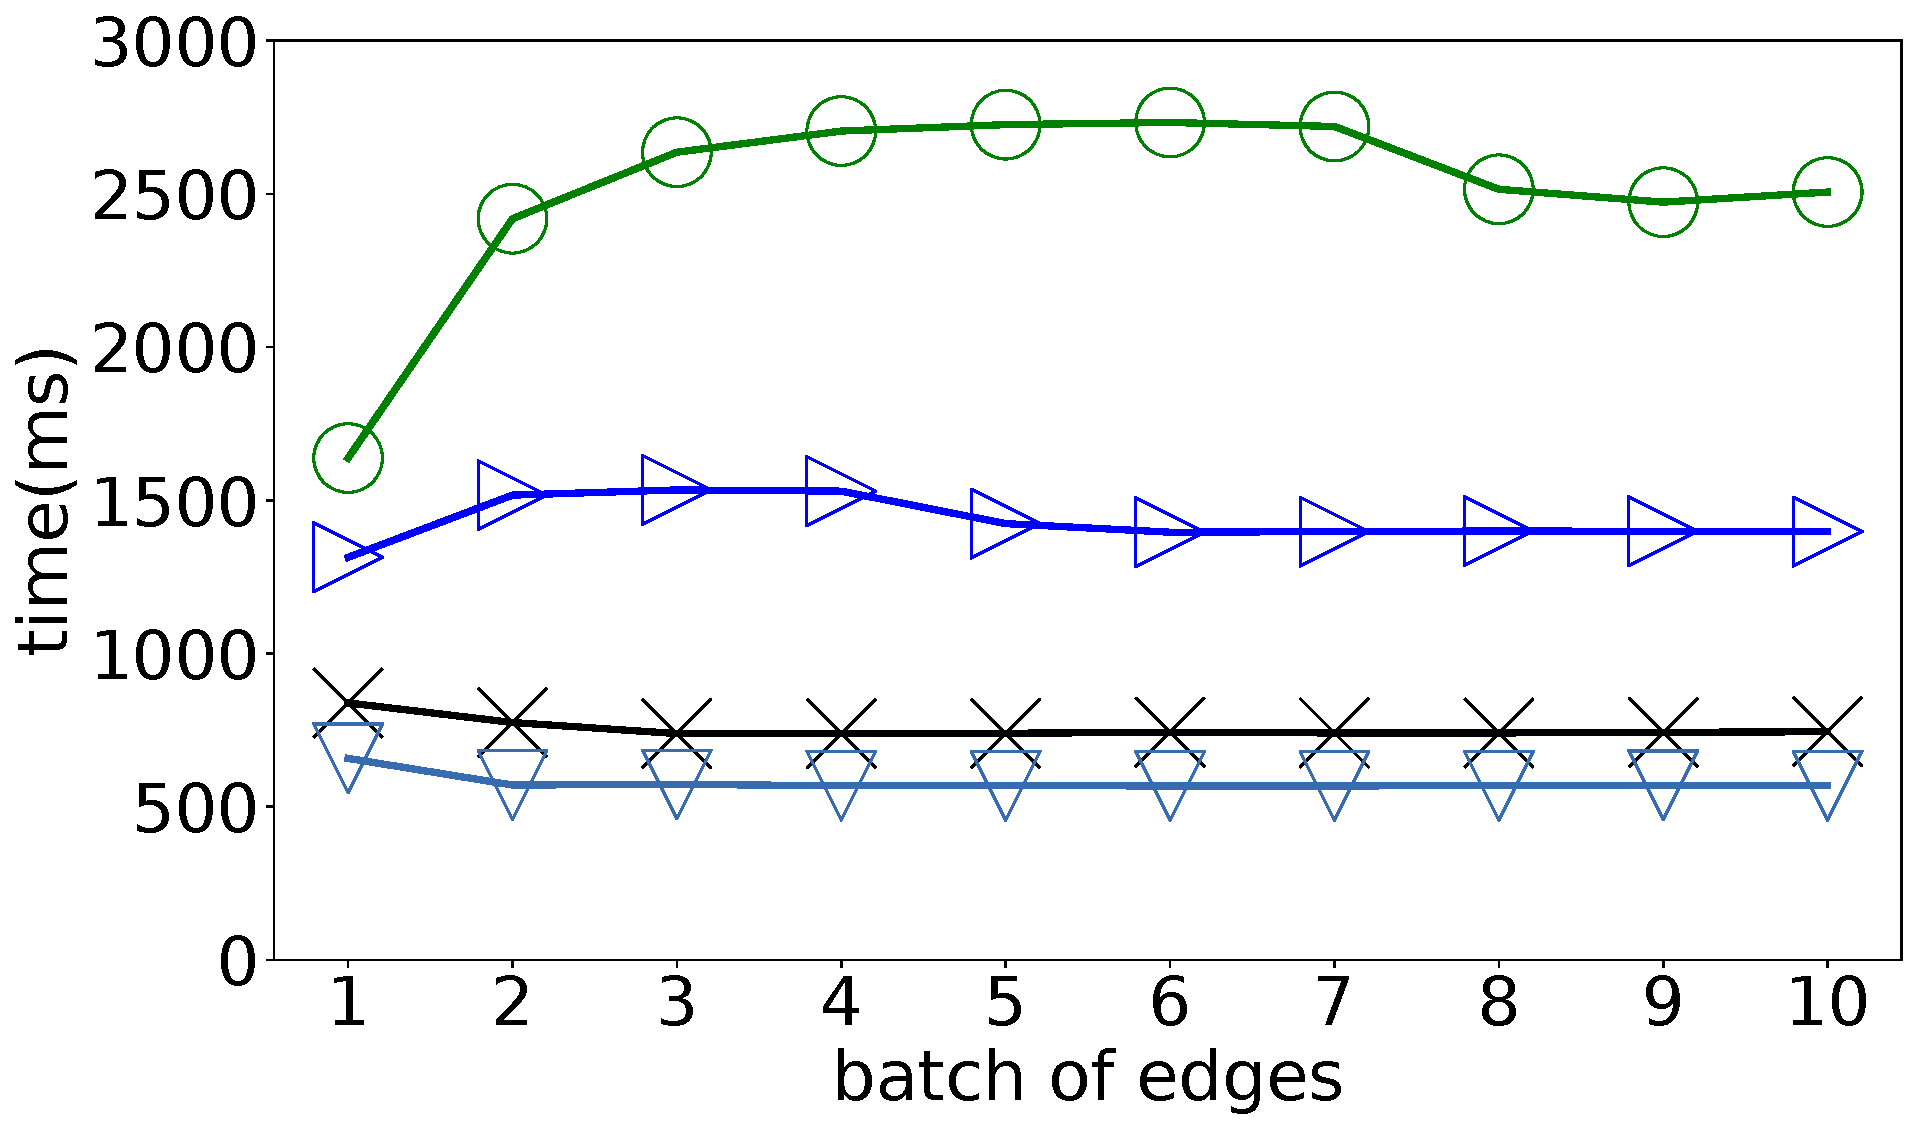
\includegraphics[width=0.25\textwidth]{fig/exp/index_update/index_update_single_a.pdf}
%			}
%			\hspace*{-0.3cm}
%			\subfigure[{\scriptsize STable}]{
%				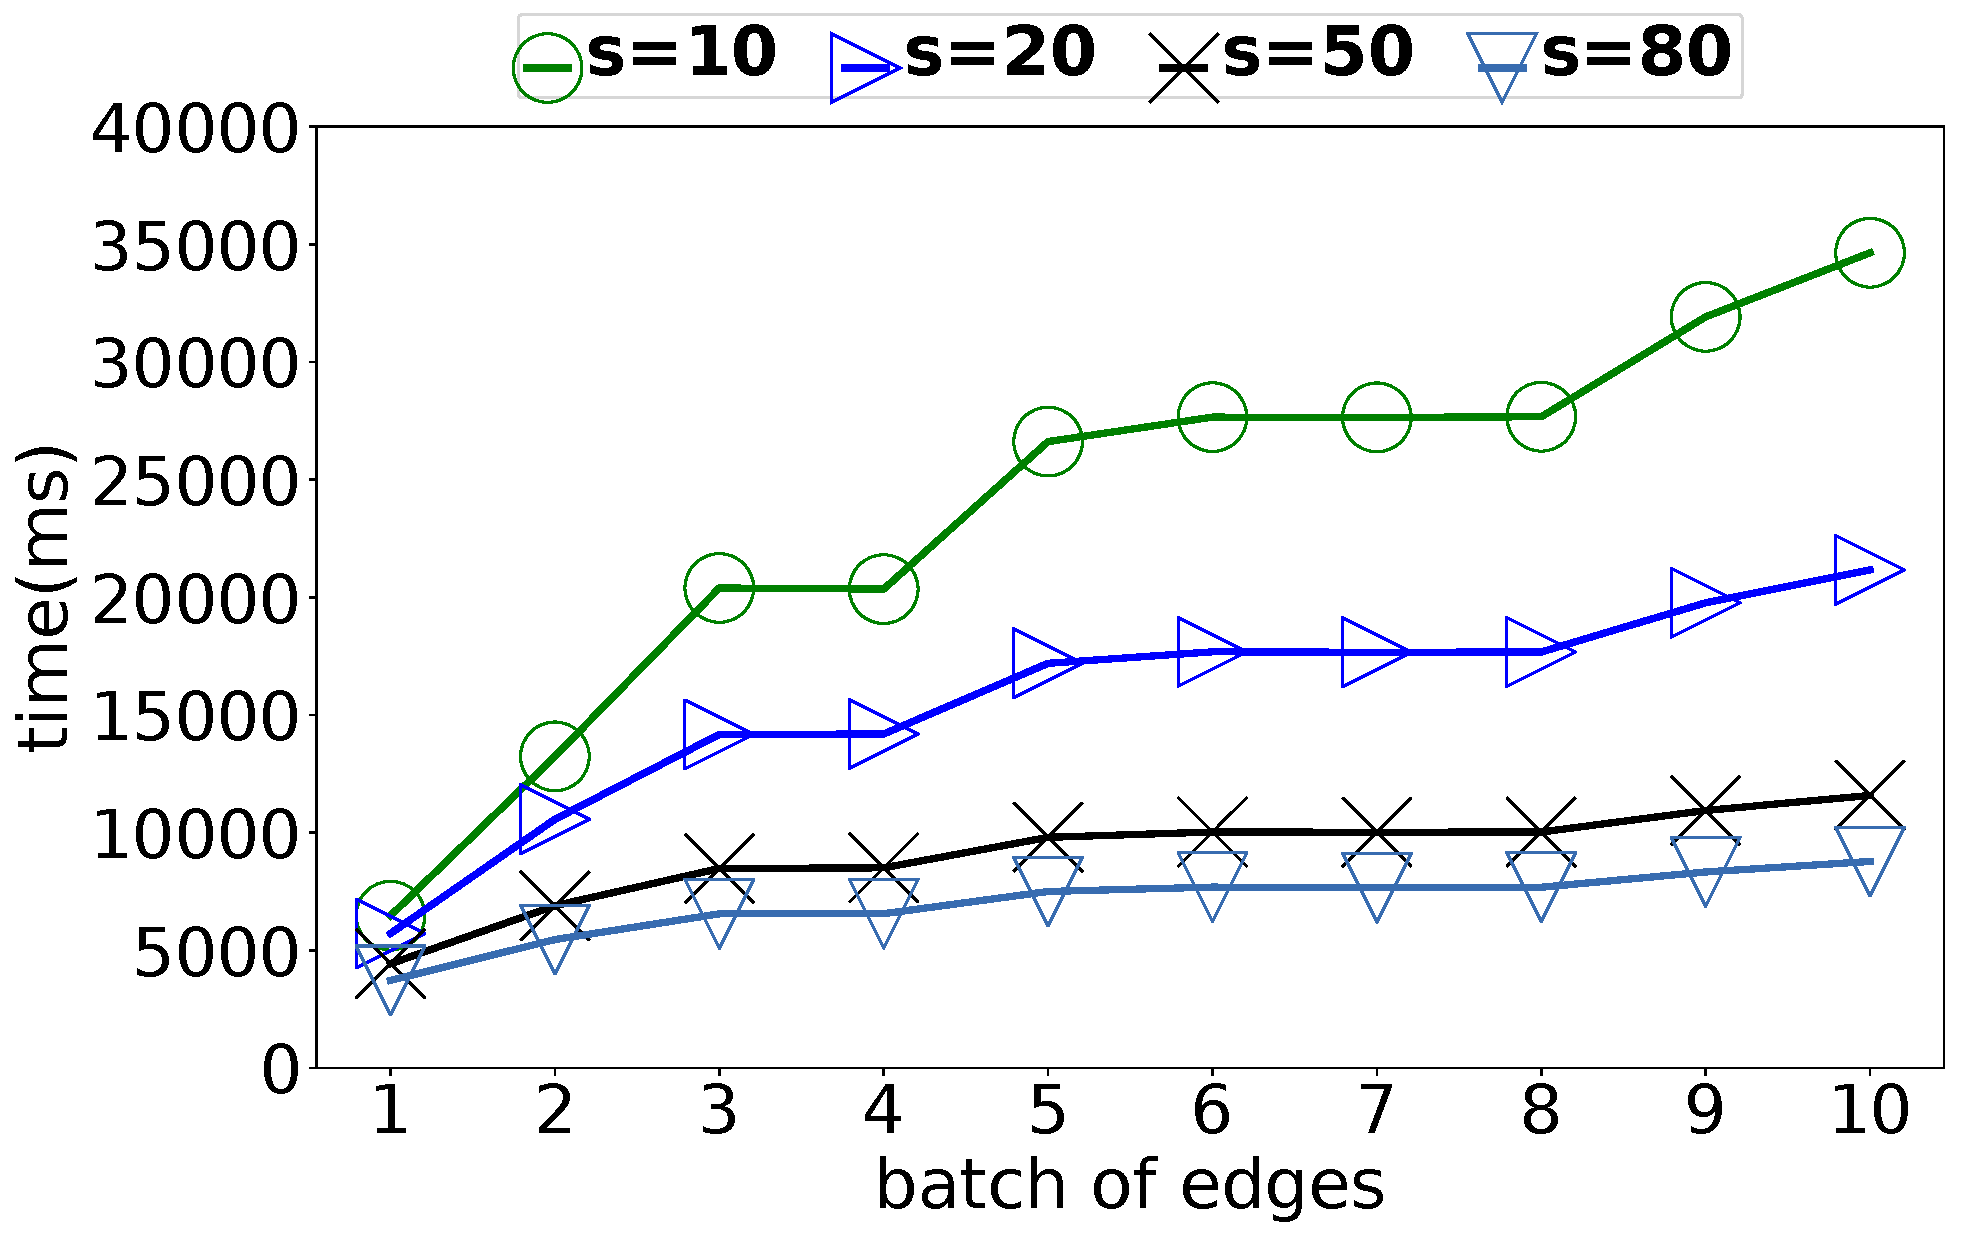
\includegraphics[width=0.25\textwidth]{fig/exp/index_update/index_update_single_b.pdf}
%			}
%			\hspace*{-0.3cm}
%			%\vspace*{-0.3cm}\\\hspace*{-0.3cm}
			\subfigure[{\scriptsize Time consumption}]{
				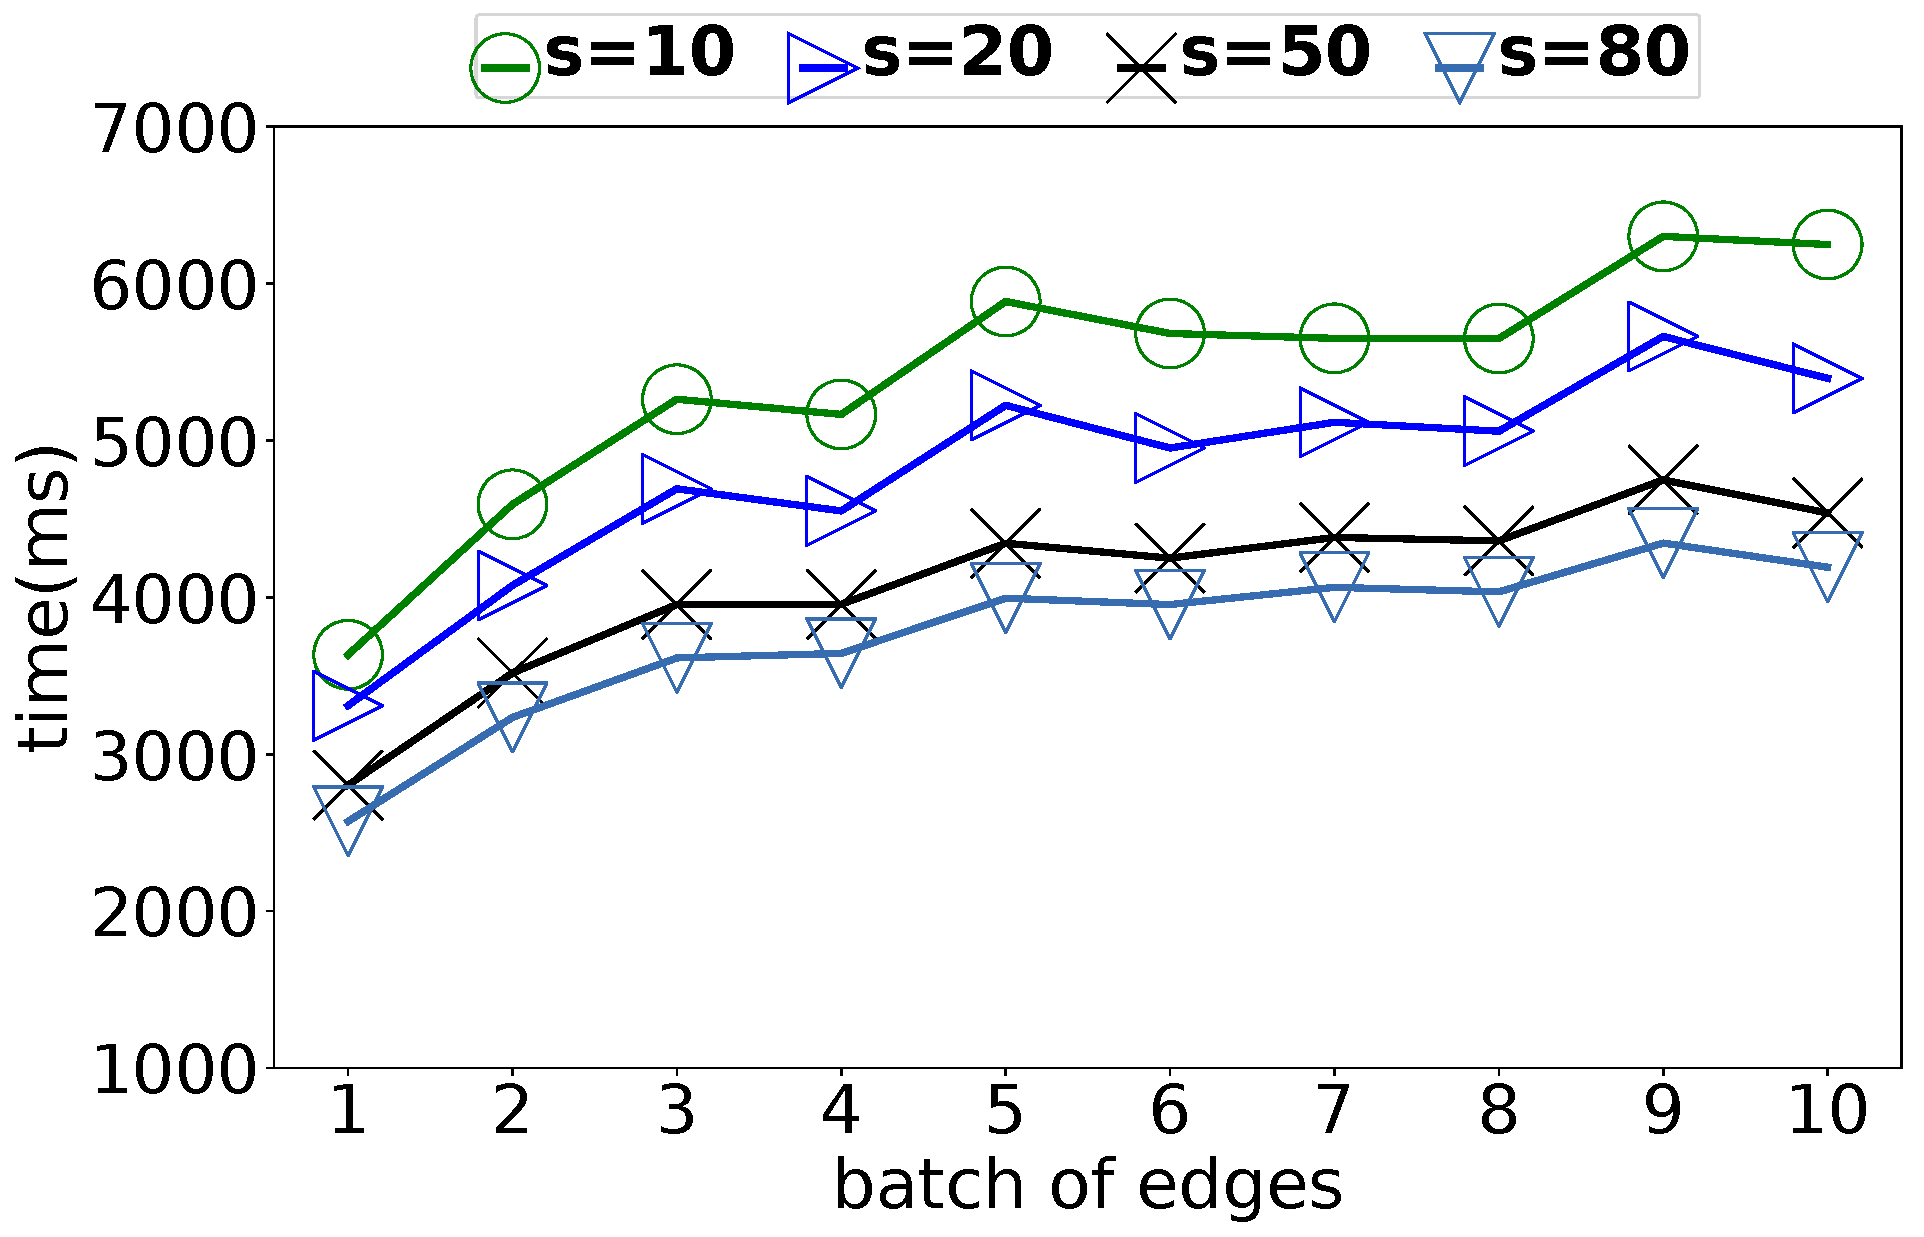
\includegraphics[width=0.23\textwidth]{fig/exp/index_update/index_update_single_c.pdf}
			}
	%		\\
%			\hspace*{-0.3cm}
%			\subfigure[{\scriptsize Prefix Array}]{
%				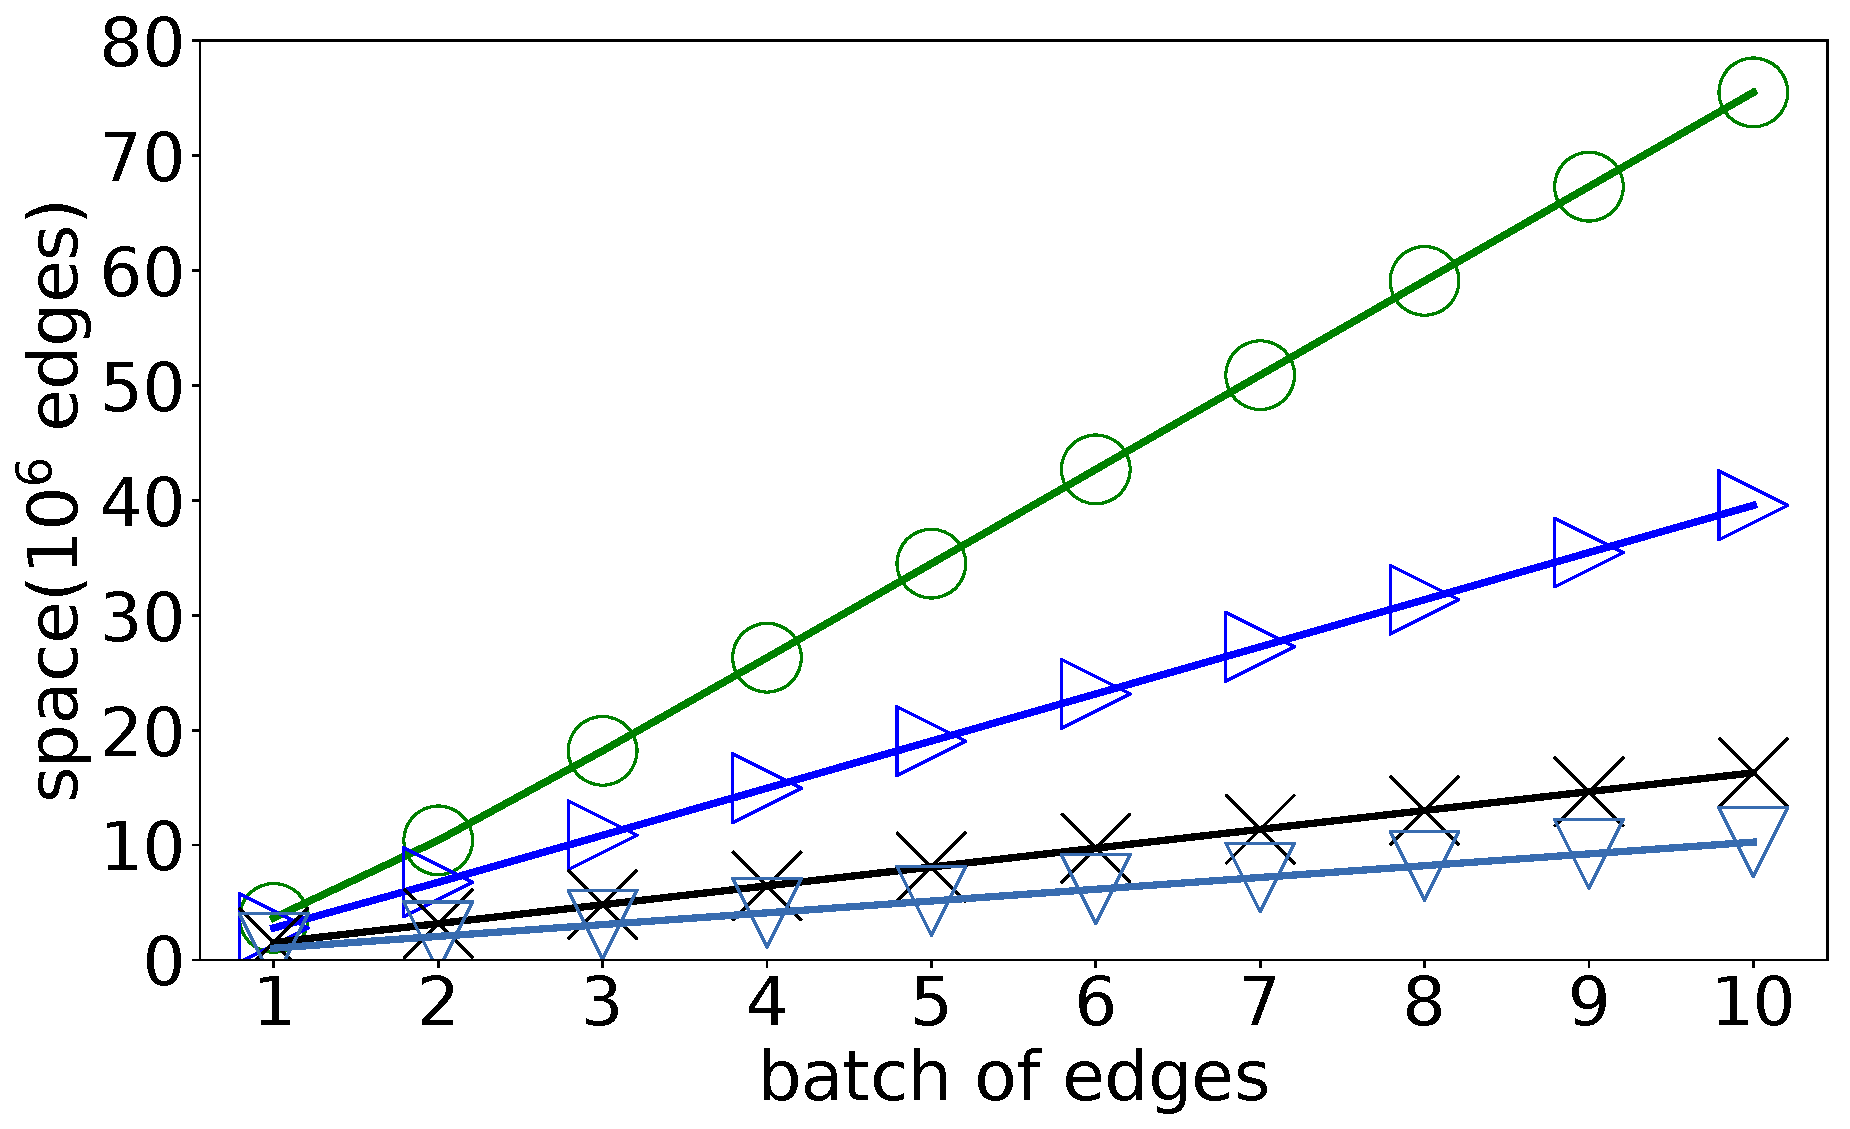
\includegraphics[width=0.25\textwidth]{fig/exp/index_update/index_update_single_d.pdf}
%			}
%			\hspace*{-0.3cm}
%			\subfigure[{\scriptsize STable}]{
%				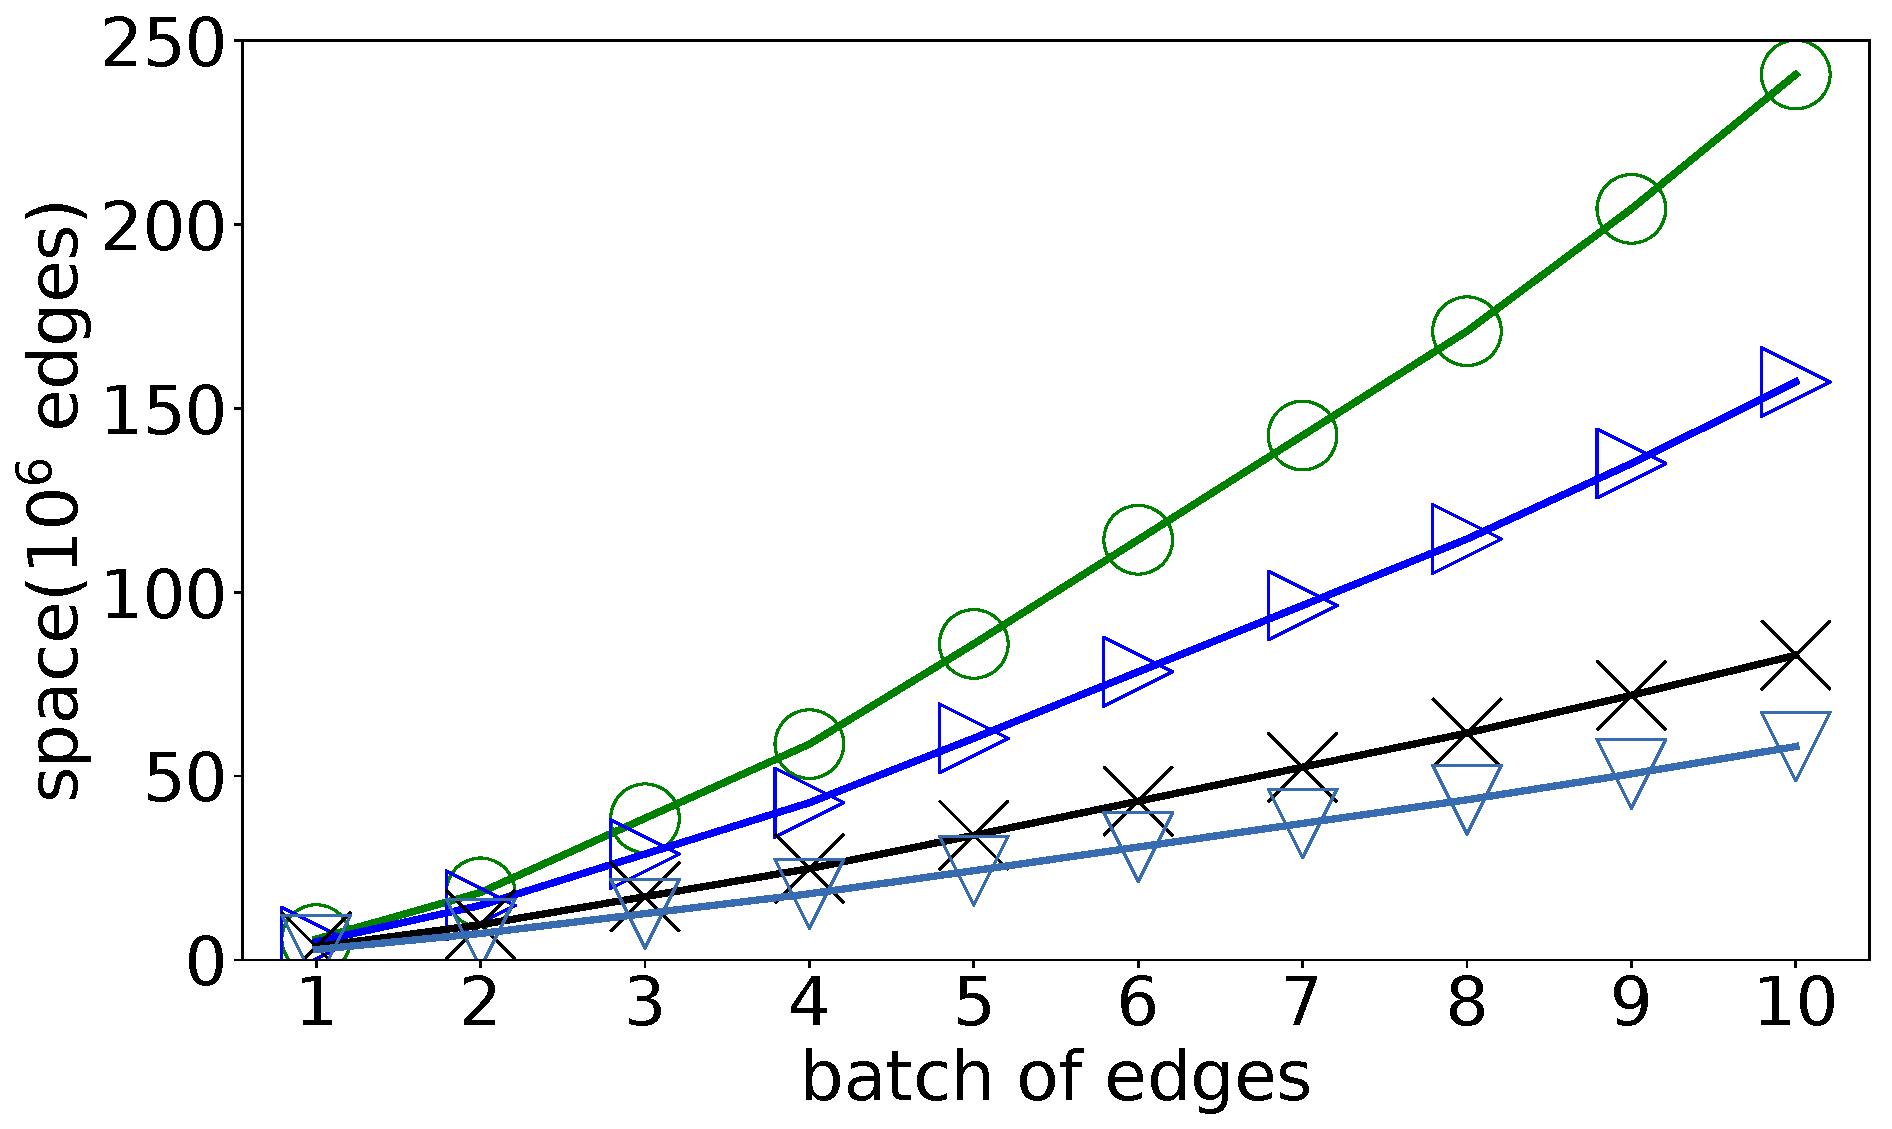
\includegraphics[width=0.25\textwidth]{fig/exp/index_update/index_update_single_e.pdf}
%			}
			\hspace*{-0.3cm}
			\subfigure[{\scriptsize Space usage}]{
				\includegraphics[width=0.23\textwidth]{fig/exp/index_update/index_update_single_f.pdf}
			}
		\end{tabular}
	\end{center}
	\vspace*{-0.5cm}
	\caption{The updating performance of the index-based solution}
	\vspace*{-0.4cm}
	\label{fig:index_update}
\end{figure}




\section{Related Work} \label{sec:related_work}
Our work extends data warehouse and OLAP techniques to temporal multidimensional networks. There are many works applying data warehouse and OLAP to other data types, such as stream data \cite{han2005stream}, spatio-temporal data \cite{gomez2009survey}, sequence data \cite{lo2008olap,liu2011cube}, and text data \cite{lin2008text}. Except the traditional relational data, Dehdouh et al. \cite{dehdouh2014columnar} tried to compute data cubes from column-oriented NoSQL data. As for graph data, except \cite{zhao2011graph}, some other works focus on heterogeneous networks \cite{yin2012hmgraph,wang2015tsmh}. \revision{\cite{wang2014pagrol,chen2020high} improve efficiency of graph OLAP query by parallelization and distribution}. However, none of them focus on temporal multidimensional networks.

Our work is also related to graph summarization and analysis. For static graphs, there are some representative works, including graph compression with MDL (Minimum Description Length) principle \cite{navlakha2008graph}, attributed graph compression \cite{wu2014graph} and graph clustering based on vertices partitioning \cite{zhou2009graph}. Recently, there exist several studies on static graph summarization, such as summarizing directed acyclic graph (DAG) \cite{zhu2020top}, summarizing multi-relation graph \cite{ke2022multi} where multiple edges of different types may exist between any pair of vertices, and DPGS model \cite{zhou2021dpgs}, which can preserve properties like graph spectrum and the authorities and hubnesses of vertices while reconstructing graph. \revision{However, all of them ignore the temporal information of big graph data}. For temporal graph and dynamic graph, TimeCrunch \cite{shah2015timecrunch} summarizes a large dynamic graph with a set of important temporal structures using MDL, such as ranged full clique, periodic bipartite core, oneshot star, etc. \revision{Some works (\cite{mudannayake2021kmatrix,tang2016graph,ma2021parameter,ashrafi2021gs4,gou2019fast,chen2022scube}) summarize graph stream into one sketche. \cite{fernandes2018dynamic,tsalouchidou2018scalable} use a sliding window of fixed length to only summarize the latest snapshots, and \cite{ko2020incremental} only summarize the current snapshot of a graph stream incrementally and losslessly}. However, in this paper, we can specify arbitrary time window to query summarized result in real time. \revision{Chen et al. \cite{chen2022horae} also studies summarizing snapshots in arbitrary time window, but they ignored the attributes of vertices and different views determined by combinations of those attributes}. We summarize graphs based on selected attributes of vertices, \revision{so we can get summarized information between vertices in different resolutions.}

\section{Conclusion} \label{sec:conclusion}
In this paper, we extend data warehouse and OLAP technology to temporal multidimensional networks by proposing a new data warehouse model \kw{Temporal\enspace Graph\enspace Cube}, which provides knowledge workers with tools to analyze temporal multidimensional networks. We first extend the basic concepts in static graph cube and introduce two new queries, \kw{temporal\enspace cuboid} and \kw{temporal\enspace crossboid}, allowing \kw{Temporal\enspace Graph\enspace Cube} to support OLAP queries on temporal multidimensional networks. Then, we propose a segment-tree based index method to accelerate the OLAP queries. We also present a new metric to measure the efficiency of the index. We conduct extensive experiments on two large real-world datasets, and the results demonstrate the effectiveness and efficiency of the proposed solutions.

%We point out that some classical methods are no longer applicable in the implementation of \kw{Temporal\enspace Graph\enspace Cube}.

%Our experimental results show the effectiveness of \kw{Temporal\enspace Graph\enspace Cube} and corroborate our inferences about the relationship between the efficiency of indexes and the metric. With the support of the implementation strategy for \kw{Temporal\enspace Graph\enspace Cube}, the indexes are able to achieve an acceleration effect. Moreover, the best time and space balance, as well as the best scalability, is achieved by segment tree among the three indexes.


% if have a single appendix:
%\appendix[Proof of the Zonklar Equations]
% or
%\appendix  % for no appendix heading
% do not use \section anymore after \appendix, only \section*
% is possibly needed

% use appendices with more than one appendix
% then use \section to start each appendix
% you must declare a \section before using any
% \subsection or using \label (\appendices by itself
% starts a section numbered zero.)
%

\comment{

% use section* for acknowledgment
\ifCLASSOPTIONcompsoc
% The Computer Society usually uses the plural form
\section*{Acknowledgments}
\else
% regular IEEE prefers the singular form
\section*{Acknowledgment}
\fi
This work was partially supported by (i) National Key Research and Development Program of China 2020AAA0108503, (ii) NSFC Grants 62072034 and 61772346, and (iii) CCF-Baidu Open Fund;
%(ii) NSFC Grants 61772346, 61732003, U1809206, 61772091, 61802035;
%(iii) Beijing Institute of Technology Research Fund Program for Young Scholars;
%(iv) Research Grants Council of the Hong Kong SAR, China No. 14221716 and 14203618;
%(v) ARC Discovery Project Grant DP160101513;
%and (vi) MOE, Singapore under grant MOE2015-T2-2-069 and NUS, Singapore under an SUG.


% Can use something like this to put references on a page
% by themselves when using endfloat and the captionsoff option.
\ifCLASSOPTIONcaptionsoff
\newpage
\fi

}

% trigger a \newpage just before the given reference
% number - used to balance the columns on the last page
% adjust value as needed - may need to be readjusted if
% the document is modified later
%\IEEEtriggeratref{8}
% The "triggered" command can be changed if desired:
%\IEEEtriggercmd{\enlargethispage{-5in}}

% references section

% can use a bibliography generated by BibTeX as a .bbl file
% BibTeX documentation can be easily obtained at:
% http://mirror.ctan.org/biblio/bibtex/contrib/doc/
% The IEEEtran BibTeX style support page is at:
% http://www.michaelshell.org/tex/ieeetran/bibtex/
%\bibliographystyle{IEEEtran}
% argument is your BibTeX string definitions and bibliography database(s)
%\bibliography{IEEEabrv,../bib/paper}
%
% <OR> manually copy in the resultant .bbl file
% set second argument of \begin to the number of references
% (used to reserve space for the reference number labels box)

%\balance
\bibliographystyle{IEEEtran}
\bibliography{IEEEabrv,temporal_graph_cube}

%\begin{thebibliography}{1}
%
%\bibitem{IEEEhowto:kopka}
%H.~Kopka and P.~W. Daly, \emph{A Guide to \LaTeX}, 3rd~ed.\hskip 1em plus
%  0.5em minus 0.4em\relax Harlow, England: Addison-Wesley, 1999.
%
%\end{thebibliography}

% biography section
%
% If you have an EPS/PDF photo (graphicx package needed) extra braces are
% needed around the contents of the optional argument to biography to prevent
% the LaTeX parser from getting confused when it sees the complicated
% \includegraphics command within an optional argument. (You could create
% your own custom macro containing the \includegraphics command to make things
% simpler here.)
%\begin{IEEEbiography}[{\includegraphics[width=1in,height=1.25in,clip,keepaspectratio]{mshell}}]{Michael Shell}
% or if you just want to reserve a space for a photo:
\vspace*{-20mm}




% if you will not have a photo at all:
%\begin{IEEEbiographynophoto}{Rong-Hua Li}
%Biography text here.
%\end{IEEEbiographynophoto}

% insert where needed to balance the two columns on the last page with
% biographies
%\newpage

%\begin{IEEEbiographynophoto}{Jane Doe}
%Biography text here.
%\end{IEEEbiographynophoto}

% You can push biographies down or up by placing
% a \vfill before or after them. The appropriate
% use of \vfill depends on what kind of text is
% on the last page and whether or not the columns
% are being equalized.

%\vfill

% Can be used to pull up biographies so that the bottom of the last one
% is flush with the other column.
%\enlargethispage{-5in}



% that's all folks

\begin{IEEEbiography}[{\includegraphics[width=1in,height=1.25in,clip,keepaspectratio]{biophoto/grwang.jpg}}]{Guoren Wang}
	received the BS, MS, and PhD degrees from the Department of Computer Science, Northeastern University, China, in 1988, 1991, and
1996, respectively. Currently, he is a professor with the Beijing Institute of Technology (BIT), Beijing, China. His research interests include graph data management, graph mining, and graph computational systems.
\end{IEEEbiography}
\vspace{-10ex}
\begin{IEEEbiography}[{\includegraphics[width=1in,height=1.25in,clip,keepaspectratio]{biophoto/yuez.jpg}}]{Yue Zeng}
	is currently a master student at Beijing Institute of Technology (BIT), Beijing, China. His research interests include graph data management and social network analysis.
\end{IEEEbiography}
\vspace{-10ex}
\begin{IEEEbiography}[{\includegraphics[width=1in,height=1.25in,clip,keepaspectratio]{biophoto/RonghuaLi}}]{Rong-Hua Li}
	received the PhD degree from the Chinese University of Hong Kong, in 2013. He is currently a professor with the Beijing Institute of Technology (BIT), Beijing, China. His research interests include graph data management and mining, social network analysis, graph computational systems, and graph-based machine learning.
\end{IEEEbiography}
\vspace{-10ex}
\begin{IEEEbiography}[{\includegraphics[width=1in,height=1.30in,clip,keepaspectratio]{biophoto/hcqin}}]{Hongchao Qin}
is currently a Postdoc at Beijing Institute of Technology, China. He received the B.S. degree in mathematics, M.E. degree and Ph.D. degree in computer science from Northeastern University, China in 2013, 2015 and 2020, respectively. His current research interests include social network analysis and data-driven graph mining.
\end{IEEEbiography}
\vspace{-10ex}
\begin{IEEEbiography}[{\includegraphics[width=1in,height=1.30in,clip,keepaspectratio]{biophoto/xhshi.jpg}}]{Xuanhua Shi}
received his Ph.D. degree in Computer Engineering from HUST (China) in 2005. He is a professor in Service Computing Technology and System Lab and Cluster and Grid
Computing Lab, HUST (China). His current research interests focus on the scalability, resilience and autonomy of large-scale distributed systems, such as peta-scale systems, and data centers.
\end{IEEEbiography}
\vspace{-10ex}
\begin{IEEEbiography}[{\includegraphics[width=1in,height=1.30in,clip,keepaspectratio]{biophoto/ybxia.jpg}}]{Yubin Xia}
received the deploma degree in software school, Fudan University, Shanghai, China, in 2004, and the Ph.D. degree in computer science and technology from Peking University, Beijing, China, in 2010. He is now an associate professor in Shanghai Jiao Tong University since September 2012. His research interests include computer architecture, operating system, and security.
\end{IEEEbiography}
\vspace{-10ex}
\begin{IEEEbiography}[{\includegraphics[width=1in,height=1.30in,clip,keepaspectratio]{biophoto/xqshang.jpg}}]{Xuequn Shang} 
received her Ph.D. in computer science from University of Magdeburg, Germany, in 2005. She is currently a professor in School of Computer Science, Northwestern Polytechnical University, China. Her research interests include data mining, bioinformatics and machine learning.
\end{IEEEbiography}
\vspace{-10ex}
\begin{IEEEbiography}[{\includegraphics[width=1in,height=1.30in,clip,keepaspectratio]{biophoto/lhong}}]{Liang Hong}
received his BS degree and Ph.D. degree in Computer Science at Huazhong University of Science and Technology (HUST) in 2003 and 2009, respectively. Now, he is an associate professor
in School of Information Management of Wuhan University. His research interests include graph database, spatio-temporal data management and social networks.
\end{IEEEbiography}

%\begin{IEEEbiography}[{\includegraphics[width=1in,height=1.25in,clip,keepaspectratio]{biophoto/wanggr}}]{Guoren Wang}
%	received the BS, MS, and PhD degrees from the Department of Computer Science, Northeastern University, China, in 1988, 1991, and
%1996, respectively. Currently, he is a professor with the Beijing Institute of Technology (BIT), Beijing, China. His research interests include graph data management, graph mining, and graph computational systems. 
%\end{IEEEbiography}
%
%\begin{IEEEbiography}[{\includegraphics[width=1in,height=1.25in,clip,keepaspectratio]{biophoto/zengyue}}]{Yue Zeng}
%	is currently a master student at Beijing Institute of Technology (BIT), Beijing, China. His research interests include graph data management and social network analysis.
%\end{IEEEbiography}
%
%\begin{IEEEbiography}[{\includegraphics[width=1in,height=1.25in,clip,keepaspectratio]{biophoto/RonghuaLi}}]{Rong-Hua Li}
%	received the PhD degree from the Chinese University of Hong Kong, in 2013. He is currently a professor with the Beijing Institute of Technology (BIT), Beijing, China. His research interests include graph data management and mining, social network analysis, graph computational systems, and graph-based machine learning.
%\end{IEEEbiography}
%
%
%\begin{IEEEbiography}[{\includegraphics[width=1in,height=1.25in,clip,keepaspectratio]{biophoto/RuiMao}}]{Rui Mao}
%	received the PhD degree in computer science from the University of Texas at Austin, in 2007. He is currently a professor in Shenzhen University. His research interests include big data analysis and management, content-based similarity query of multimedia and biological data, data mining, and machine learning.
%\end{IEEEbiography}
%
%\begin{IEEEbiography}[{\includegraphics[width=1in,height=1.25in,clip,keepaspectratio]{biophoto/ZhiweiZhang}}]{Zhiwei Zhang}
%	received the BS degree from Renmin University of China in 2010, and PhD degree from the Chinese University of Hong Kong in 2014. He is currently a professor with the Beijing Institute of Technology (BIT), Beijing, China. His research interests include federal learning, data pricing and transaction, distributed system, blockchain, and algorithm analysis.
%\end{IEEEbiography}
%
%\begin{IEEEbiography}[{\includegraphics[width=1in,height=1.25in,clip,keepaspectratio]{biophoto/YeYuan}}]{Ye Yuan}
%	received the BS, MS, and PhD degrees in computer science from Northeastern University, in 2004, 2007, and 2011, respectively. He is now a professor with the Beijing Institute of Technology (BIT), Beijing, China. His research interests include graph databases, probabilistic databases, and social network analysis.
%\end{IEEEbiography}
\end{document}


